
\documentclass[12pt,bibliography=totoc]{article}

\usepackage{graphicx}
\usepackage{times}
\usepackage{changepage}
\usepackage{textgreek}
\usepackage{amsmath}
\usepackage[left=2.5cm, right=2.5cm, top=2.5cm, bottom=2.5cm]{geometry}
\usepackage{amsmath}
\usepackage{booktabs}
\usepackage{array}
\usepackage{float}
\usepackage{natbib}
\usepackage{fancyhdr}
\graphicspath{ {./images/} }
\usepackage{placeins}
\usepackage{graphicx}
\usepackage{subcaption}
\usepackage{setspace}
\usepackage[hungarian]{babel}
\singlespacing
\usepackage{booktabs,amsfonts,dcolumn}
\newcolumntype{d}[1]{D..{#1}}
\newcommand\mc[1]{\multicolumn{1}{c}{#1}} % handy shortcut macro
\usepackage[justification=centering]{caption}
\usepackage[colorlinks=true,allcolors=blue]{hyperref}%
\usepackage{graphicx}
\usepackage{tabularx}
\usepackage{tikz}
\usepackage[toc, page]{appendix}
\renewcommand\appendixpagename{Mellékletek}
\renewcommand\appendixtocname{Mellékletek}
\usepackage[nottoc]{tocbibind}
\usepackage{indentfirst}

\pagestyle{fancy}
% Clear the header and footer
\fancyhead{}
\fancyfoot{}
% Set the right side of the footer to be the page number
\fancyfoot[R]{\thepage}



\begin{document}


\begin{titlepage}
  % \vspace*{\stretch{1.0}}
  % \begin{center}
   %   \Large\textbf{Országok és vállalatok multi-dimenziós összekötöttségének vizsgálata, különböző pénzügyi instrumentumok mentén}\\
    %   \bigskip
    %  \large\textit{Kotró Balázs}\\
    %  \medskip
    %  \large{Komplex vizsga - Kutatási tanulmány}
   %\end{center}
  % \vspace*{\stretch{2.0}}
%\end{titlepage}

\begin{figure}[H]

\includegraphics[width=11.5cm]{corvinus}
\centering
\end{figure}



 \begin{center}
\Huge\textbf{Országok és vállalatok multi-dimenziós összekötöttségének vizsgálata, különböző pénzügyi instrumentumok mentén}\\
 
\vspace{3cm}


 \Large\textit{Komplex vizsga - Kutatási tanulmány}

\end{center}

\vspace{5.5cm}

\large\color{black}
\begin{tabularx}{\textwidth}{Xr}
& \textbf{\Large Kotró Balázs (JHSUMB)}\vspace{0.8cm}\\
 & Közgazdasági és Gazdaságinformatikai Doktori Iskola \\
 & Befektetések és Vállalati Pénzügy Tanszék\\[2cm]

Témavezető:& \\
 Dr. Bihary Zsolt&2021\\
\end{tabularx}

\end{titlepage}







\tableofcontents

\newpage

\section{Bevezetés}

\subsection{Motiváció}

Disszertációm témájának az államok és a cégek - ökonometriai értelemben vett - összekötöttsé-gének, hálózatokban betöltött szerepének vizsgálatát választottam. Az előbb említett piaci szereplők napi szinten hatnak a redszer többi résztvevőjére, értékpapírokon, pénzügyi instumentumokon keresztül. Egy (megfelelően nagy) tőzsdén kereskedett vállalat részvényeinek, kötvényeinek (hozamgörbéinek) és hitel-nemteljesítési csereügyleteinek (Credit Default Swap -  CDS) árakra vonatkozó idősorai elérhetőek különböző adatszolgáltató platformokon keresztül. Részvények-ről nem beszélhetünk szuverének esetén, viszont más országok fizetőeszközeihez viszonyított devizaárfolyamaik szintén hozzáférhetőek. Kötvényeket és CDS-eket államok is bocsátanak ki, tehát ilyen dimenzió mentén, ugyanúgy vizsgálhatók mint a vállalatok. A különböző instrumentumokat több eltérő idősor is jellemezhet. Ezek információtartalma és természete más-más lehet, ezért érdemes mindegyik vizsgálatához olyan modellt alkalmazni, mely megfelelően kezeli az adott idősor sajátosságait (eloszlás, stacionaritás, kointegráció, stb). Az 1. ábra mutatja, hogy a különböző szereplők esetén milyen eszközöket és azok milyen idősorainak összekötöttségét szeretném majd megvizsgálni.

%---------------------------------------------------------------Fig1------------------------------------------------------------------------------------------------------------

\begin{figure}[H]
\caption{Összekötöttségi síkok}
 \begin{subfigure}[t]{.5\textwidth}
 \centering
 \includegraphics[width=\linewidth]{Kép1}
 \caption{\textbf{Vállalati szinten}}
\end{subfigure}
\hfill
\begin{subfigure}[t]{.5\textwidth}
\centering
\includegraphics[width=\linewidth]{Kép2}
\caption{\textbf{Országok szintjén}}
\end{subfigure}
\end{figure}

%---------------------------------------------------------------------------------------------------------------------------------------------------------------------------


Témaválasztásomat elsődlegesen a subprime válság nyomán definiált Rendszerszinten Fontos Pénzügyi Vállalatok (Systemically Important Financial Institutions - SIFI) azonosítása motiválta (\cite{moenninghoff2015perennial}, \cite{ lines2010reducing}). Véleményem szerint más rendszerekben, más módszerekkel, de hasonló karakterisztikákkal rendelkező szereplők detektálhatóak. Egy klasszifikációs eljárás segítségével a rendszeren belül szeretném az alábbi három csoportot megalkotni az összekötöttség mértékétől és irányától függően:

\begin{itemize}
\item Domináns szereplők: A rendszert globálisan ők mozgatják, az oksági kapcsolatok elején helyezkednek el.
\item Alárendeltek: Dominancia szempontból nézve kis hatásuk van, az oksági kapcsolatok végén helyezkednek el.
\item Kívülállók: Nem lépnek jelentős interakcióba az előző két szereplővel.
\end{itemize}

A teljes modell megalkotása előtt a fent bemutatott idősorok hálózatosodását megfelelően kezelő részmodellek definiálása szükséges. Ehhez egy rövid, általános jellegű, irodalmi áttekintést nyújtok a következő alfejezetben.  A dolgozatom második részében bemutatom a Toda-Yamamoto okságon alapuló hozamgörbe faktorokat vizsgáló kutatásomat. A harmadik fejezetben pedig egy olyan volatilitásátterjedés témájú tanulmányt prezentálok, melyet az olajszektor cégeinek részvé-nyein végeztem el. Végül a negyedik fejezetben összegzem az eddig elérteket és felvázolom a még előttem álló kutatási tervet.

Fontos megemlítenem, hogy a dolgozatom gerincét képző két tanulmányon jelenleg is dolgozom, szerzőtársaim segítségével. A 2. fejezetben bemutatott hozamgörbékről szóló kutatásban Badics Milán Csaba tanszéki kollégám segítkezik, míg a 3. fejezetben taglaltakat Márkus Martin hallgatótársammal közösen alkottuk meg. Ezen munkám formai követelményei miatt, mégis egyes szám, első személyben hivatkozok. A közösen írt cikkek angol nyelvűek lesznek, így az azokhoz már elkészült (és itt is felhasznált) illusztrácók angol nyelvű feliratokat tartalmaznak.

\subsection{A pénzügyi rendszerek összekötöttségének irodalma}

A 2008-2009-es gazdasági válság felélesztette az érdeklődést a különböző pénzügyi instrumentumok összekötöttsége iránt (\cite{aloui2011global}). Az útörő a hálózatosodás irodalmában \cite{may1972will} cikke, aki megmutatja, hogy a komplexitás alááshatja a stabilitást. Bebizonyítja, hogy a több kapcsolattal rendelkező redszerek kevésbé stabilak. A krízis megerősítette ezt a megállapítást és \cite{haldane2011systemic} ezen érveket alkalmazzák a pénzügyi rendszerek sebezhetősége kapcsán is. A rendszerkockázat kutatása vált a vizsgálatok fő célpontjává, a különböző instumentumok potenciális együttmozgásának feltérképezése révén.

A kockázatterjedés mivoltának megértése érdekében a tanulmányok a különböző piacok és eszközök kölcsönhatásaira irányultak, különösen a válság időszakában (\cite{bisias2012survey}). Nem meglepő módon a bankrendszer került a középpontba, hiszen elsősorban a befektetési bankoknak tulajdonítják a krízis kirobbanását.
\cite{acemoglu2015systemic} rámutatnak, hogy a kicsi pénzügyi hálózatokban, a sűrűn összekapcsolt rendszert érintő negatív sokkok fokozzák a pénzügyi stabilitást, azonban egy bizonyos méreten túl ez ellenkezőleg történik. 
\cite{elliott2014financial} szerint egy hálózaton belül az integrációnak és diverzifikációnak ellentétes hatása van. Egy kis rendszerben a kockázat terjed a résztvevők között, de amint a hálózat nagyobb lesz, a szereplők biztosítást kapnak egymás kudarca ellen. Az integráció növekedésével növekszik a függőség más partnerektől, de a saját befektetések iránti érzékenység csökken. 

Az elméleti cikkek mellett megjelentek az empirikus, ökonometriai modelleken alapuló tanulmányok is. \cite{billio2012econometric} hedge fund-ok, bankok, bróker/díler cégek és biztosítók részvény-hozamait vizsgálják és azt kapják, hogy a sokkokat a bankok közvetítik leginkább. \cite{diebold2014network} bebizonyítják, hogy hasonló elven, volatilitás alapú hálózatok is letrehozhatók. Kutatásukba hét kereskedelmi bankot, két befektetési bankot, egy hitelkártya céget, egy biztosítót és két jelzálogkezelőt vesznek be. Azt kapják, hogy az azóta már csődbe ment, Lehman Brothers és a csőd szélére sodródott AIG juttatták a legtöbb volatilitást a rendszerbe.

A bankrendszeren kívül az egyes, különálló instrumentumok összekötöttsége is megjelent az irodalomban. \cite{bubak2011volatility} a közép-európai devizák és az EUR/USD közti volatilitásterjedés dinamikáját tanulmányozzák. A lengyel és a cseh fizetőeszközön kívül nem találtak szignifikáns kapcsolatot a devizapárok között.
\cite{diebold2017commodity} az árucikkek összekötöttségét vizsgálják, szintén a volatilitás átterjedése mentén. Állításuk szerint leginkább az energiaszektor juttatja a sokkokat a rendszerbe. Kimutják azt is, hogy az energia, ipari fém és nemesfém szektorok szorosan kapcsolódnak egymáshoz.
\cite{bostanci2020connected} az összekapcsoltságot a szuverének Credit Default Swap-jainak piacán vizsgálják. Azt találják, hogy a válság következtében a feltörekvő piaci országok döntő szerepet játszanak a szuverén hitelkockázat átadásában, míg a fejlett országok és a nagy adósságokkal rendelkező fejlődő országok szerepe elhanyagolható.
\cite{moratis2021quantifying} a kriptovaluták tanulmányozása révén megállapítja, hogy a Bitcoin a rendszer egyértelmű uralója, de más szereplők is képesek sokkokat hozni a hálózatba.

Számos tanulmány született, mely a különböző instrumentumok közötti kapcsolatrendszert térképezi fel. \cite{demirer2018estimating} banki részvények és államkötvények összekötöttségét vizsgálják. A részvények erős geográfiai klasztereződést mutatnak, míg ez a kötvényekre nem igaz. \cite{kurka2019cryptocurrencies} a kriptovalutákat veti össze árucikkekkel, devizaárfolyamokkal, részvényekkel és kötvények-kel. Elemzése szerint a közvetlen kapcsolat a kriptovaluták és a hagyományos eszközosztályok között elhanyagolható, de közvetetten a Bitcoin képes sokkokat juttatni a rendszerbe.

\medskip
A két legáltalánosabb értékpapírra, a részvényre és a kötvényre, vonatkozó kutatásokat itt nem említem meg, ezekre a következő fejezetek irodalmi áttekintésében térek ki.
\medskip

Az ökonometriai értelemben vett összekötöttség több eljárás mentén definiálható.  \cite{billio2012econometric} hálózatukat Granger okság alapján építik fel, mely módszer arra keres válszt, hogy az egyik idősor késleltetett értékei alkalmasak-e egy másik megbecslésére. \cite{diebold2009measuring} létrehozzák az átterjedési indexet, mely egy varianciahiba dekompozíciós eszköz, és részvények volatilitásának és hozamának terjedésére használják. A fent említett lineáris technikák mellett nem-lineráris módszereket is alkalmaznak a szerzők. \cite{hardle2016tenet} kvantilisregresszió segítségével készítenek feltételes Value at Risk-en (V@R) alapuló hálózatot és vizsgálják a kockázat terjedését a résztvevő részvények között. \cite{bekiros2017information} pedig a korreláció és az entrópia-alapú centralitásmértékek eltéréseivel bizonyítják be az árutőzsdei határidős piacok közötti dinamikus okozati összefüggéseket.



%A spillover occurs when the price changes in one market produce alagged impact on the other markets. Spillover effects can exist amongdifferent countries and also among differentfinancial and equitymarkets within one country.Moser (2003)identifies three leadingactivities that could result i%n spillover effect, namely internationaltrade, counterparty defaults and portfolio rebalancing.Ross (1989)uses information transmission theory to explain the volatility spilloversand indicates that the spillovers betweenfinancial markets could beused to explain the process of information %transmissions and theefficiency of the stock markets because price and volatility are related tothe rate of informationflow. In addition, the liberalization process andglobalization of capital markets improve the possibilities for nationalmarkets to react rapidly to new information from %international marketsand hence increase the co-movement of internationalfinancial markets(Booth et al., 1997; Roll, 1992)




\newpage 

\section{Összekötöttség államkötvények szintjén}
\subsection{Motiváció és irodalmi áttekintés}

Ez a tanulmány az államkötvényekből képzett hozamgörbék közötti összefüggéseket vizsgálja, a Föld négy különböző geográfiai régiójába tartozó országok esetén. A hozamgörbe faktorok időbeli alakulását a Nelson-Siegel modell segítségével becsülöm meg. A hálózatban tapasztalt integráció mértékét és a sokkok átterjedésének dinamikáját a vektor autoregresszió (Vector AutoRegression - VAR) alapú Toda-Yamamoto módszerrel jellemzem. Statikus és gördülőablakos eredményeim szerint, globálisan az oksági kapcsolatok elején leginkább a Szint faktor helyezkedik el, melyet a Meredekség és a Görbület követ, az okozati sorrend pedig éppen fordított. Válságos időszakokban a hálózat sűrűbbé válik, míg konjunktúra esetén a gráf kevesebb éle szignifikáns. A kutatásom már előrehaladott állapotban van, körülbelül 70\%-os készenléti szinten áll.


A központi bankok hagyományosan a hozamráták különböző lejáratainak együttmozgására támaszkodnak a hatékony monetáris politikai döntések meghozatalakor. A várakozási hipotézis szerint a hosszú távú kamatlábakat a jelenlegi és a várható jövőbeni rövid kamatlábak befolyásolják. Ugyanakkor a pénzügyi rendszerek fokozódó globalizációja és a gazdaságok közötti strukturális változások megbontották a különböző hozamgörbék lejárati spektrumának integrációját. A rövid vég mozgása jobban kitett a monetáris politikai döntéseknek, tehát ezek összekapcsoltsága jobban következik a gazdasági ciklusok váltakozásából. A hozamgörbe hosszú végét a globális befektetések mozgatják, az aktuális preferenciák és kockázatéhség az elsődleges befolyásoló erők, más szóval, a távoli lejárati pontok integrcióját a tőkemozgás és a befeketetések volumene irányítja. Nem elég tehát egy adott ország saját kötvénypiacát figyelembe venni, amikor a hozamgörbe lejárati struktúrájának modellezésére kerül sor, érdemes megvizsgálni, milyen külső tényezők hathatnak még az alakulására. Ezen megállapítások motiválták a tanulmányom létrejöttét.

\cite{yang2016interdependence} az európai kötvények függetlenségét vizsgálják meg és azt találják, hogy a hozamgörbe hosszú vége sokkal integráltabb a rövid lejáratoknál. A hosszú lejárat a befektetői preferenciák szerint, míg a rövid a gazdasági ciklusoktól függ. Összevetve a lejárati szerkezetet, az összekapcsoltság diverz mintát mutat.
\cite{engsted2007comovement} a német és amerikai kötvénypiac együttmozgását tanulmányozzák és jelentős okságot tapasztalnak az amerikai kötvények felől a németek irányába és csak gyenge kapcsolatot fordítva.
\cite{davies2007international} az angol, német, japán és svájci államkötvényindexek integrációját vizsgálja és mind a négy ország piacain azonos trendeket figyel meg.
\cite{vo2009international} ázsiai kötvényeket vet össze fejlett országok (USA és Ausztrália) állampaírjaival. Arra az eredményre jut, hogy az ázsiai oszágok és az Egyesült Államok közötti, ilyen értelemben vett integrációja alacsony szintű.

Bizonyos tanulmányok a kötvények közötti volatilitás átterjedést vizsgálják. 
\cite{ahmad2018financial} kutatásának középpontjába a BRICS államok, valamint három globális kötvénypiaci index (USA, Európai Monetáris Unió, Japán) került és hozam, illetve volatilitásterjedési vizsgálatot végeznek rajtuk. Azt tapasztalják, hogy a redszerbe elsődlegesen Oroszroszág, majd Dél-Afrika által jutnak be a sokkok. Kína és India kevésbé kitett, így ezek az országok fedezési célokat szolgálhatnak.
\cite{fernandez2016using} az EMU tagállamait tanulmányozva arra jutnak, hogy nyugodt időszakban a volatilitás a mag államokból a periféria felé terjed, de az európai szuverén válság idején ez az irány megfordul.


Más cikkek a kötvények hozamfeláraiból indultak ki. 
\cite{antonakakis2013sovereign} az eurozóna tagállamainainak kötvényfelárait vizsgálják és azt tapasztalják, hogy a variancia 61\%-át a más országokból való átgyűrűzés magyarázza. 
\cite{claeys2014measuring} is Európai Uniós országok kötvényfelárait vizsgálják (16, nem csak eurozóna országok) és konklúziójuk szerint az összekötöttség nagy mértékben nőtt a 2008-as pénzügyi válság óta.

Néhány szerző az adott ország hozamgörbéjére ható globális faktorokat elemzi. \cite{driessen2003common} főkomponenselemzéssel találják meg a kötvényhozamokat mozgató faktorokat és szignifikáns pozitív kapcsolatot állapítanak meg a hozamgörbe szintjei között a vizsgált országok esetén.
\cite{abbritti2013global} könyvükben affin lejárati szerkezetű hozamgörbékre ható globális faktorokat elemeznek és arra a következtetésre jutnak, hogy ezek a görbe hosszú végét befolyásolják.
\cite{diebold2008global} létrehozzák dinamikus hozamgörbe modelljüket és kimutatják a Szint, Meredekség és Görbület faktorok szignifikanciáját.
Ezt \cite{bae2011global} kiegészítik regionáls attribútumokkal is ázsiai országok alapján, de a globális együtthatókat erősebbnek találják a lokálisoknál.

\cite{sowmya2016linkages} négy fejlett nyugati, és hét ázsiai ország hozamgörbéinek teljes lejárati stuktúráját modellezik. A Diebold-Li faktorok közötti varaiancia terjedését vizsgálva azt kapják, hogy a Szint faktorok között a legnagyobb az átterjedés, ezt követi a Meredekség, majd a Görbület.

Ezen tanulmányom három vonatkozásban tesz hozzá a már meglévő irodalomhoz. Legjobb tudásom szerint, eddig még senki nem vizsgálta a Diebold-Li faktorok közötti keresztkapcsolatokat. Továbbá az eddig használt oksági modellek nem számolnak az esetlegesen fellépő kointegrációval, melyet a következőkben bemutatott Toda-Yamamoto módszer (\cite{toda1995statistical}) kezelni tud. Harmadrészt, a vizsgálatba bevont országok a Föld eltérő pontjairól lettek kiválasztva, így geográfiai értelemben vett teljes lefedettség jellemző.

\bigskip



\subsection{Módszertan}
\noindent
\subsubsection{A Nelson-Siegel hozamgörbe modell és a Diebold-Li dekompozíció}


A hozamgörbe modelleknek az a célja, hogy lehetővé tegyék a hozamgörbe illesztését, ezt követő paraméteres struktúrán alapuló interpolációját és extrapolációját, amely megegyezik más, nem parametrikus (statisztikai alapú) illesztési modellekkel, például a simító spline-okkal.
A statisztikai modellek mellett \cite{diebold2006forecasting} modellje terjedt el a tudományos irodalomban és az ipari alkalmazásban egyaránt. A módszer a \cite{nelson1987parsimonious} által kidolgozott hozamgörbe modellezés dinamikus kiegészítése. A piacon megfigyelt hozamgörbe a  következő egyenletnek feleltethető meg:

%---------------------------------------------------------------EQ1------------------------------------------------------------------------------------------------------------
\begin{equation}
y_{\tau}=\beta_{1}+\beta_{2}\left ( \frac{1-e^{-\lambda\tau}}{\lambda\tau} \right )+\beta_{3}\left ( \frac{1-e^{-\lambda\tau}}{\lambda\tau} -e^{-\lambda\tau}\right )
\end{equation}
%-------------------------------------------------------------------------------------------------------------------------------------------------------------------------------

%where \textit{y\textsubscript{it}(m\textsubscript{it})} are the observed rates on a given date \textit{i} and maturity \textit{t}, and \textbeta\textsubscript{1t}, \textbeta\textsubscript{2t}, \textbeta\textsubscript{3t} 

ahol $y_{\tau}$ a megfigyelt értékek $\tau$ lejáratra, $\beta_{1}$, $\beta_{2}$ és $\beta_{3}$ időben változó paraméterek, $\lambda$ pedig az exponenciális csökkenési (decay) faktor.
A Nelson-Siegel modell a hozamgörbe illesztésének egyszerű módja, miközben az eljárás képes megragadni a piacon megfigyelhető stilizált tényeket, például a görbe megszokott alakjait (emelkedő, inverz, púpos). 
 A  $\beta_{i}$ paraméterek közgazdasági jelentéssel bírnak, a $\beta_{1}$ a hozamgörbe hosszú végének szintjét reprezentálja, a $\beta_{2}$ a rövid távú komponens, míg a $\beta_{3}$ a középső intervallumot ragadja meg. \cite{litterman1991common} értelmezése szerint ezek a fakorok felfoghatók a hozamgörbe szintjeként, meredekségeként és görbületeként. Ezen komponenesek akár kamattermékek immunizációjára is alkalmazhatóak. Az egyszerű becslés mellett \cite{diebold2006forecasting} modelljének két előnye van a nem-parametrikus eljárásokhoz képest. Az első az, hogy az extrapolálás pontosabb, a modell exponenciális volta miatt. A második pedig a fentebb említett \cite{litterman1991common} értelmezés, ezáltal az eredmények interpretációja és összehasonlíthatósága sokkal egyszerűbbé válik.
 
\cite{diebold2006forecasting} kiegészítésével a Nelson-Siegel modell dinamikussá válik (a görbe több nap megfigyelésére illeszkedik), mely az alábbi három lépéssel érhető el:

\begin{itemize}
\item A Nelson-Siegel modelt a legkisebb négyzetek elve alapján illesztik (Ordinary Least Squares - OLS)  minden megfigyelési időpontra, megbecsülve ezáltal a $\beta_{1}$ ,  $\beta_{2}$ ,  $\beta_{3}$  paramétereket. (A $\lambda$ paraméter rögzítésre kerül, így az eljárás lineáris.)
\item A rendszer dinamikáját egy vektor-autoregresszív (VAR) modell jellemzi, az első szakaszban becsült  $\beta_{1}$,  $\beta_{2}$ és $\beta_{3}$ paraméterek alapján. 
\item A $\beta$ paraméterek előrejelezhetőek a VAR modellel és (1) egyenletbe való visszahelyettesítésük-kel a jövőbeli hozamgörbe megbecsülhető.
\end{itemize}

A \cite{diebold2006forecasting} modell által elért egyéb stilizált tények az időbeli dinamika magas perzisztenciája (az azonos lejárattal rendelkező hozamgörbepontok nagymértékben függenek a múlttól), valamint az, hogy a hozamgörbe hosszú vége kevésbé volatilis, mint a rövid vége.



\subsubsection{A Toda-Yamamoto modell}

A \cite{toda1995statistical} módszer az alábbi alapvetésből indul ki: A VAR modellel kapott klasszikus Granger oksági teszt (\cite{granger1969investigating}) használatakor nemstacionaritási probléma léphet fel, mivel az nem számol az idősorok között fellépő potenciális kointegrációval. \cite{toda1995statistical} rámutat, hogy a hagyományos Wald teszt (\cite{silvey1959lagrangian}) integrált, vagy kointegrált VAR modellekhez vezet, mely hamis Granger oksági kapcsolatokat eredményezhet. A Toda-Yamamoto módszer kiküszöböli ezt a hátrányt, egy módosított Wald teszt (Modified Wald test - MWald)
bevezetésével, mely a  VAR$(p)$ modell paramétereite tesz megkötéseket. A teszt $\chi_{p}$  eloszláson alapszik, ahol $p' = p + d^{max}$. A VAR rendje mesterségesen megemelésre kerül, mégpedig a $p$ az integráltság maximális rendjével, $d^{max}$-al növekszik. Ezután egy $(p + d^{max})$ rendű VAR becsülhető és az utolsó  $d^{max}$ késleltetés koefficienseit figyelmen kívül hagyjuk. A VAR$(p + d^{max})$  modellt a (2) és (3) egyenletek írják le:

%---------------------------------------------------------------EQ2------------------------------------------------------------------------------------------------------------
\begin{equation}
Y_t=\alpha_0+\sum_{i=1}^{p} \delta_{1i} Y_{t-i}+\sum_{j=p+1}^{d^{max}} \alpha_{1j} Y_{t-j}+\sum_{j=1}^{p} \theta_{1j} X_{t-j} +\sum_{j=p+1}^{d^{max}} \beta_{1j} X_{t-j}+\omega_{1t} \
\end{equation}


%---------------------------------------------------------------EQ3------------------------------------------------------------------------------------------------------------
\begin{equation}
X_t=\alpha_1+\sum_{i=1}^{p} \delta_{2i} Y_{t-i}+\sum_{j=p+1}^{d^{max}} \alpha_{2j} Y_{t-j}+\sum_{j=1}^{p} \theta_{2j} X_{t-j} +\sum_{j=p+1}^{d^{max}} \beta_{2j} X_{t-j}+\omega_{2t} \
\end{equation}
%-------------------------------------------------------------------------------------------------------------------------------------------------------------------------------

ahol $\alpha, \delta, \theta$ és $\beta$ a modell paraméterei, $p$ az eredeti VAR modell optimális késleltetése, $\omega_{1t}$ és $\omega_{2t}$  a VAR hibatagjai,  $d^{max}$ pedig az integráltság maximális rendje, a Toda-Yamamoto módszer szerint.
Így (2) alapján adódik, hogy Granger-i értelemben vett okság tapasztalható az $X$ és az $Y$ között, $\delta_{1i}  \neq 0$ minden $i$-re. Ugyanígy (3) szerint adódik, hogy $Y$ és $X$ között Granger okság van, amennyiben  $\delta_{2i}  \neq 0$ minden $i$-re.
A VAR$(p+d^{max})$  modellből, a Toda–Yamamoto eljárás három lépésben realizálható: 

\begin{itemize}
\item Minden idősor $d^{max}$  rendbeli stacionaritástesztje az ADF (Augmented Dickey-Fuller test - \cite{dickey1979distribution}, \cite{said1984testing}), a KPSS (Kwiatkowski-Phillips-Schmidt-Shin test - \cite{kwiatkowski1992testing}) és a PPE ( Phillips-Perron test - \cite{phillips1988testing}) tesztek külön-külön, vagy együttes alkalmazásával. 

\item Az optimális késleltetés, $(p)$ meghatározása az AIC (Akaike's Information criterion - \cite{akaike1973second}), FPE (Akaike's Final Prediction Error - \cite{akaike1970statistical}), BIC (Bayesian Information Criterion - \cite{schwarz1978estimating}), HQ (Hannan-Quinn criterion - \cite{hannan1979determination}) és LR (Lielihood Ratio test - \cite{wilks1938large}) kritériumok maximális összhangja alapján.

\item A fenti paraméterek alkalmazásával  $X$ és $Y$ között (mindkét irányban) elvégzett Granger oksági teszt nullhipotézisének elvetése, Toda-Yamamoto értelemben oksági kapcsolatot feltételez. Kétoldalú elvetése pedig a változók közötti kölcsönös oksági kapcsolatra enged következtetni.
\end{itemize}








\subsection{Adatok}
Az országok hozamgöréinek napi adatsorai a Bloomberg terminálról kerültek letöltésre. 12 fejlett ország került be a vizsgálati univerzumba és geográfiailag több régiót is lefedek, ezért különböző kontinensekről választom az országokat. Végül négy eltérő régiót különítek el, 3-3 szuverénnel régiónként. Ezek: Csendes óceáni (Ausztrália, Kína, Japán), amerikai (Kanada, Mexikó, Egyesült Államok), Euro-zóna (Franciaország, Németország, Olaszország) és a nem Euro-zónába tartozó országok (Egyesült Királyság, Norvégia, Svájc). A továbbiakban a Világbank három betűs rövidítésével utalok rájuk, melyek sorban az alábbiak: AUS, CHN, JPN, CAN, MEX, USA, FRA, DEU, ITA, GBR, NOR, CHE. Empirikus elemzésem az elérhető hozamgörbét teljes terjedelmében vizsgálja, 15 különböző lejáratra. Ezek 3, 6, 12, 24, 36, 48, 60, 72, 84, 96, 120, 180, 240 és 360 hónap. Az első megfigyelési nap 2014.07.01, míg az utolsó 2019.12.31. A szokatlan periódus megválasztását a kínai görbe indokolja, ugyanis ezesetben 2014 júliusától elérhetőek csak az adatok. Továbbá, nem akarom a most aktuális Covid 19 hatásait bevenni elemzésembe, ezért 2019 utolsó napjánál húztam meg a határt. Összesen 4045 napnyi megfigyelés aódik. Amennyiben egy ország adott napi adatai hiányoznak, úgy azt az előző napi értékekkel pótolom.

Az említett országok államkötvényei inputjaiként zero-kupon kötvények szolgálnak, melyek az adott szuverén pénznemében denomináltak. A saját devizában kifejezett adósság a gazdaság eltérő kamatciklusait jelzi, továbbá tükrözi a hazai monetáris és gazdaságpolitikai álláspontot. Ezen kívül a helyi pénznemben denominált adósság nagyobb likviditással és jobb hitelminőséggel rendelkezik az USD-ben meghatározott tartozáshoz képest (\cite{sowmya2016linkages}).
A mellékletben található 10. táblázat leíró statisztikával szolgál az országok hozamgörbéinek 1, 5, 10 és 30 éves lejárataihoz. A Szint (L), Meredekség (S) és Görbület (C) faktorokat \cite{diebold2006forecasting}, \cite{diebold2008global} módszere alapján kalkulálom, dinamikus Nelson-Siegel modellt feltételezve. A 2. ábra mutatja a (normalizált) faktorok idősorainak alakulását.

%---------------------------------------------------------------Fig2------------------------------------------------------------------------------------------------------------

\begin{figure}[H]
\centering
\caption{Normalizált faktorok idősorai}
\begin{subfigure}{.5\linewidth}
\centering
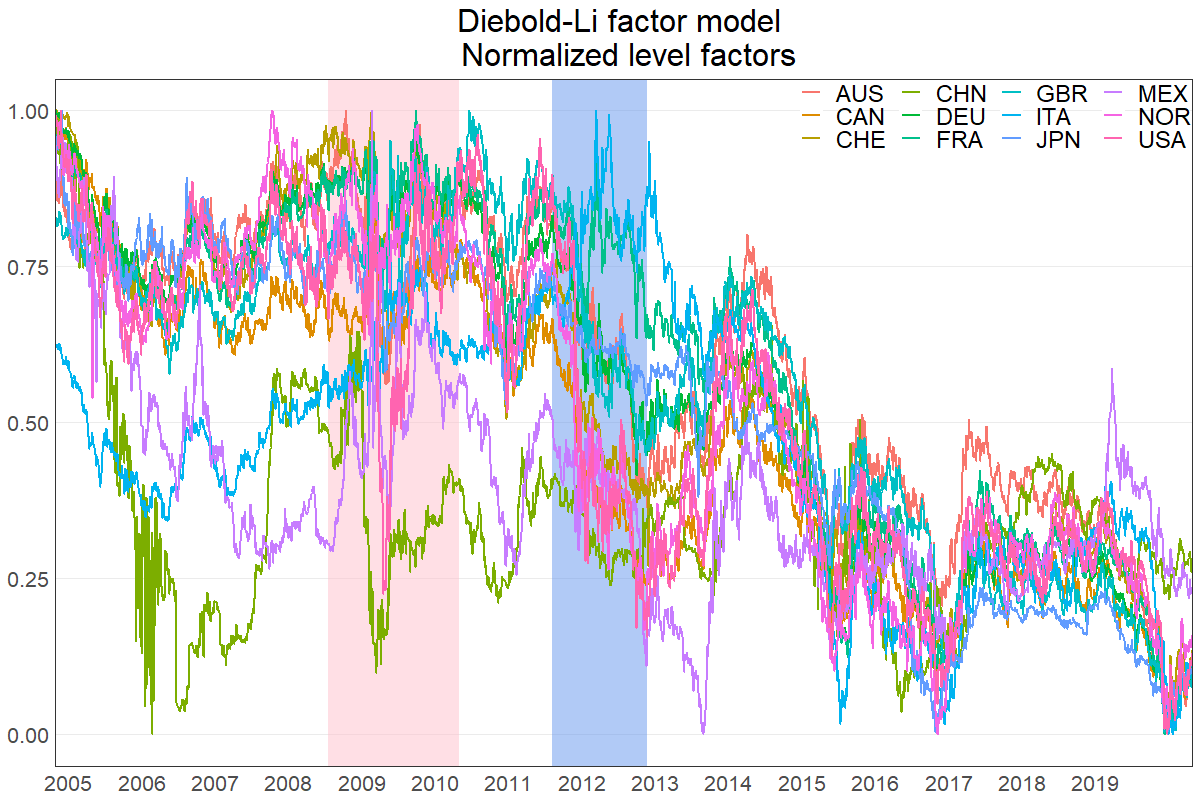
\includegraphics[width=\linewidth]{Normalizedlevel}
\caption{\textbf{Szint}}

\end{subfigure}%
\begin{subfigure}{.5\linewidth}
\centering
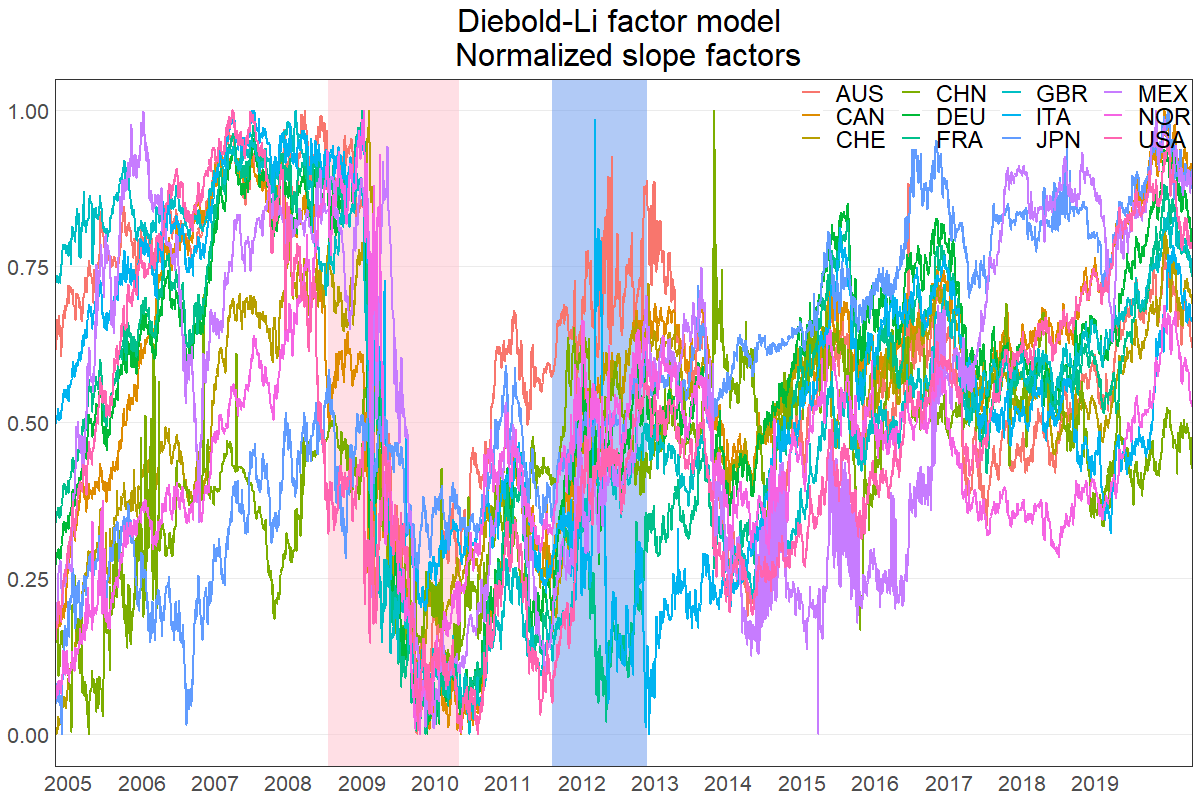
\includegraphics[width=\linewidth]{Normalizedslope}
\caption{\textbf{Meredekség}}
\end{subfigure}\\[1ex]
\begin{subfigure}{.5\linewidth}
\centering
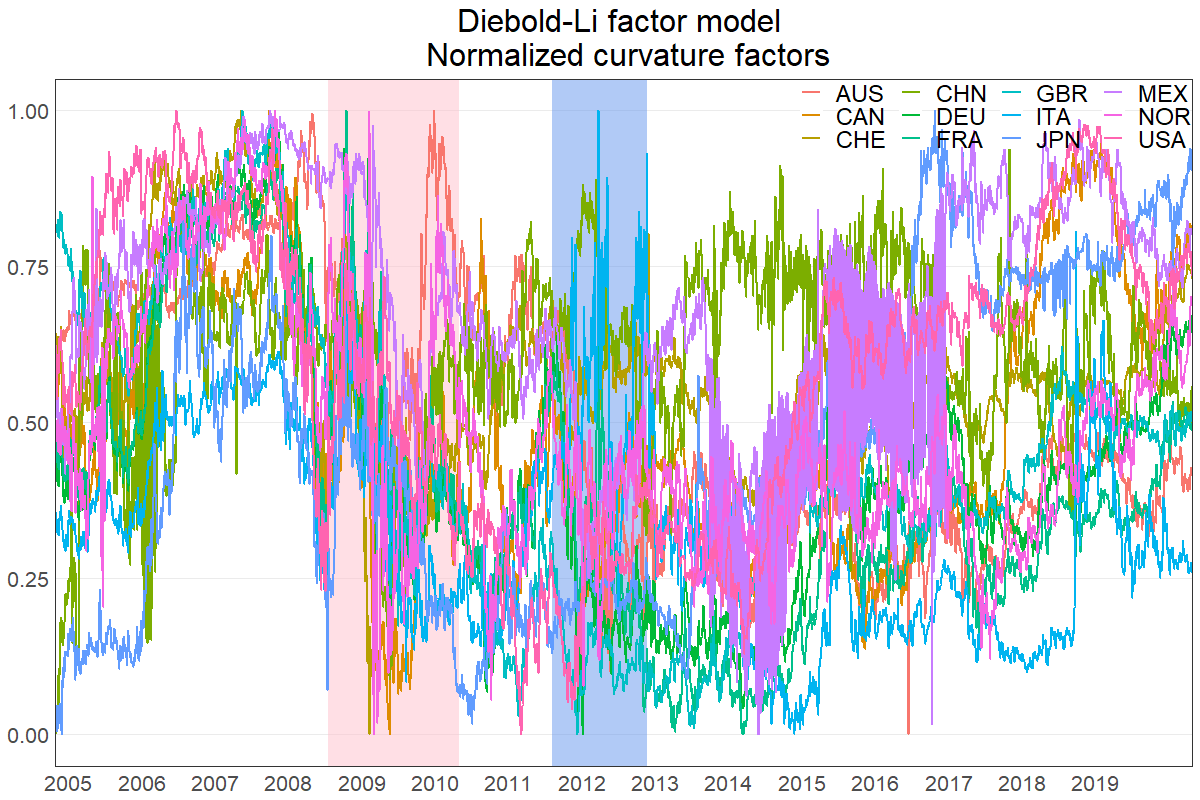
\includegraphics[width=\linewidth]{Normalizedcurvature}
\caption{\textbf{Görbület}}
\end{subfigure}
\end{figure}

%---------------------------------------------------------------------------------------------------------------------------------------------------------------------------

 Leíró statisztikájukat az 1. táblázat tartalmazza. Az átlagos Szint faktor minden ország esetében pozitív, legmagasabb Mexikónál és legalacsonyabb Japánnál. Az átlagos Meredekség a hozamgör-bék tipikus emelkedő alakjára utal (negatív értékek). A Meredekség negatív minden ország esetén, ami azt jelenti, hogy a hosszabb lejáratok magasabban helyezkednek el a rövidebb lejáratoknál. Abszolút értelemben az USA meredeksége a legmagasabb, míg Ausztráliáé a legalacsonyabb. Az esetleges pozitív Meredekségi értékek restriktív monetáris politikai döntésekre utalnak. A görbület is minden alkalommal negatív, legmagasabb Franciaország esetén és legalacsonyab Kínánál (abszolút értelemben).


%-----------------------------------------------------------------------------------Table1-----------------------------------------------------------------------------
\begin{table}[H]
\caption{Hozamgörbe faktorok leíró statisztikája}% title of Table
\fontsize{10}{10}\selectfont
\centering % used for centering table
\begin{tabular}{l c c c c c c}% centered columns (4 columns)
\hline\hline   \\ [-1.5ex]               %inserts double horizontal lines
%Case & Method\#1 & Method\#2 & Method\#3 & test \\  [0.5ex]
Faktor & Átlag & Szórás & Minimum & Maximum & Jarque-Bera t-stat.  & P érték \\ [0.5ex] % inserts table %heading

\hline       \\ [-1.5ex]           % inserts single horizontal line

\textit{Németország}			&		&		&		&		&		&		\\
Szint						&	 2.92 &	1.54	&	-0.34	&	5.41	&	347	&	0.00	\\
Meredekség				&	-1.86	&	1.06	&	-4.54	&	0.14	&	210	&	0.00	\\
\medskip													
Görbület					&	-3.72	&	1.72	&	-7.15	&	0.73	&	234	&	0.00	\\
\textit{Olaszország}			&		&		&		&		&		&		\\
Szint						&	4.78	&	1.29	&	1.98	&	8.00	&	106	&	0.00	\\
Meredekség				&	-3.43	&	1.57	&	-7.01	&	-0.44	&	183	&	0.00	\\
\medskip													
Görbület					&	-4.25	&	2.24	&	-8.60	&	4.75	&	194	&	0.00	\\
\textit{Franciaország}			&		&		&		&		&		&		\\
Szint						&	3.39	&	1.37	&	0.26	&	5.48	&	417	&	0.00	\\
Meredekség				&	-2.24	&	1.19	&	-4.73	&	0.02	&	162	&	0.00	\\
\medskip													
Görbület					&	-4.29	&	1.96	&	-7.82	&	1.07	&	210	&	0.00	\\
\textit{USA}				&		&		&		&		&		&		\\
Szint						&	3.96	&	0.99	&	1.88	&	5.87	&	323	&	0.00	\\
Meredekség				&	-2.41	&	1.55	&	-5.52	&	0.71	&	139	&	0.00	\\
\medskip													
Görbület					&	-3.63	&	2.50	&	-9.58	&	0.72	&	228	&	0.00	\\
\textit{Kanada}				&		&		&		&		&		&		\\
Szint						&	3.43	&	1.10	&	1.23	&	5.90	&	274	&	0.00	\\
Meredekség				&	-1.73	&	1.23	&	-4.84	&	0.58	&	251	&	0.00	\\
\medskip													
Görbület					&	-2.49	&	1.63	&	-6.26	&	1.31	&	206	&	0.00	\\
\textit{Mexikó}				&		&		&		&		&		&		\\
Szint						&	8.58	&	1.28	&	5.56	&	13.41&	834	&	0.00	\\
Meredekség				&	-2.36	&	1.83	&	-6.14	&	0.67	&	340	&	0.00	\\
\medskip													
Görbület					&	-4.16	&	2.85&	-14.84&	0.49	&	321	&	0.00	\\
\textit{Japán}				&		&		&		&		&		&		\\
Szint						&	1.70	&	0.83	&	-0.02	&	3.26	&	406	&	0.00	\\
Meredekség				&	-1.28	&	0.63	&	-2.83	&	-0.02	&	155	&	0.00	\\
\medskip													
Görbület					&	-3.69	&	1.28	&	-6.03	&	-0.87	&	278	&	0.00	\\
\textit{Kína}				&		&		&		&		&		&		\\
Szint						&	4.02	&	0.62	&	2.70	&	6.52 &	2047	&	0.00	\\
Meredekség				&	-1.53	&	0.81	&	-3.87	&	1.65 &	275	&	0.00	\\
\medskip													
Görbület					&	-1.24	&	0.92	&	-5.20	&	1.25&	1128	&	0.00	\\
\textit{Ausztrália}			&		&		&		&		&		&		\\
Szint						&	4.63	&	1.23	&	1.40	&	6.77	&	262	&	0.00	\\
Meredekség				&	-0.89	&	0.98	&	-3.87	&	1.00	&	105	&	0.00	\\
\medskip													
Görbület					&	-2.08	&	1.84	&	-6.59	&	2.25	&	296	&	0.00	\\
\textit{Norvégia}				&		&		&		&		&		&		\\
Szint						&	3.22	&	1.12	&	1.02	&	5.23	&	333	&	0.00	\\
Meredekség				&	-1.22	&	1.07	&	-4.04	&	2.26	&	167	&	0.00	\\
\medskip													
Görbület					&	-1.59	&	1.22	&	-4.68	&	1.73	&	337	&	0.00	\\
\textit{Egyesült Királyság}		&		&		&		&		&		&		\\
Szint						&	3.66	&	1.23	&	0.87	&	5.80	&	329	&	0.00	\\
Meredekség				&	-1.76	&	1.75	&	-5.42	&	1.35	&	211	&	0.00	\\
\medskip													
Görbület					&	-3.33	&	3.02	&	-8.77	&	3.65	&	159	&	0.00	\\
\textit{Svájc}				&		&		&		&		&		&		\\
Szint						&	1.77	&	1.18	&	-0.76	&	3.86	&	289	&	0.00	\\
Meredekség				&	-1.18	&	0.70	&	-3.32	&	0.91	&	219	&	0.00	\\
Görbület					&	-2.94	&	1.21	&	-7.77	&	0.62	&	543	&	0.00	\\

\hline%inserts single line
\end{tabular}
\label{table:nonlin}% is used to refer this table in the text
\end{table}
%----------------------------------------------------------------------------------------------------------------------------------------------------

%------------------------------------------------ table2---------------------------------------------------------------------------------

\bigskip

\begin{table}
\caption{Egységgyök tesztek eredményei}
\fontsize{10}{10}\selectfont
\centering% centering table
\captionsetup{justification=centering}

%------------------------------------------------ ADF table----------------------------------------------------------------------------
\begin{subtable}[t]{1\textwidth}
\centering% centering table
\begin{tabular}{l cc cc cc cc cc cc}
\hline\hline \\ [-1.5ex]                         
 

Ország	&	\multicolumn{2}{c}{DEU}			&	\multicolumn{2}{c}{ITA}			&	\multicolumn{2}{c}{FRA}			&	\multicolumn{2}{c}{USA}			&	\multicolumn{2}{c}{CAN}			&	\multicolumn{2}{c}{MEX}			\\[0.5ex] 

& érték &P 		& érték &P 			& érték &P  		& érték& P         			& érték &P				& érték &P\\

\hline       \\ [-1.5ex] 

Szint	&	-2.30	&	0.45	&	-1.47	&	0.81	&	-2.16	&	0.51	&	-3.66	&	0.03	&	-3.06	&	0.13	&	-3.97	&	0.01	\\
Meredekség	&	-2.09	&	0.54	&	-2.26	&	0.47	&	-1.64	&	0.73	&	-1.50	&	0.79	&	-1.57	&	0.76	&	-1.88	&	0.63	\\
\medskip
Görbület	&	-2.22	&	0.49	&-3.59	&0.03	&	-2.36	&	0.43	&	-1.62	&	0.74	&	-2.35	&	0.43	&	-2.71	&	0.28	\\

\hline   \\ [-1.5ex]    

Ország	&	\multicolumn{2}{c}{JPN}			&	\multicolumn{2}{c}{CHN}			&	\multicolumn{2}{c}{AUS}			&	\multicolumn{2}{c}{NOR}			&	\multicolumn{2}{c}{GBR}			&	\multicolumn{2}{c}{CHE}			\\

 & érték &P & érték &P& érték &P & érték &P& érték &P & érték &P\\

\hline       \\ [-1.5ex] 

Szint	&	-2.97	&	0.17	&	-3.69	&	0.02	&	-2.90	&	0.20	&	-2.63	&	0.31	&	-2.16	&	0.51	&	-2.50	&	0.37	\\
Meredekség	&	-4.85	&	0.01	&	-3.69	&	0.03	&	-2.30	&	0.45	&	-2.72	&	0.27	&	-0.95	&	0.95	&	-3.14	&	0.10	\\
Görbület	&	-2.03	&0.57	&	-5.52	&	0.01	&	-2.61	&	0.32	&	-3.67	&	0.02	&	-1.62	&	0.74	&	-3.14	&	0.10	\\
\hline
\end{tabular}
\caption{\textbf{ADF teszt eredmények}}
\end{subtable}
\hspace{\fill}
%----------------------------------------------------------------------------------------------------------------------------------------------------
\bigskip 

%------------------------------------------------ KPSS table----------------------------------------------------------------------------
\begin{subtable}[t]{1\textwidth}
\centering% centering table
\begin{tabular}{l cc cc cc cc cc cc}% creating eight columns
\hline\hline \\ [-1.5ex]                         %inserting double-line
%Audio Name&\multicolumn{2}{c}{Sum of Extracted Bits}&\multicolumn{4}{c}{Sum of Extracted Bits} \\ [0.5ex] 

Ország	&	\multicolumn{2}{c}{DEU}			&	\multicolumn{2}{c}{ITA}			&	\multicolumn{2}{c}{FRA}			&	\multicolumn{2}{c}{USA}			&	\multicolumn{2}{c}{CAN}			&	\multicolumn{2}{c}{MEX}			\\[0.5ex] 

 & érték &P & érték &P& érték &P & érték &P& érték &P & érték &P\\

\hline       \\ [-1.5ex] 

Szint	&	32.89	&	0.01	&	14.58	&	0.01	&	29.87	&	0.00	&	26.85	&	0.01	&	32.18	&	0.01	&	15.24	&	0.01	\\
Meredekség	&	4.26	&	0.01	&	7.61	&	0.01	&	4.50	&	0.01	&	5.30	&	0.01	&	5.40	&	0.01	&	4.78	&	0.01	\\
\medskip
Görbület	&	8.96	&	0.01	&	10.21	&	0.01	&	15.21	&	0.01	&	7.34	&	0.01	&	4.59	&	0.01	&	4.92	&	0.01	\\


\hline   \\ [-1.5ex]    

Ország	&	\multicolumn{2}{c}{JPN}			&	\multicolumn{2}{c}{CHN}			&	\multicolumn{2}{c}{AUS}			&	\multicolumn{2}{c}{NOR}			&	\multicolumn{2}{c}{GBR}			&	\multicolumn{2}{c}{CHE}			\\

 & érték &P & érték &P& érték &P & érték &P& érték &P & érték &P\\

\hline       \\ [-1.5ex] 

Szint	&	33.94	&	0.01	&	3.55	&	0.01	&	29.17	&	0.01	&	30.06	&	0.01	&	28.70	&	0.01	&	31.96	&	0.01	\\
Meredekség	&	33.21	&	0.01	&	14.99	&	0.01	&	7.32	&	0.01	&	1.25	&	0.01	&	7.53	&	0.01	&	5.49	&	0.01	\\
\medskip
Görbület	&	15.95	&	0.01	&	2.91	&	0.01	&	24.67	&	0.01	&	11.56	&	0.01	&	13.33	&	0.01	&	5.67	&	0.01	\\


\hline
\end{tabular}
\caption{\textbf{KPSS teszt eredmények}}

\end{subtable}
\hspace{\fill}
%----------------------------------------------------------------------------------------------------------------------------------------------------
\bigskip

%------------------------------------------------ ADF(1) table----------------------------------------------------------------------------
\begin{subtable}[t]{1\textwidth}
\centering
\begin{tabular}{l cc cc cc cc cc cc}% creating eight columns
\hline\hline \\ [-1.5ex]                         %inserting double-line
%Audio Name&\multicolumn{2}{c}{Sum of Extracted Bits}&\multicolumn{4}{c}{Sum of Extracted Bits} \\ [0.5ex] 

Ország	&	\multicolumn{2}{c}{DEU}			&	\multicolumn{2}{c}{ITA}			&	\multicolumn{2}{c}{FRA}			&	\multicolumn{2}{c}{USA}			&	\multicolumn{2}{c}{CAN}			&	\multicolumn{2}{c}{MEX}			\\[0.5ex] 

 & érték &P & érték &P& érték &P & érték &P& érték &P & érték &P\\

\hline       \\ [-1.5ex] 

Szint	&	-17.05	&	0.01	&	-16.01	&	0.01	&	-15.99	&	0.01	&	-15.79	&	0.01	&	-16.35	&	0.01	&	-16.56	&	0.01	\\
Meredekség	&	-15.90	&	0.01	&	-14.62	&	0.01	&	-14.59	&	0.01	&	-16.55	&	0.01	&	-16.32	&	0.01	&	-15.19	&	0.01	\\
\medskip
Görbület	&-18.52	&	0.01	&	-18.67	&	0.01	&	-17.65	&	0.01	&	-17.45	&	0.01	&	-16.02	&	0.01	&	-18.88	&	0.01	\\


\hline   \\ [-1.5ex]    

Ország	&	\multicolumn{2}{c}{JPN}			&	\multicolumn{2}{c}{CHN}			&	\multicolumn{2}{c}{AUS}			&	\multicolumn{2}{c}{NOR}			&	\multicolumn{2}{c}{GBR}			&	\multicolumn{2}{c}{CHE}			\\

 & érték &P & érték &P& érték &P & érték &P& érték &P & érték &P\\

\hline       \\ [-1.5ex] 

Szint	&	-16.55	&	0.01	&	-16.99	&	0.01	&	-15.61	&	0.01	&	-16.43	&	0.01	&	-16.48	&	0.01	&	-15.57	&	0.01	\\
Meredekség	&		&		&	-18.90	&	0.01	&	-17.87	&	0.01	&	-17.61	&	0.01	&	-16.12	&	0.01	&	-14.59	&	0.01	\\
\medskip
Görbület	&	-17.51	&	0.01	&		&		&	-18.06	&	0.01	&	-17.04	&	0.01	&	-16.45	&	0.01	&	-14.27	&	0.01	\\



\hline
\end{tabular}
\caption{\textbf{ADF(1) teszt eredmények}}
\end{subtable}
\hspace{\fill}
%----------------------------------------------------------------------------------------------------------------------------------------------------
\bigskip 

%------------------------------------------------ KPS (1) table----------------------------------------------------------------------------
\begin{subtable}[t]{1\textwidth}
\centering
\begin{tabular}{l cc cc cc cc cc cc}% creating eight columns
\hline\hline \\ [-1.5ex]                         %inserting double-line
%Audio Name&\multicolumn{2}{c}{Sum of Extracted Bits}&\multicolumn{4}{c}{Sum of Extracted Bits} \\ [0.5ex] 

Ország	&	\multicolumn{2}{c}{DEU}			&	\multicolumn{2}{c}{ITA}			&	\multicolumn{2}{c}{FRA}			&	\multicolumn{2}{c}{USA}			&	\multicolumn{2}{c}{CAN}			&	\multicolumn{2}{c}{MEX}			\\[0.5ex] 

 & érték &P & érték &P& érték &P & érték &P& érték &P & érték &P\\

\hline       \\ [-1.5ex] 

Szint	&	0.04	&	0.10	&	0.13	&	0.10	&	0.06	&	0.10	&	0.03	&	0.10	&	0.06	&	0.10	&	0.08	&	0.10	\\
Meredekség	&	0.08	&	0.10	&	0.07	&	0.10	&	0.12	&	0.10	&	0.16	&	0.10	&	0.17	&	0.10	&	0.09	&	0.10	\\
Görbület	&	0.05	&	0.10	&	0.02	&	0.10	&0.05	&	0.10	&	0.08	&	0.10	&	0.08	&	0.10	&	0.01	&	0.10	\\


\hline   \\ [-1.5ex]    

Ország	&	\multicolumn{2}{c}{JPN}			&	\multicolumn{2}{c}{CHN}			&	\multicolumn{2}{c}{AUS}			&	\multicolumn{2}{c}{NOR}			&	\multicolumn{2}{c}{GBR}			&	\multicolumn{2}{c}{CHE}			\\

 & érték &P & érték &P& érték &P & érték &P& érték &P & érték &P\\

\hline       \\ [-1.5ex] 

Szint	&	0.03	&	0.10	&	0.16	&	0.10	&	0.05	&	0.10	&	0.04	&	0.10	&	0.07	&	0.10	&	0.04	&	0.10	\\
Meredekség	&	0.03	&	0.10	&	0.03	&	0.10	&	0.04	&	0.10	&	0.08	&	0.10	&	0.24	&	0.10	&	0.14	&	0.10	\\
Görbület	&	0.06	&	0.10	&	0.05	&	0.10	&	0.04	&	0.10	&	0.03	&	0.10	&	0.16	&	0.10	&	0.05	&	0.10	\\


\hline
\end{tabular}
\caption{\textbf{KPSS(1) teszt eredmények}}
\end{subtable}
\hspace{\fill}
%----------------------------------------------------------------------------------------------------------------------------------------------------
%\label{tab:table1}
\end{table}

%----------------------------------------------------------------------------------------------------------------------------------------------------



A faktorok idősorait Jaque-Bera normalitás tesztnek (\cite{bera1981efficient}) vetem alá. Egyik sem teljesíti az elfogadási kritériumot, így az idősorok normalitására vonatkozó nullhipotézist elvetem. Továbbá elvégzem az ADF és KPSS egységgyök teszteket a stacionaritás tesztelésére. Kína Görbület és Japán Meredekség faktora stacionernek bizonyul a szokásos 95\%-os megbízhatósági szint mellett. A többi idősor első rendű differenciázott értékeire elfogadható mindkét előbb említett teszt. 

A differenciázás előtti idősorokat a kointegráció jelenlétének vizsgálata érdekében páronkénti Engle-Granger (\cite{engle1987co}) tesztnek vetem alá. A 3. táblázat a kointegrált és az összes idősorok arányát mutatja faktorok szerint felösszegezve. A főátló mellett a Meredekség-Görbület, illetve a Görbület-Meredekség párok is 70\% feletti értéket mutatnak. Mivel az idősorok nem azonos rendben stacionerek, továbbá magas a kointegrált megfigyelések aránya, indokoltnak tartom a Toda-Yamamoto módszer alkalmazását az összekötöttség vizsgálatához.

%--------------------------------------------------------------------------------Table3 -------------------------------------------------------
\begin{table}[H]
\caption{Blokkosított Engle-Granger teszt} %title of the table

\centering% centering table
\begin{tabular}{l | ccc}% creating eight columns
\hline\hline \\ [-1.5ex]                         %inserting double-line

	&	Szint 	&	Meredekség	&	Görbület	\\
\hline \\ [-1.5ex]  
Szint	&	75.694\%	&	44.444\%	&	64.583\%	\\
Meredekség	&	29.167\%	&	74.306\%	&	71.528\%	\\
Görbület	&	29.167\%	&	78.472\%	&	75.000\%	\\

\hline            
\end{tabular}
\label{table:nonlin}% is used to refer this table in the text
\end{table}

%----------------------------------------------------------------------------------------------------------------------------------------------------


\subsection{Eredmények}

\subsubsection{Statikus összekötöttség}

A Toda-Yamamoto módszerrel kapott összekötöttségi hálózatokat statikus és dinamikus szemlélet szerint is elemzem. A statikus modellbe a rendelkezésre álló összes adatpont bekerült. Az idősorokat maximum egyszer differenciázom, a modellhez szükséges optimális késleltetési szintet pedig az AIC alapján határozom meg. Az 1\%-os szignifikancia szint mellett a modellből nyert oksági kapcsolatokat a 3. ábra mutatja. A Szint faktorokat pirossal, a Meredekséget kékkel, a Görbületet zölddel jelölöm. A két faktor közötti nyíl az okság irányát mutatja, a színe pedig arra a faktorra utal, amelyikből kiindult.

A három alrendszerből a legsűrűbbnek a Meredekségek hálózata bizonyul. A potenciális kapcsolatok 31.06\%-a szignifikáns. Ezt követi a Szint (21.97\%) majd a Görbület (17.42\%). A keresztkapcsolatokat tekintve, az összes Szint faktorból kimenő lehetséges élek 31.25\%-a szignifikáns, a Meredekségeknél ez az arányszám 26.39\%, míg a Görbület ilyen értelemben is a legkevésbé összekötött faktor, a kimenő élek 20.49\%-a szignifikáns.

%--------------------------------------------------------------------------------Fig3 -------------------------------------------------------
\begin{figure}[H]
\caption{Összekötöttség az alhálózatokban}
  \begin{subfigure}[t]{.35\textwidth}
    \centering
    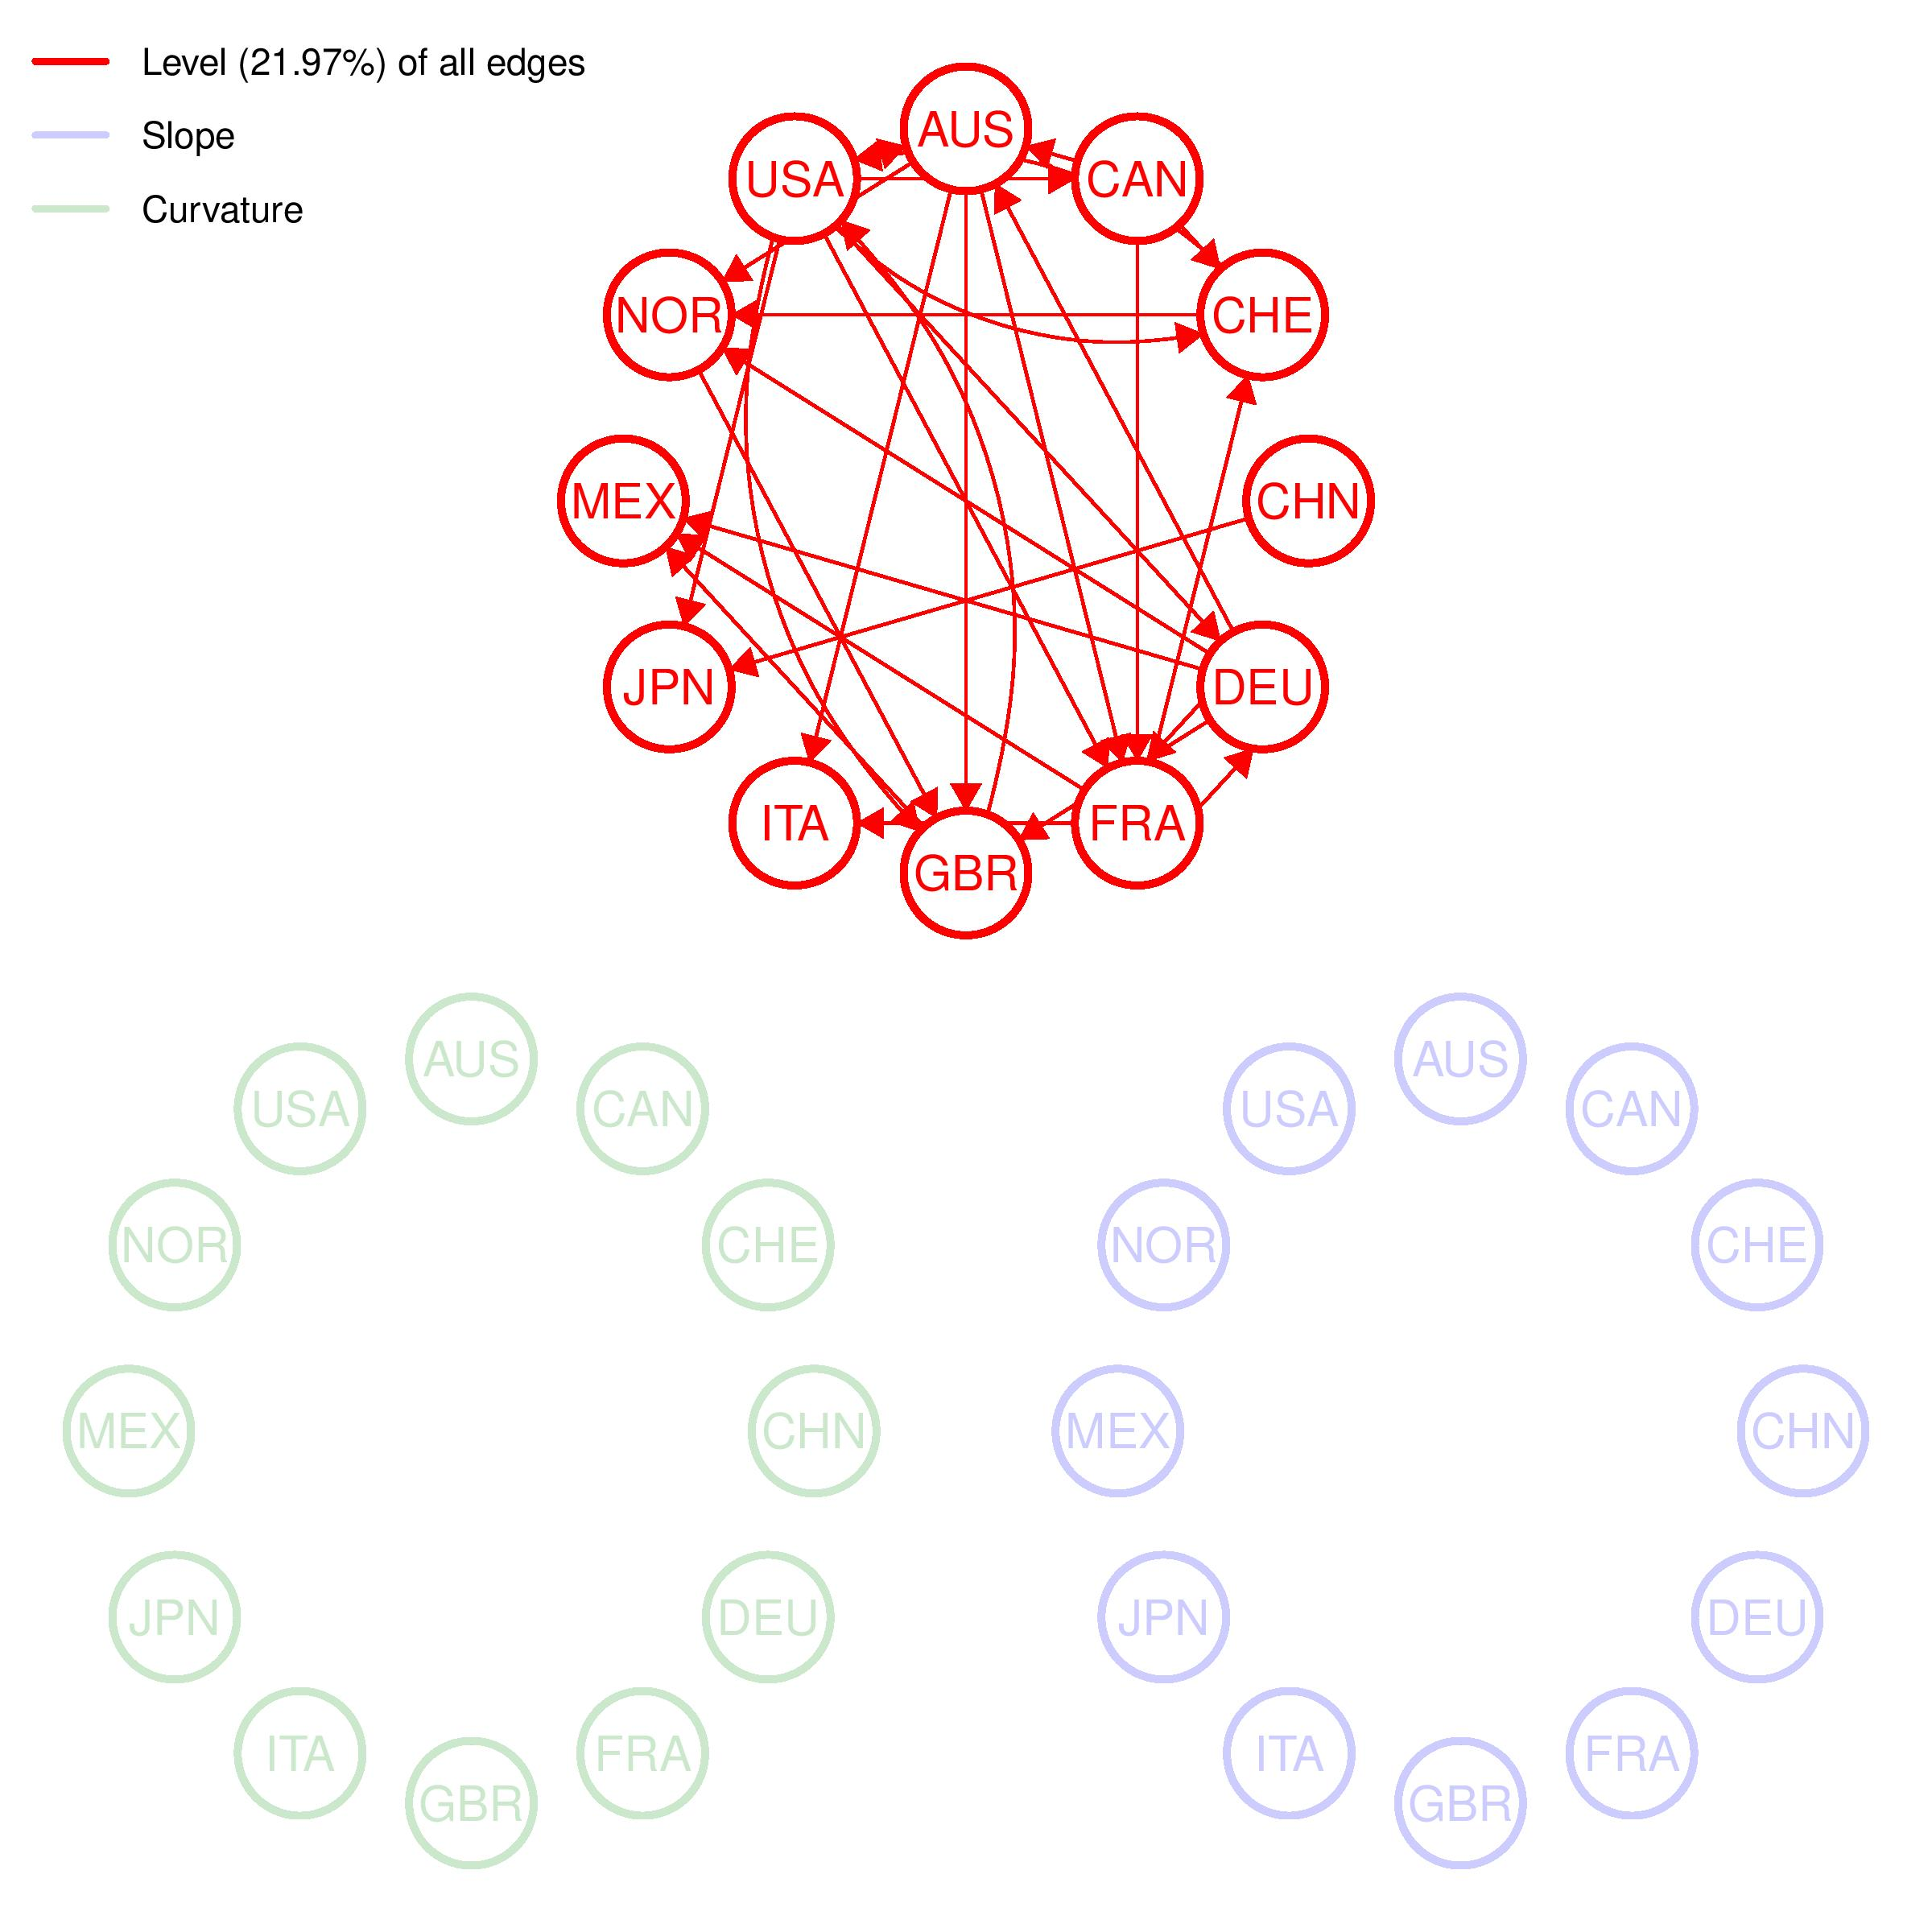
\includegraphics[width=\linewidth]{All_plot_onlylevel2004-07-01_2019-12-31_0.01-page-001}
    \caption{\textbf{Szint alhálózat}}
  \end{subfigure}
  \hfill
  \begin{subfigure}[t]{.35\textwidth}
    \centering
    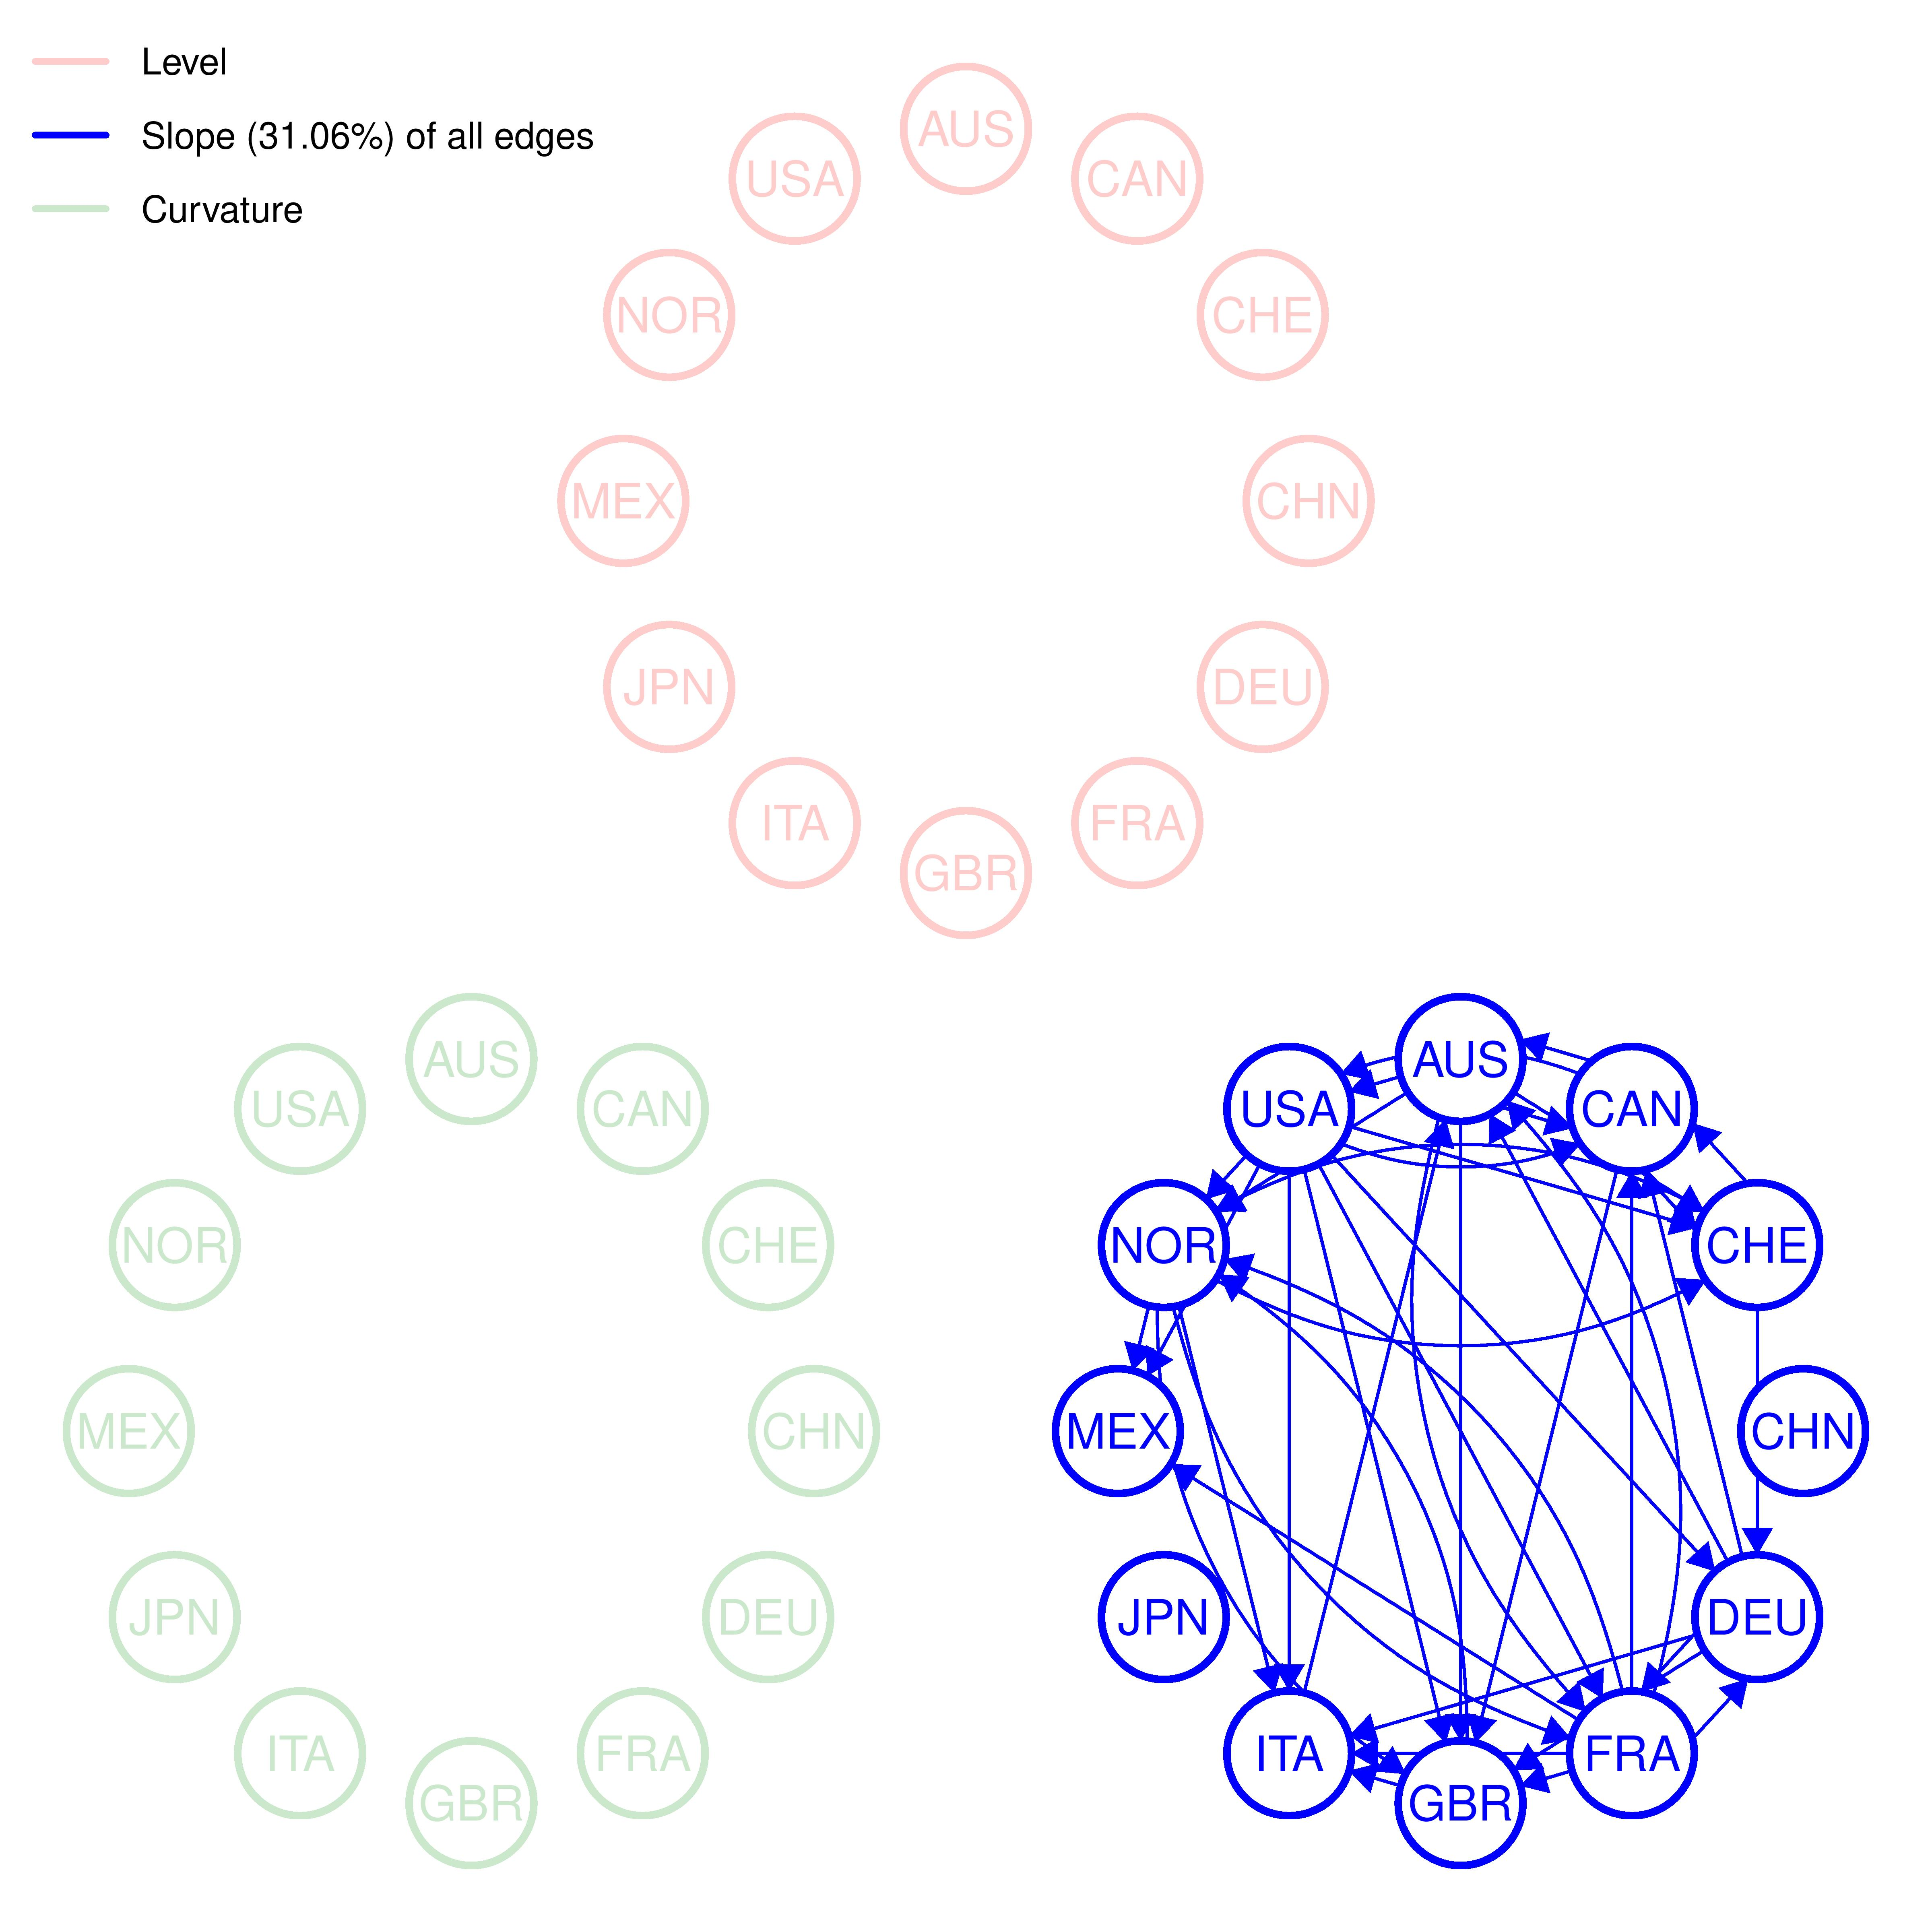
\includegraphics[width=\linewidth]{All_plot_onlyslope_2004-07-01_2019-12-31_0.01-page-001}
    \caption{\textbf{Meredekség alhálózat}}
  \end{subfigure}

  \medskip

  \begin{subfigure}[t]{.35\textwidth}
    \centering
    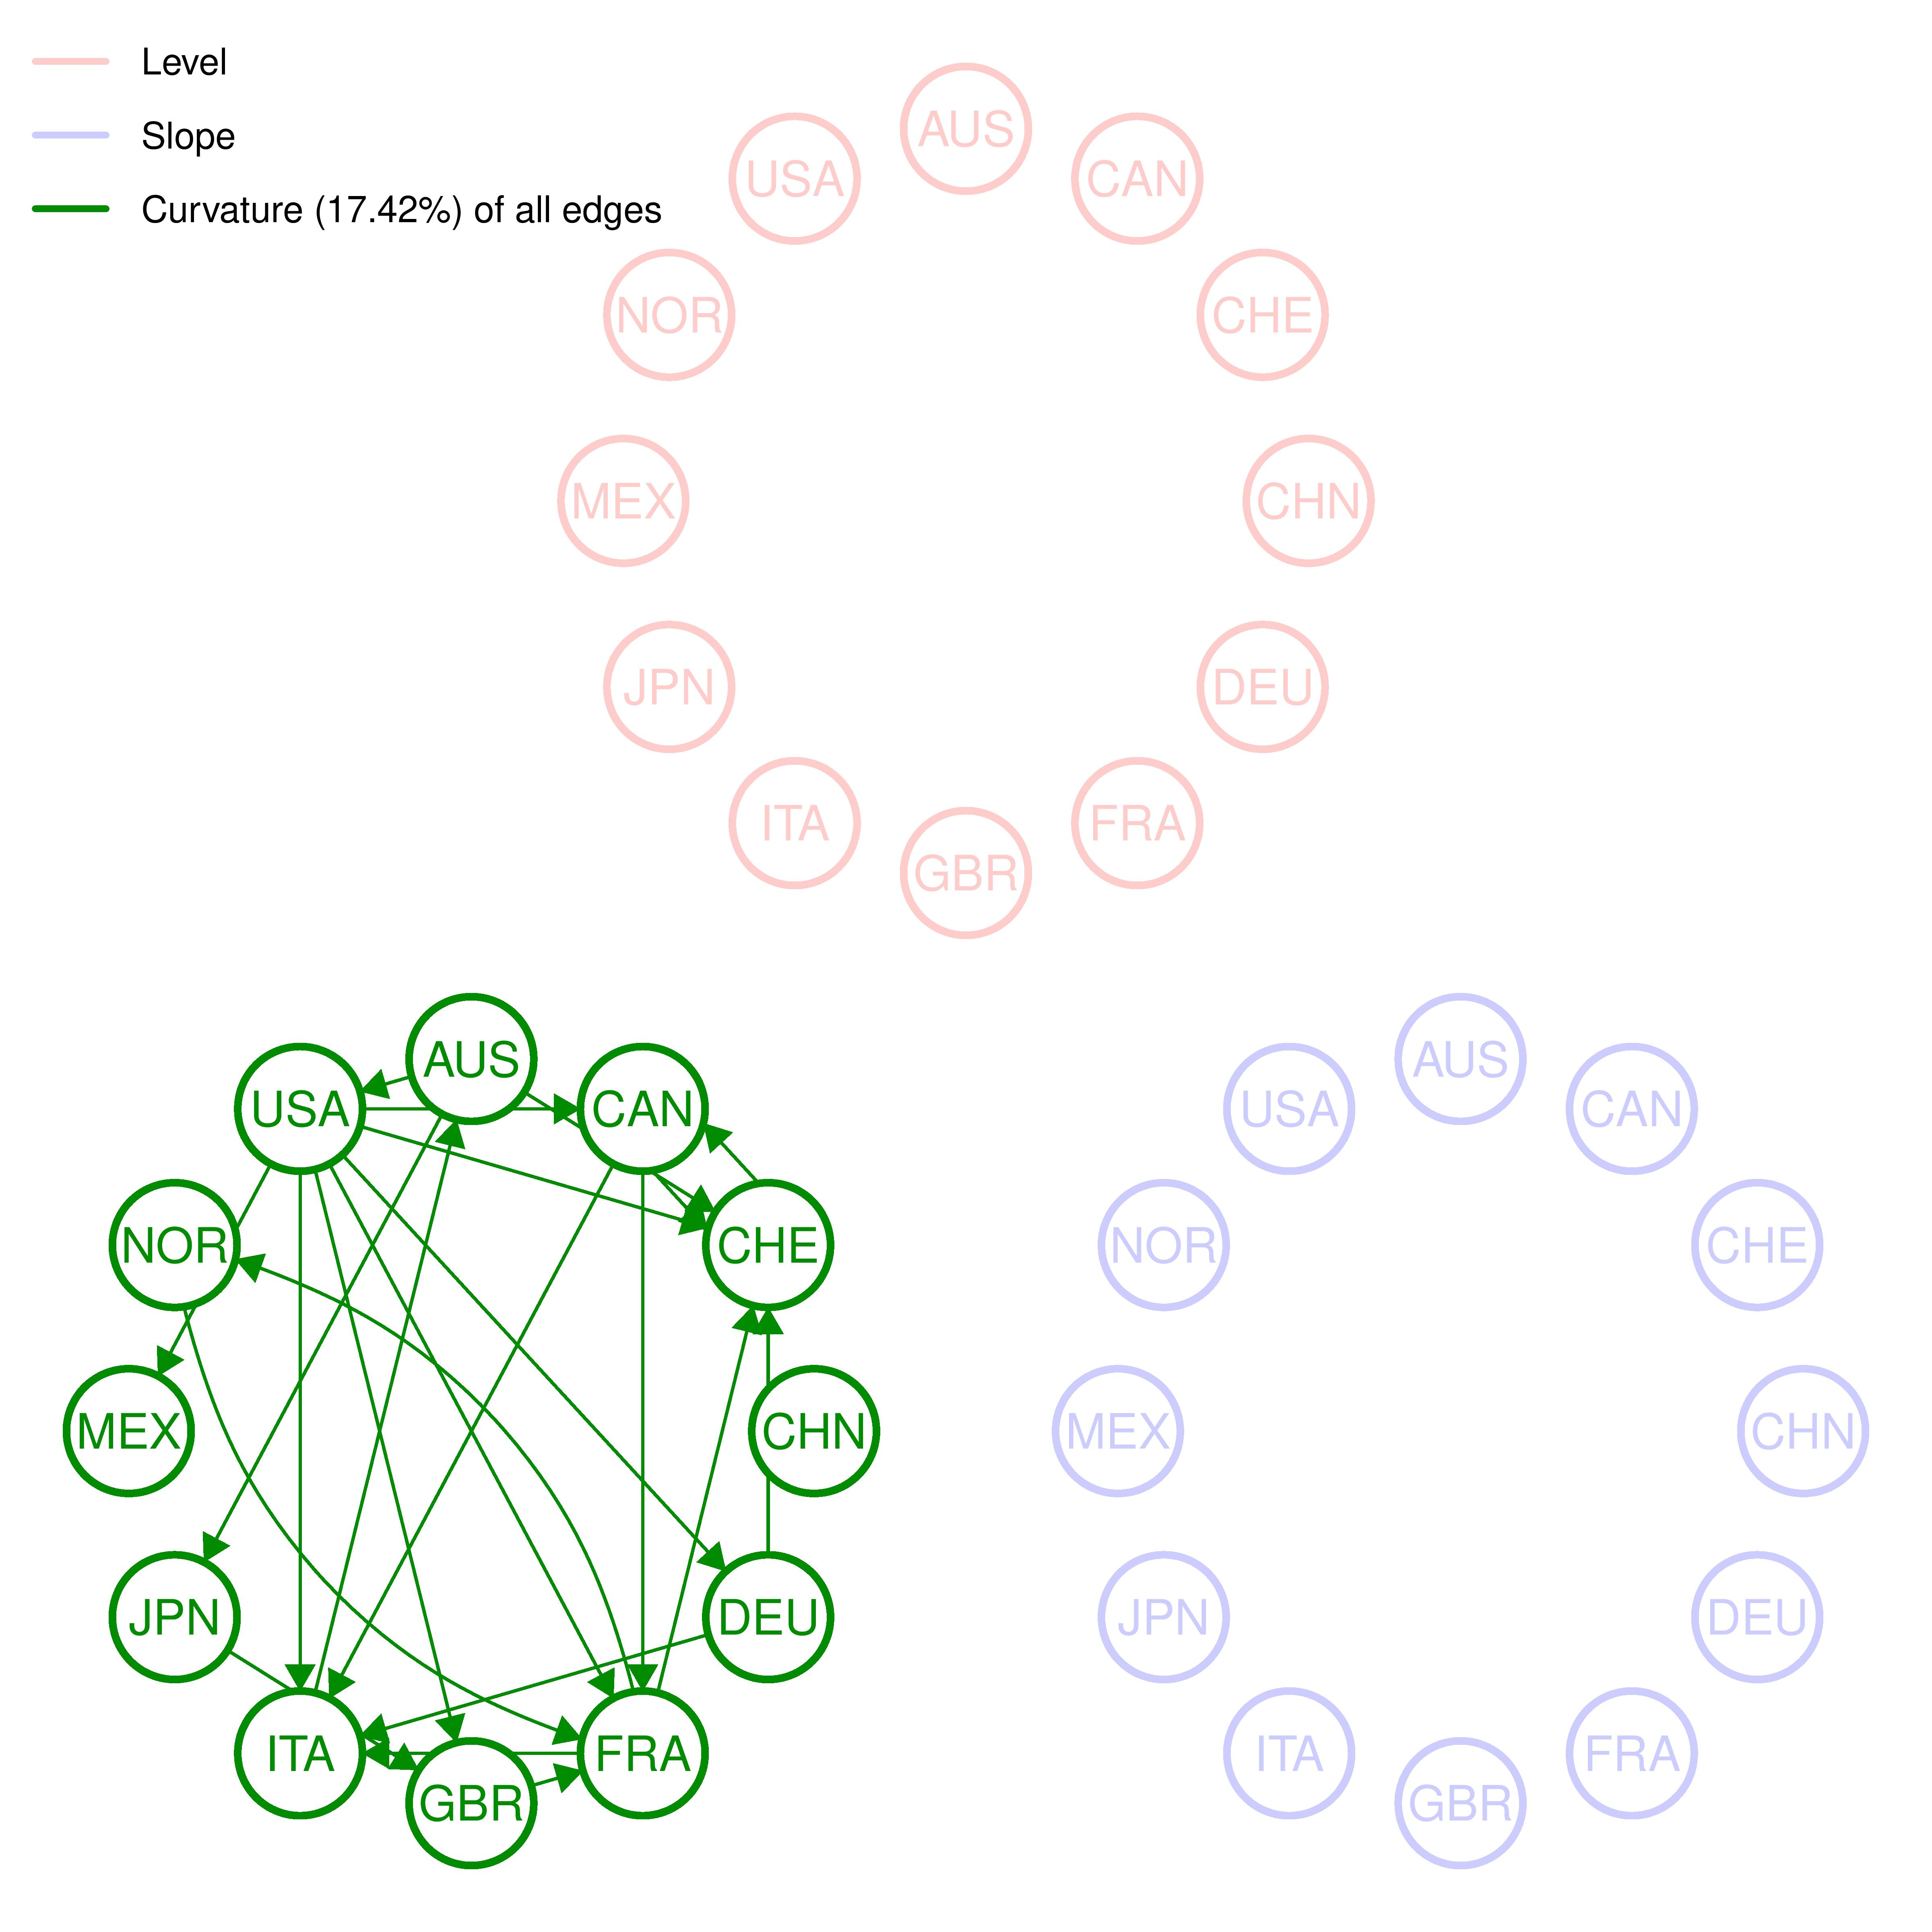
\includegraphics[width=\linewidth]{All_plot_onlycurv_2004-07-01_2019-12-31_0.01-page-001}
    \caption{\textbf{Görbület alhálózat}}
  \end{subfigure}
  \hfill
  \begin{subfigure}[t]{.35\textwidth}
    \centering
    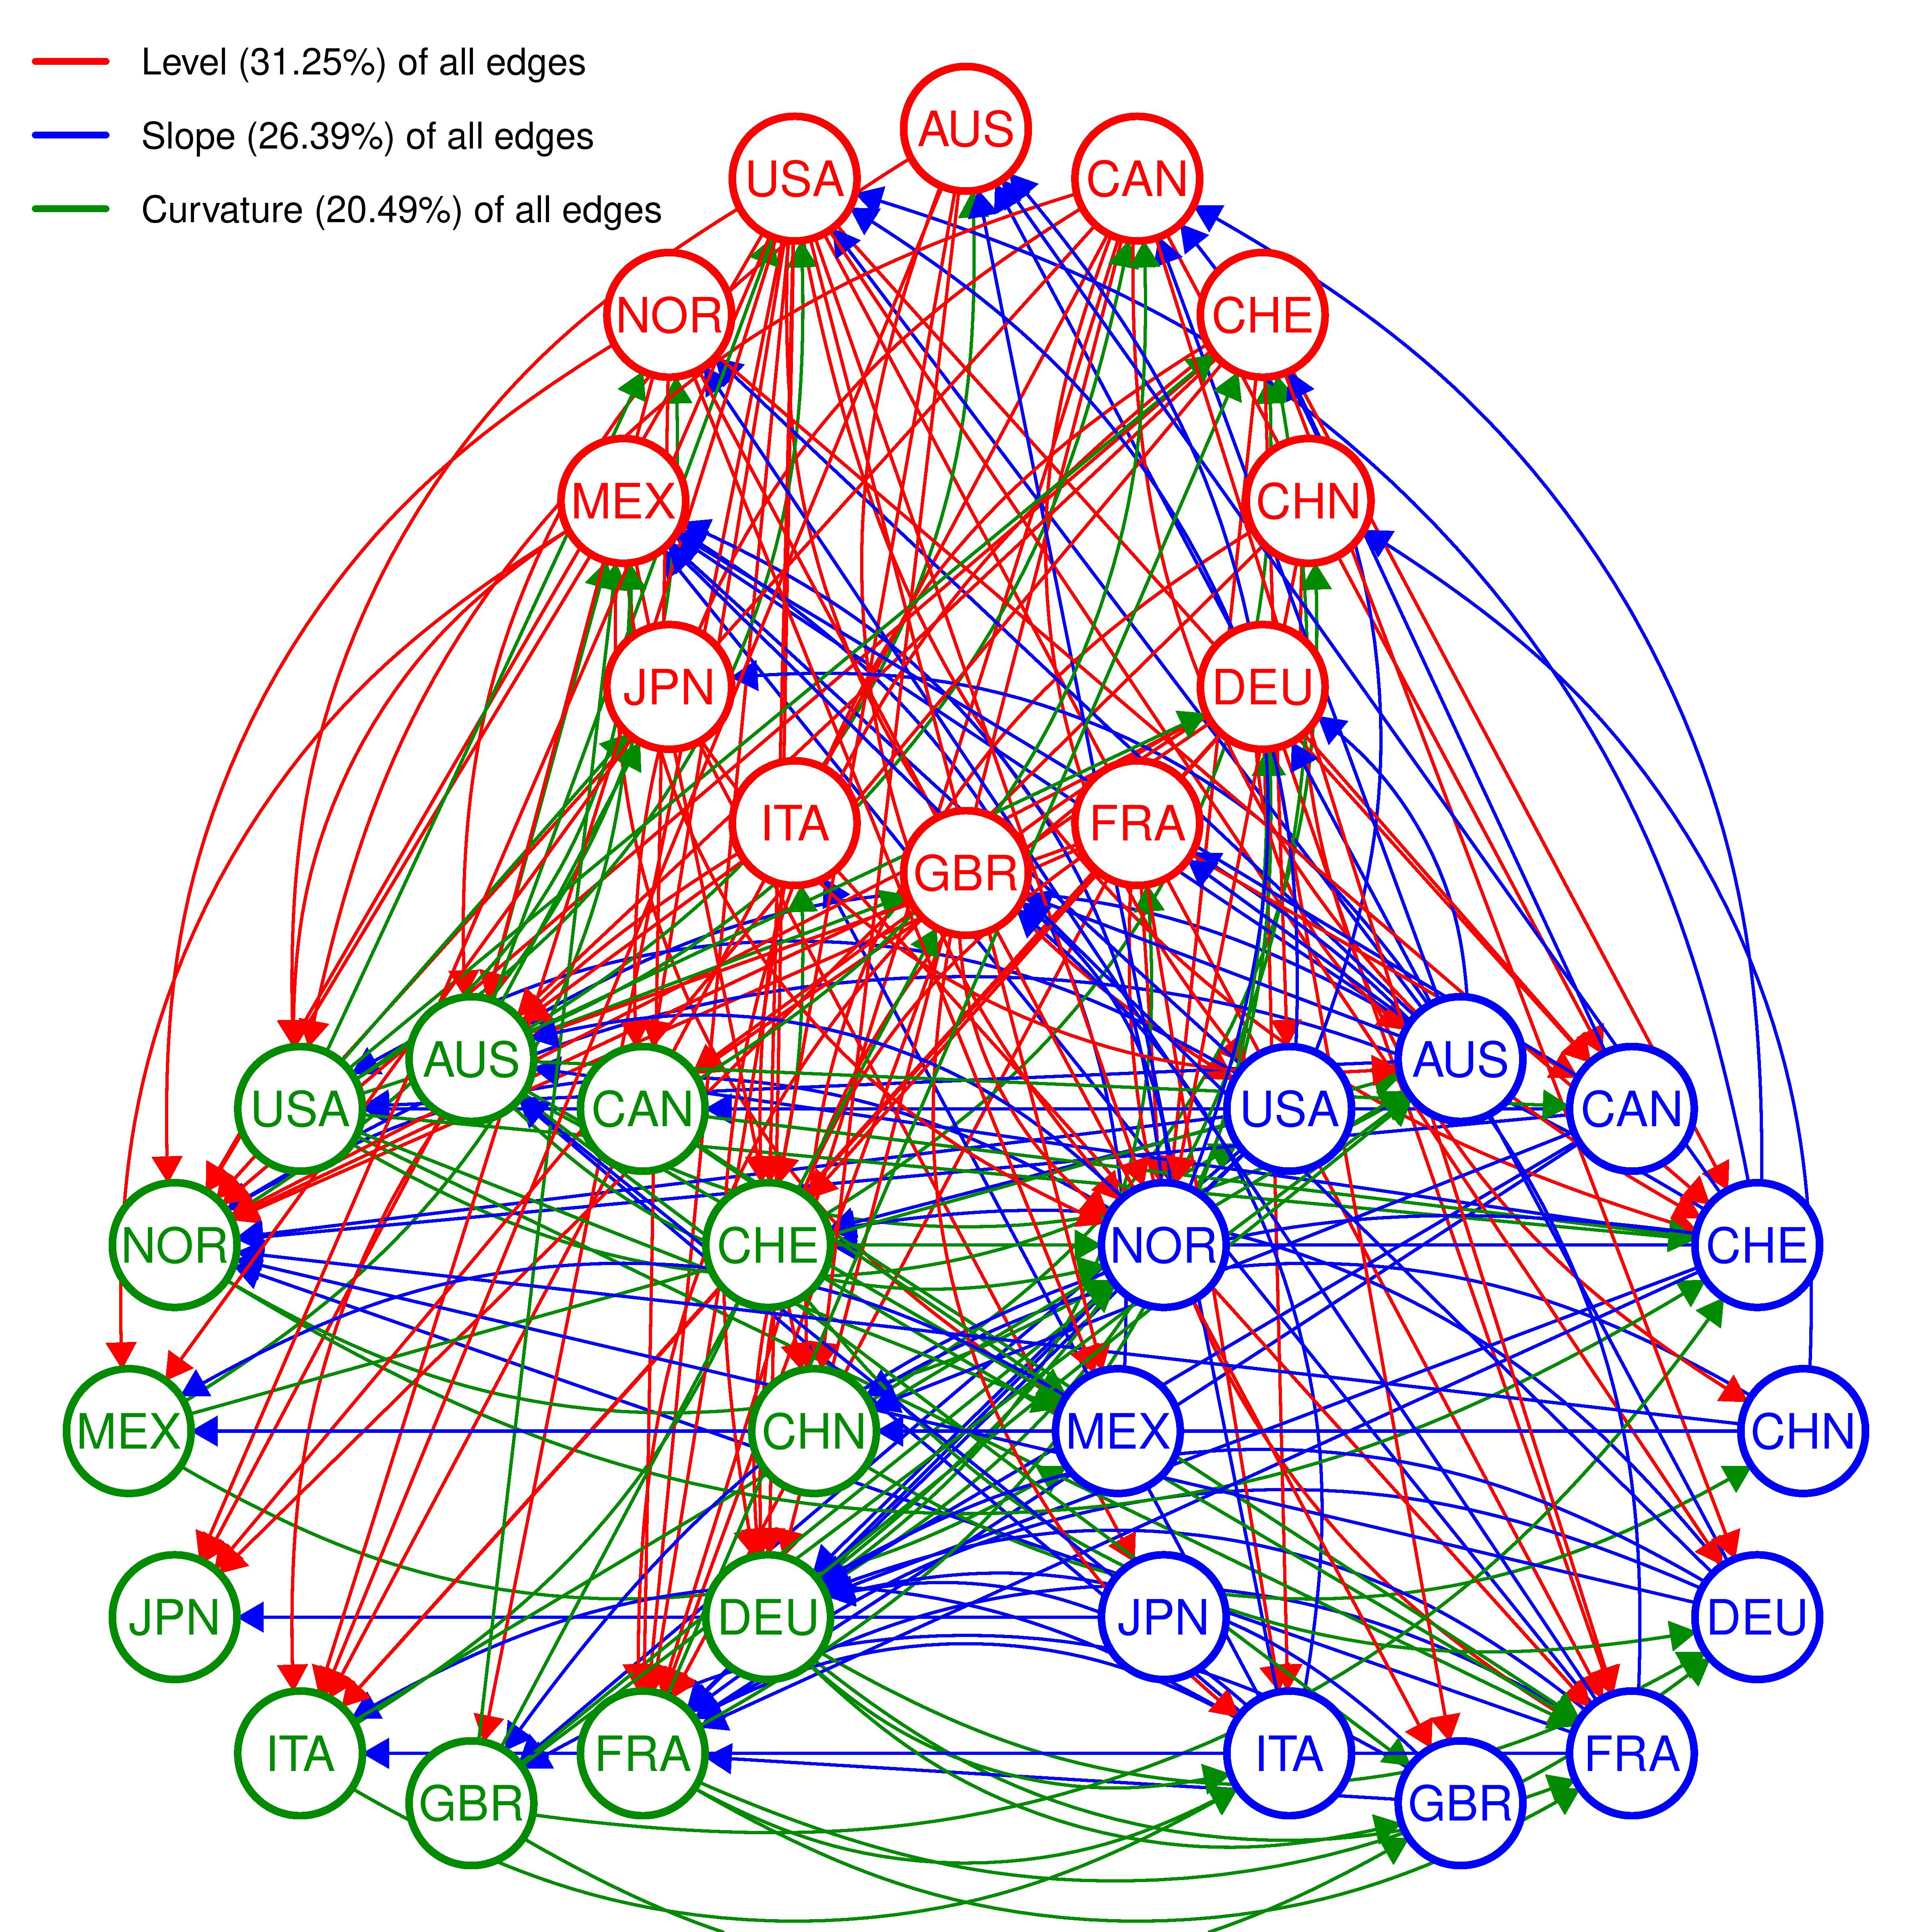
\includegraphics[width=\linewidth]{All_plot_innerempty_2004-07-01_2019-12-31_0.01-page-001}
    \caption{\textbf{Keresztkapcsolatok}}
  \end{subfigure}
\end{figure}

%----------------------------------------------------------------------------------------------------------------------------------------------------

\bigskip

A 4. táblázat (a) része tartalmazza a rendszerben definiált élek számát. A táblázat sorai a kapcsolatok eredetét mutatják, az oszlopok pedig a nyilak végpontjaira utalnak. 1\%-os szignifikancia szinten, a gráfnak 318 éle van, ami az összes lehetséges élnek a 25.24\%-a. A 4. táblázat (b) része tartalmazza az alrendszerek között definiált élek arányát, az abban a viszonyrendszerben értelmezett maximális kapcsolatok számához képest. Ezek alapján elmondható, hogy a Szint és Görbület közötti okság a legsűrűbb, 36.1\%, ezt követi a Meredekség és Görbület közötti összekö-töttség, 31.94\%-kal, a harmadik helyen pedig a Szint alhálózat alatt értelmezett nyilak aránya áll, 31.06\%-kal. A kapcsolati mátrix nem szimmetrikus a főátlóra, a Görbület faktorokból, összesítve kevesebb nyíl irányul mind az alhálózaton belülre, mind kívülre.


%--------------------------------------------------------------------------Table4--------------------------------------------------------------------------


\begin{table}[H]
\caption{A hálózatban definiált szignifikáns élek száma és megoszlása} %title of the table
\fontsize{9}{9}\selectfont
\centering
\begin{subtable}[t]{0.35\textwidth}
\centering
\begin{tabular}{l | ccc  r}% creating eight columns
\hline\hline \\ [-1.5ex]                         %inserting double-line

	&	Szint	&	Meredekség	&	Görbület	& Össz.  \\ 
\hline \\ [-1.5ex]  
Szint	&	29	&	38	&	52	&	119 	\\
Meredekség	&	30	&	41	&	46	&	117	\\
Görbület	&	25	&	34	&	23	&	82	\\
\hline \\ [-1.5ex]  
Össz.	&	84	&	113	&	121	&	318	\\


\hline            
\end{tabular}
\caption{\textbf{Az élek száma, faktorok szerint csoportosítva}}
%\label{table:nonlin}% is used to refer this table in the text
\end{subtable}
\hspace{\fill}
\begin{subtable}[t]{0.5\textwidth}
\centering
\begin{tabular}{l | ccc  r}% creating eight columns
\hline\hline \\ [-1.5ex]                         %inserting double-line



	&	Szint	&	Meredekség	&	Görbület	&	Össz.	\\
\hline \\ [-1.5ex] 
Szint	&	21.97\%	&	26.39\%	&	36.10\%	&	84.47\%	\\
Meredekség	&	20.83\%	&	31.06\%	&	31.94\%	&	83.84\%	\\
Görbület	&17.36\%	&	23.61\%	&	17.42\%	&	58.40\%	\\
\hline \\ [-1.5ex]  
Össz.	&	60.16\%	&	81.06\%	&	85.48\%	&	25.24\%	\\
\hline  
\end{tabular}
\caption{\textbf{Az élek megoszlása, faktorok szerint csoportosítva}}
%\label{table:nonlin}% is used to refer this table in the text
\end{subtable}

\end{table}
%----------------------------------------------------------------------------------------------------------------------------------------------------

A legtöbb éllel rendelkező faktorokat az 5. táblázat szemlélteti. A lista első negyede az összesített kapcsolatokra utal, majd a következő oszlopokban külön fel vannak tüntetve a legtöbb bejövő és kimenő nyíllal rendelkező faktorok. Összességében az Egyesült Államok Szintje rendelkezik a legtöbb éllel, 30-cal. Ugyanakkor ezek közül 23 kimenő él és csak 7 bejövő. Ezt a kapcsolati rendszert mutatja a 4 ábra. Általánosságban elmondható, hogy az USA mindhárom faktora listavezető mind a kimenő, mind a nettó (kimenő - bejövő) élek számának tekintetében is. Ez úgy értelmezhető, hogy az Egyesült Államok mindhárom faktora okozója a többi ország faktorainak, míg ők maguk kevés hatást tapasztalnak a többi résztvevőtől. A kifelé mutató nyilak listájában Ausztrália Görbülete előzi Németország Szint faktorát, míg utóbbi faktor foglalja el a nettó élek listáján a negyedik helyet, Kanada Szintje előtt. A legtöbb oksági hatást kapó faktor a francia Görbület, amit az olasz Meredekség, majd ugyanezen ország Görbülete követ.

%!!!!!!!!!!!!!!!!!!!!!!!!!!!!!!!! CHECK THE TABLE HERE, SOMETHING IS BAD

%--------------------------------------------------------------------------Table5--------------------------------------------------------------------------
\begin{table}[h]
\caption{A legtöbb éllel rendelkező faktorok} %title of the table
\fontsize{10}{10}\selectfont
\setlength{\tabcolsep}{10pt}
\centering% centering table
\begin{tabular}{l  lcc  lc lc  lc}% creating eight columns

\hline\hline \\ [-1.5ex]                         %inserting double-line


\multicolumn{4}{c}{Top 5 Össz.}					&	\multicolumn{2}{c}{Top 5 Bejövő}			&	\multicolumn{2}{c}{Top 5 Kimenő}			&	\multicolumn{2}{c}{Top 5 Nettó}	\\	
\hline \\ [-1.5ex]    
Csomópont	&	Össz. 	&	Be	&	Ki	&	Csomópont	&	Be	&	Csomópont	&	Ki	&	Csomópont	&	Nettó	\\
\hline \\ [-1.5ex]    
USA\_L&	30	&	7	&	23	&	FRA\_C	&	19	&	USA\_L	&	23	&	USA\_L	&	16	\\
AUS\_S	&	28	&	11	&	17	&	ITA\_S	&	16	&	USA\_S	&	18	&	USA\_S	&	12	\\
FRA\_S	&	28	&	14	&	14	&	ITA\_C	&	16	&	USA\_C	&	17	&	USA\_C	&	10	\\
NOR\_S	&	27	&	16	&	11	&	MEX\_L	&	14	&	AUS\_S	&	17	&	DEU\_L	&	9	\\
FRA\_C	&	27	&	19	&	8	&	FRA\_S	&	14	&	DEU\_L	&	16	&	CAN\_L	&	7	\\

\hline            
\end{tabular}
\label{table:nonlin}% is used to refer this table in the text
\end{table}


%----------------------------------------------------------------------------------------------------------------------------------------------------

%--------------------------------------------------------------------------Fig4--------------------------------------------------------------------------
\begin{figure}[H]
\caption{A legtöbb éllel rendelkező csomópont}
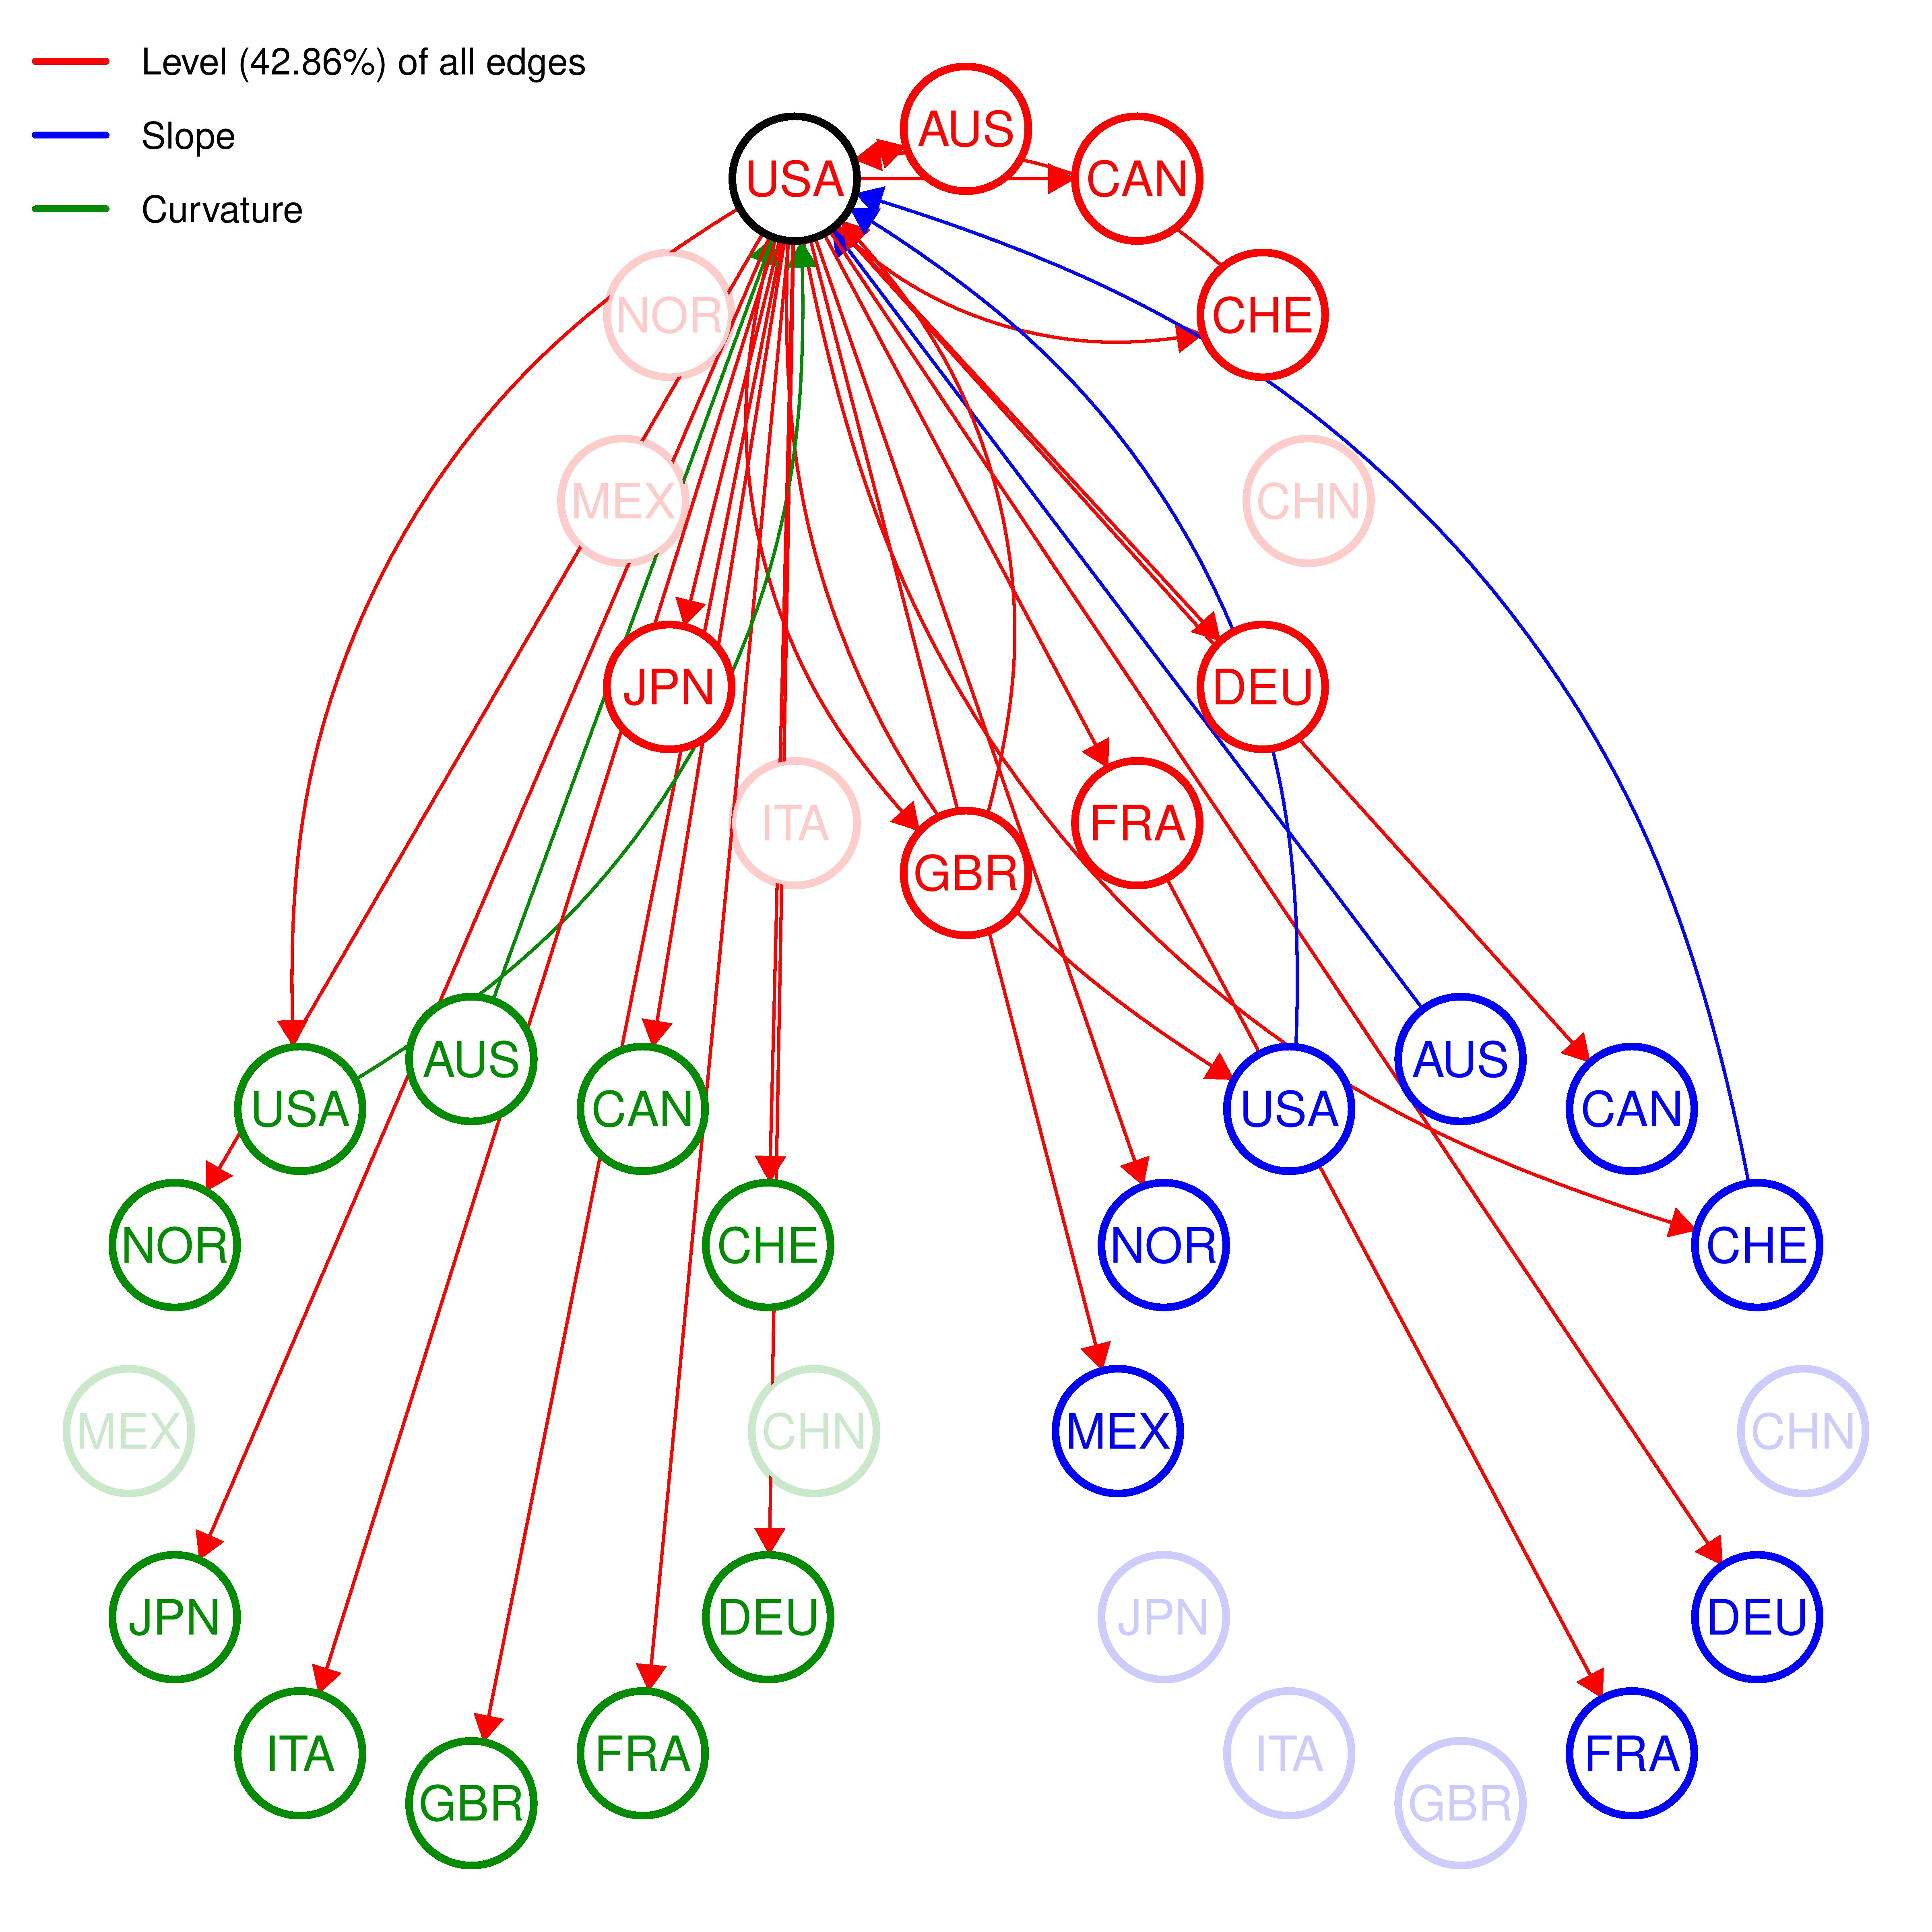
\includegraphics[width=11.5cm]{USA_B_1_plot_2004-07-01_2019-12-31_0.01-page-001}
\centering
\end{figure}

%----------------------------------------------------------------------------------------------------------------------------------------------------

\subsubsection{Idősoros elemzés}

A statikus vizsgálódás után elvégzem az összekötöttségre vonatkozó dinamikus elemzést is. Gördülő időablakom hosszát 750 napnyinak választom meg. Ez 250 munkanapos évet feltételezve 3 évnek feleltethető meg. Minden egyes eltolással 5 napot ugrok, ami munkanapokat feltételezve egy hetet jelent. Így összesen 659 összekötöttséget reprezentáló modellt illesztek. Az ezekből kapott idősorokat mutatja az 5. ábra. A lila vonal a teljes hálózatra vonatkozó szignifikáns élek hányadát jelenti, a türkiz a különböző faktorok alhálózatainak összegét, míg a sárga a keresztkapcsolatok behúzott éleit jelképezi. A piros hátterű időszak a subprime válságra utal, míg a kék hátterű az európai adósságválságra. A periódusokat \cite{bostanci2020connected} alapján választom meg. Ezekben az időszakokban a hálózat összekötöttségi szintje megnövekszik.



%--------------------------------------------------------------------------Fig5--------------------------------------------------------------------------
\begin{figure}[H]
\caption{Dinamikus Toda-Yamamoto elemzés - 750-es ablakméret}
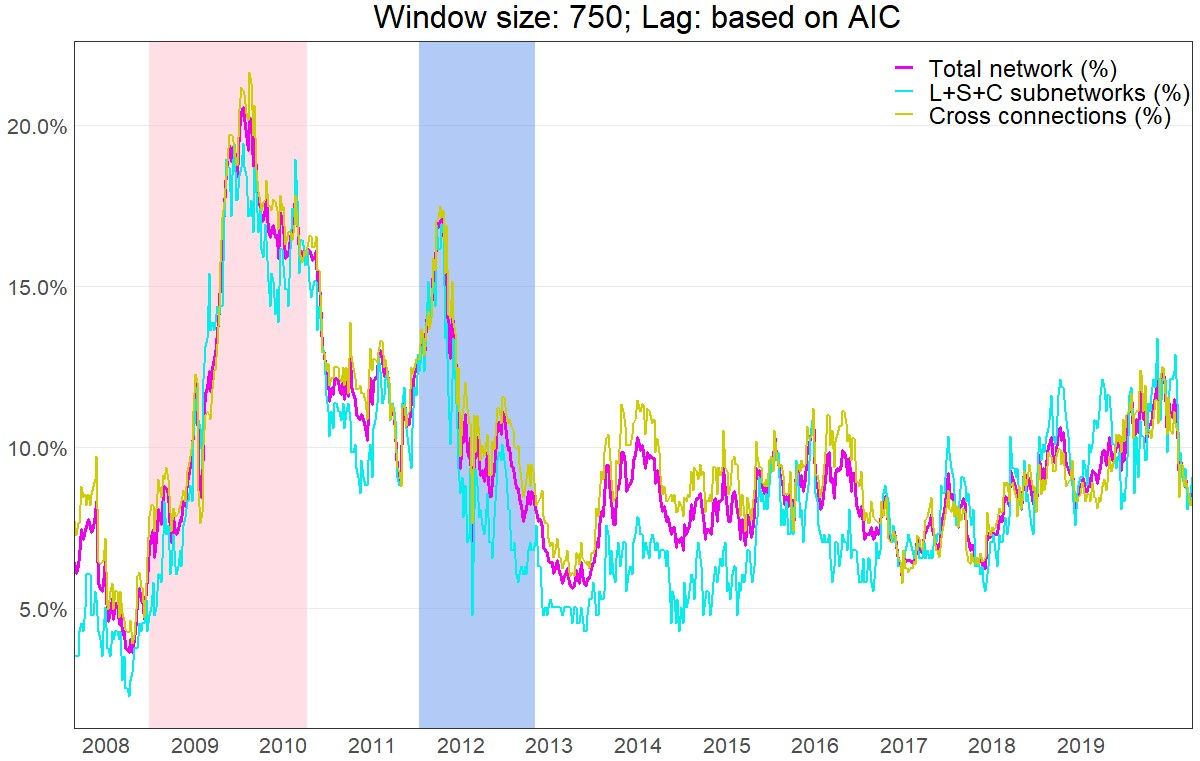
\includegraphics[width=11.5cm]{Time_series_750}
\centering
\end{figure}

A 6. ábra a vizsgált periódus alatt átlagosan letöbb nettósított éllel rendelkező faktorok idősorait mutatja. Ezek növekvő sorrendben: Norvégia Meredekség, USA Görbület és USA Szint. A subprime válság mindhárom faktorra hatással volt, itt az idősorok kiugró értékeket mutatnak. Norvégia Meredekség faktora az európai adósságválság ideje alatt emelkedett meg kimondottan. Ez azzal magyarázható, hogy 2011 végén Norvégia szuverén befektetési alapja eladta a teljes ír és portugál államadósság-állományát, és csökkentette spanyol és olasz kötvényinek tulajdonjogát.
%----------------------------------------------------------------------------------------------------------------------------------------------------

%--------------------------------------------------------------------------Fig6--------------------------------------------------------------------------
\begin{figure}[H]
\caption{A vizsgált periódus alatt legtöbb nettósított éllel rendelkező csomópontok - 750-es ablakméret}
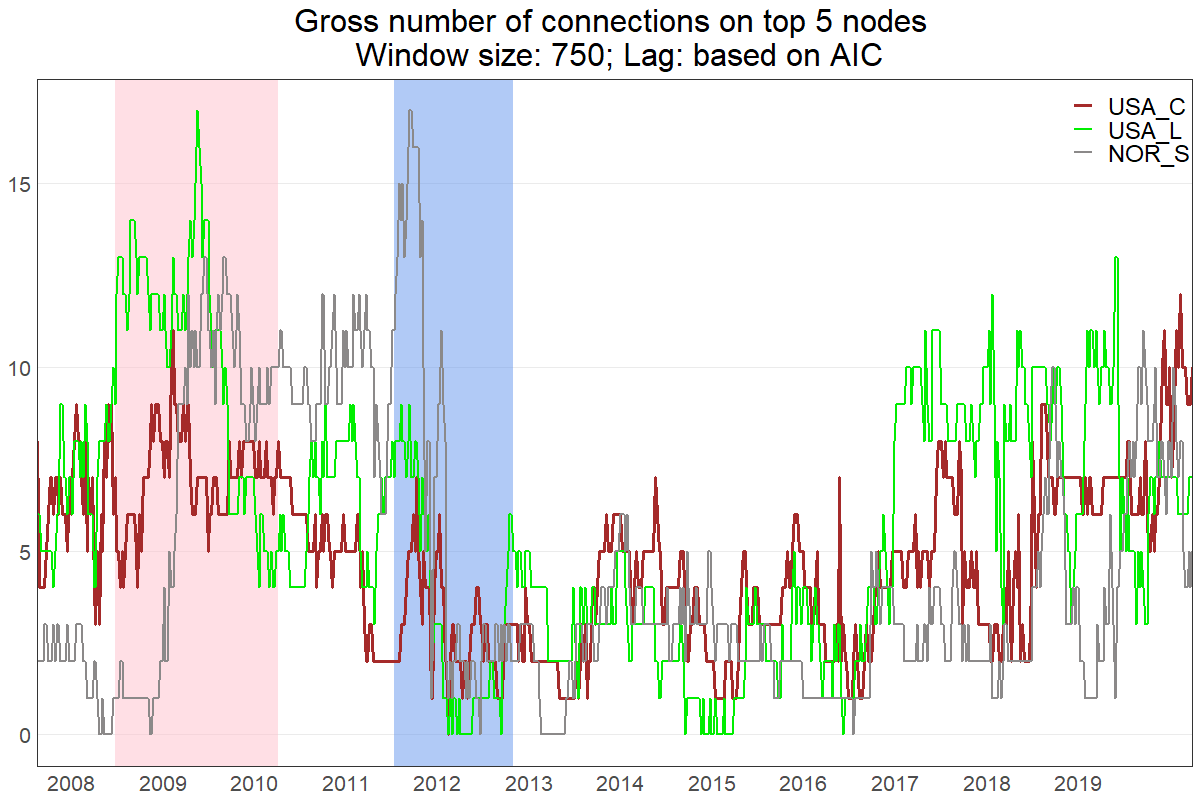
\includegraphics[width=11.5cm]{norway}
\centering
\end{figure}
%----------------------------------------------------------------------------------------------------------------------------------------------------

A 6. táblázat az így kapott öt részidőszak átlagos éleinek számát mutatja be, faktoronkénti bontásban. Jól látható, hogy a subprime válság periódusa alatt minden élszám több, mint duplájára emelkedett. Ezután lassú csökkenés következett, a második válságos periódust a kapott számok nem is tükrözik. Ennek oka, hogy a 2008-as krízis a teljes világra kiterjedt, míg az európai adósságválság alapvetően az európai országokat (főképp az Euro-zónát) érintette. 

%-----------------------------------------------------------------------------------table6------------------------------------------------------------------

\begin{table}[H]
\caption{Az öt részidőszak átlagos éleinek száma - 750-es ablakméret} %title of the table
\fontsize{10}{10}\selectfont
\centering% centering table
\begin{tabular}{l | cccccc}% creating eight columns
\hline\hline \\ [-1.5ex]                         %inserting double-line


		& 	Teljes periódus  &	1. nyugodt	&	1. válság& 	2. nyugodt& 	2. válság&	 3. nyugodt \\
\hline \\ [-1.5ex]  
Szint	&		29	&	7	&	16.2	&	13.4	&  	12.1	&	 12\\
Meredekség	&		41	&	6	&	25.5	&	22.5	& 	16.2	& 	8.6\\
Görbület	&	23	&	7.3	&	20.7	&	9.7	& 	9.2	&	 9.9\\
Keresztkapcsolatok	&		225	&	61.8	&	142.2	&	109.1	& 	101.2	& 	76.1\\
%----------------------------------------------------------------------------------------------------------------------------------------------------

\hline            
\end{tabular}
\label{table:nonlin}% is used to refer this table in the text
\end{table}

Az előbbi dinamikus vizsgálatomat robosztusság tesztnek vetem alá, amit az ablakméret meg-változtatásával érek el. A 7. ábra mutatja a faktorok idősoros alakulását 500-as, illetve 1000-es gördülő ablakméretet választva. Azt tapasztalom, hogy az első esetben a világválság okozta hálózatsűrűsödés itt is látható, de az európai válságra ez a modell érzéketlen. Ez azért lehetséges, mert a Toda-Yamamoto modell érzékeny a bemenő adatsor hosszára (a változók számától függően). Az 1000 megfigyeléses ablakhossz alátámasztja az eredeti esetben kapott eredményeket, mindkét krízisidőszak alatt megfigyelhető a faktorok számának növekedése.

%--------------------------------------------------------------------------Fig7--------------------------------------------------------------------------
\begin{figure}[H]
\centering
\caption{Dinamikus Toda-Yamamoto robosztusság vizsgálat}
\begin{subfigure}{.5\linewidth}
\centering
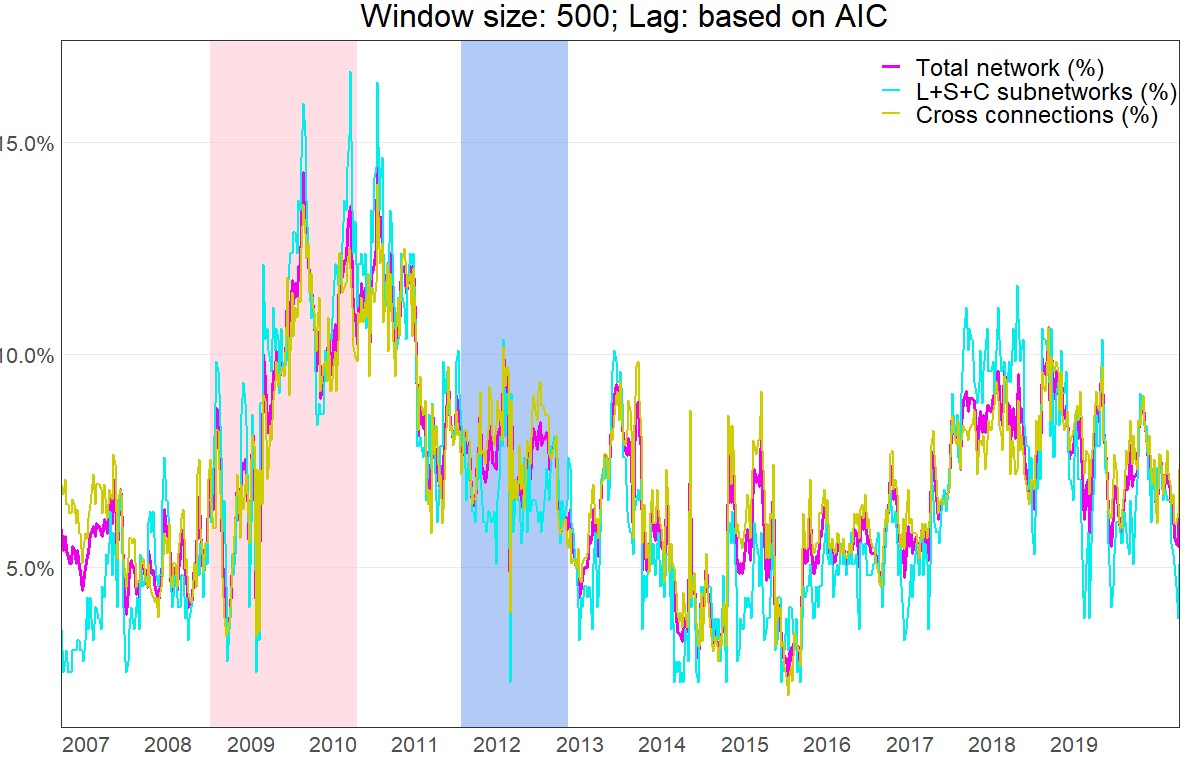
\includegraphics[width=\linewidth]{Time_series_500}
\caption{\textbf{500-as ablakméret}}

\end{subfigure}%
\begin{subfigure}{.5\linewidth}
\centering
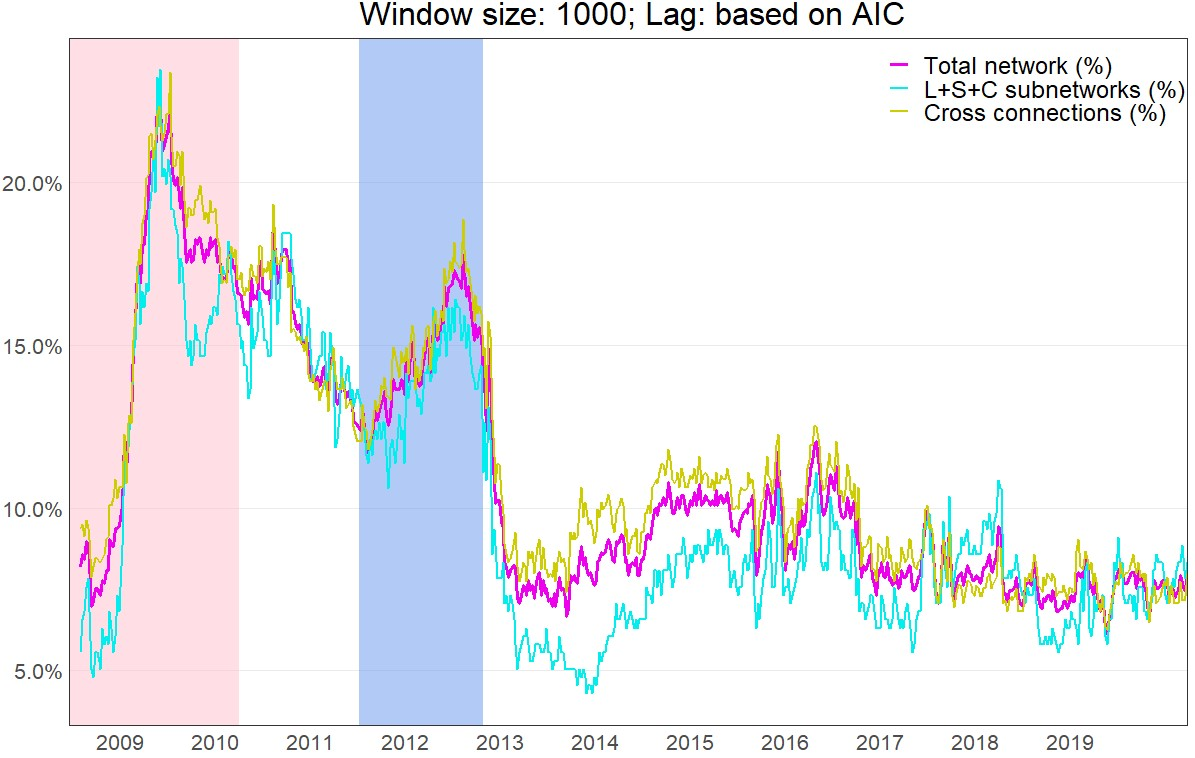
\includegraphics[width=\linewidth]{Time_series_1000}
\caption{\textbf{1000-es ablakméret}}
\end{subfigure}\\[1ex]
\end{figure}
%----------------------------------------------------------------------------------------------------------------------------------------------------

\subsection{Összegzés és további tervek}
Dolgozatomban bemutatom, hogy a 12 szuverénből álló rendszerben az oksági kapcsolatok közül a Szint faktorokból kiinduló élek a legszámosabbak. A Görbület faktorok pedig azok, melyek ezeket leginkább felveszik. Az eddigi tanulmányok nem vizsgálták a faktorok közötti keresztkapcsolatot, pedig kutatásom alapján, nem elhanyagolhatú számú, szignifikáns összekötöttségi él definiálható a rendszerben. A modellezéshez a Toda-Yamamoto eljárást választom, mely hatékonyan kezeli az idősorok között - bizonyítottan fellépő - kointergrációt. Az időablak megváltoztatása mellett szeretném még a hagyományos Granger-i értelemben definiált oksági hálózatot is elkészíteni, melynél sokkal több (hamis korrelációból adódó) élt várok. 

Mindezek mellett szeretném még alkalmazni a \cite{wang2020multilayer} által definiált többrétegű hálózat (mulilayer network) eljárást is. A többrétegű hálózatok élei ugyanazon csomópontok közötti különféle típusú kapcsolatokat reprezentálnak, így alkalmasak az összetett pénzügyi rendszerek integrációjának több dimenziós jellemzésére. Egyelőre kevés cikk foglalkozik a többrétegű hálózatok-kal az információterjesztés szempontjából, így ehhez az irodalomhoz kívánok hozzájárulni.



\newpage 

\section{Összekötöttség részvények volatilitása szintjén}

%Modeling and forecasting volatility lies at the heart of modernfinancebecause good estimates of correlation and volatility are needed forderivative pricing, portfolio optimization, risk management, and hedging

\subsection{Motiváció és irodalmi áttekintés}
Tanulmányomban arra keresem a választ, hogy a volatilitás hogyan terjed egy 20 résztvevőből álló rendszerben. Az elemzési univerzumba 18 olajcég részvényeit választom be, a Föld valamennyi régiójából, piaci kapitalizáció alapján. Ezeket két csoportra osztom elsődleges profiljuk alapján, olajkitermelőkre és olajfinomítókra. Továbbá az elemzés részét képezik még a West Texas Intermediete (WTI) és a New York Harbor Ultra Low Sulfur Diesel (Diesel) leglikvidebb, egy havi határidős termékek is. A Diebold-Yilmaz átterjedési modell alapján azt kapom, hogy a volatilitás elsősorban a kitermelők felől a finomítók felé áramlik, mely hatás a 21 éves vizsgálati periódus alatt felerősödött. A WTI rövid szakaszokra a volatilitás terjesztőjévé tud válni, de ezek valamilyen piaci eseményhez köthető időszakok. Ezen kutatásom még kezdetleges formában van, körülbebül 40\%-os készenléti szinten áll. 

A részvénypiacon az átterjedés (spillover) akkor történik meg, amikor az egyik értékpapír esetén bekövetkező árváltozás késleltetett hatást gyakorol egy (vagy több) másik részvény árára. A szakirodalom megkülönbözteti a hozamok és a volatilitások szintjén értelmezett átterjedést, és az ezek alapján létrehozott összekötöttségi - oksági hálózatokat. \cite{lee1992causal} Granger okságot mér a New York Stock Exchange (NYSE) részvényei között, \cite{hiemstra1994testing} pedig összehasonlítják a lineáris és nem lineáris Granger oksági modelleket, a Dow Jones és a NYSE részvényhozamai esetében. 
Ezen tanulmányomban nem a hozamok átterjedését és ok-okozati kapcsolatait vizsgálom, hanem a volatilisét. A volatilitás megfeleltethető a piacon érzékelhető ''félelemnek'', így azt tudom mérni, hogy az aggodalom hogyan terjed. Másfelől  a különböző instumentumok volatilitása között mért összefüggés azért érdekes, mert szeretném az olajpiac szempontjából válságos periódusokat elemezni és a volatilitás különösen érzékeny a recesszióra. 


A volatilitási hatások átterjedésének mérésére két módszertani csoport terjedt el. Az elsőbe a korreláción alapuló mérőszámok tartoznak, amelyek csak páronkénti összefüggéseket tárnak fel és nagyrészt lineárisak. A korai tanulmányok korrelációhoz kapcsolható módszereket használnak a részvénypiac vizsgálata során (\cite{king1990transmission}, \cite{lee1993does}). Ezt először \cite{bollerslev1990modelling} állandó-, majd \cite{engle2002dynamic} dinamikus feltételes korrelációt alkalmazó modellje haladta meg. A második módszer a Diebold-Yilmaz átterjedési index, melyet, két alfejezettel lejjebb, részletesen is bemutatok.

Az olaj áralakulásával foglalkozó irodalom nagyon gazdag és több évtizedes múltra tekint vissza. A piac működéséről \cite{alhajji2000opec} adnak átfogó képet, amit \cite{balistreri2010oil} tovább árnyalnak és aktualizálnak. 
A nyersolaj más eszközökre gyakorolt hatása szintén népszerű kutatási terület. Az egyik legkézenfekvőbb szempont a második legkereskedettebb energiahordozóval, a gázzal vett összehasonlítás. \cite{batten2017dynamic} azt kapják, hogy a gáz képes volt irányítani az olaj árát, de 2006 után ez a jelenség már nem szignifikáns. \cite{nazlioglu2013volatility} a WTI hatását elemzik az élelmiszer árucikkek volatilitására és azt találják, hogy a globális élelmiszer-válság óta az olaj nettó volatilitás leadó a mezőgazdasági termékek piacára. Az olaj nem csak a commodity piacon képes kifejteni a hatását. \cite{lee2017dynamic} szerint a váratlan pozitív olajár sokkok a nettó kőolaj exportáló országok esetében csökkentik az országkockázatot, nettó importőrök esetén pedig növelik.

Esetemben az olaj árupiaci és részvénypiaci hatásai a legrelevánsabbak. \cite{arouri2012impacts} és \cite{awartani2013dynamic} regionális tőzsdéket vizsgálnak. Míg előbbiek a nyersolaj (WTI és Brent) az európai Dow Jones Stoxx szektor indexek volatilitásaira gyakorolt hatásait vizsgálják, addig a utóbbiak az Öböl Menti Együttműködési Tanács országainak részvényhozam és volatilitás átterjedéseit kutatják a WTI-al szemben. \cite{ma2019spillovers} a WTI hozamok és az amerikai energiaszektor hozamaniak összekötöttségét elemzik és azt kapják, hogy az ipar egésze tudja befolyásolni a WTI árváltozását, de az egyedi részvények lekövetik azt.

A dolgozatom a jelenlegi irodalomhoz képesti hozzájárulása kétrétű. Tudomásom szerint, ezen tanulmány az első, mely az olaijpar egészét az előállítási lánc szempontjából vizsgálja és a volatilitás terjedését ebben a zárt rendszerben modellezi. Továbbá nem találkoztam olyan cikkel, mely a vizsgálati univerzumot kiterjeszti a Föld összes régiójára.


\subsection{Módszertan}
\subsubsection{A volatilitás meghatározása}



A variancia és a volatilitás rokon értelmű szavak, de míg előbbi egy objektív terminológia, addig utóbbi szubjektív. \cite{pagan1996econometrics} megfogalmazásával élve, a volatilitás a bizonytalanság mérőszáma és eszközárak időbeli változását tükrözi, a variancia pedig az adatokból számítható. A volatilitás modellezése a modern pézügyek egyik sarokköve, hiszen olyan területek alapvető hozzávalója, mint a derivatíva árazás, a portfólió optimalizáció és fedezés, vagy a kockázatkezelés. Éppen ezért az irodalom nagyon gazdag ebben a tekintetben. Olyan modellekre van szükség, melyek képesek megragadni az idősorokon megfigyelt stilizált tényeket, például, hogy a hozamok eloszlása lepto-kurtikus (széles végek a normális eloszláshoz képes) és ferde, valamint, hogy a volatilitás klasztereződik (nagy hozam után ismét nagy következik, kicsi hozamot pedig kicsi követ). Ezek alapján három modellcsalád terjedt el:

\begin{itemize}
\item Az \cite{engle1982autoregressive} és \cite{bollerslev1986generalized} nevéhez köthető Generalised Autorgressive Conditional Heteroskedasticity (GARCH) modell és változatai,
\item A sztochasztikus volatilitás (SV) modellek (\cite{hwang2000market}),
\item A különböző volatilitás mértékek, melyek, a napi nyitó (Open), záró (Close), minimum (Low) és maximum (High) árakból számíthatók.
\end{itemize}

Számos kutatás foglalkozott már a GARCH és az SV modellek összehasonlításával (\cite{kat1994volatility}, \cite{andersen1994stochastic}, \cite{kim1998stochastic}, \cite{chan2003using}), de a szerzők különböző eredményekre jutottak. Ezért és a számítás egyszerűsége miatt is döntöttem ezen mérőszám alkalmazása mellett. Ezek közül négyet különböztet meg a szakirodalom. \cite{alizadeh2002range} és \cite{gallant1999using} az alábbi egyszerű módon definiálják a varainciát (a sok szerző miatt itt az idex az S, mint 'simple' jelölést kapta, a többi modellben pedig a szerzők vezetéknevének kezdőbetűivel hivatkozok):

\begin{equation}
V_{S,t}=ln(H_t) - ln(L_t)
\end{equation}

\cite{parkinson1980extreme} egy 0 drifttel rendelkező Geometrikus Brown Mozgást feltételezve az alábbi egyenletet adja a varianciára:

\begin{equation}
V_{P,t}=0.361[ln(H_t/L_t)]^2
\end{equation}

Ezt egészíti ki \cite{garman1980estimation} a nyitó és záró árakkal:

\begin{equation}
V_{GK,t}=0.5[ln(H_t)-ln(L_t)]^2-[2ln(2)-1][ln(C_t)-ln(O_t)]^2
\end{equation}

Amennyiben a modell nem zéró driftű, úgy új mértékre van szükség, melyet \cite{rogers1994estimating} definiálnak:

\begin{equation}
V_{R,t}=[ln(H_t)-ln(O_t)][ln(H_t)-ln(C_t)]+[ln(L_t)-ln(O_t)][ln(L_t-ln(C_t))]
\end{equation}

A fenti egyenletekben az $O$, $C$, $H$, $L$ a $t$ napra vonatkozó nyitó, záró, maximális és minimális árat, míg $V$ a varianciát jelölik. \cite{chan2003using} és \cite{floros2009modelling} összevetik a fent említett mértékeket és azt kapják, hogy a $V_{S,t}$ túlbecsüli a volatilitást, viszont a másik három egyenlet eredménye között nincs jelentős eltérés. Dolgozatomban ezért a Parkinson-féle mérőszámot használom.


\subsubsection{A Diebold-Yilmaz átterjedési index}

\cite{diebold2009measuring} cikkükben bemutatják a volatilitás átterjedési (volatility spillover) mértéküket, melyet a \cite{sims1980macroeconomics} - féle vektor autoregresszív modellek eredményeire épülő becslési hibavariancia dekompozícióra (Forecast Error Variance Decomposition - FEVD) építenek. A variancia dekompozíció azt méri, hogy egy $i$ változó $H$ lépéshosszú előrejelzési hibavarianciája mekkora mértékben tulajdonítható egy másik, $j$ változó innovációjának, ezáltal létrehozva egy intuitív módszert a volatilitás átterjedésének mérésére. Az eljárás ezen formájában két limitációba is ütközik, az egyik az, hogy a VAR módszer Cholesky faktorazonosítást használ, így az eredmény függ a változók sorbarendezésétől. A második pedig az, hogy csak a teljes populációra volatkozó átterjedési index számítható, a szereplőpárok közötti nem. 

\cite{diebold2012better} kiküszöbölik mindkét limitációt a \cite{koop1996impulse} és \cite{pesaran1998generalized} tanulmányaira épülő általánosított VAR modellel, mely nem érzékeny a változók sorrendjére. A módszer megengedi  a korrelált sokkokat, a hibák eloszlásának normalitását feltételezve. Így az egyes változókat érő sokkok nem ortogonálisak.  Ezért az előrejelzési hiba varianciájához való hozzájárulások összege nem szükségszerűen kisebb (vagy egyenlő) mint egy. Egy $P$-ed rendű, $K$ változót tartalmazó VAR-t az alábbi egyenlet jellemez:

\begin{equation}
y_{t}=\sum_{i=1}^{P} \theta_{i} y_{t-i}+\varepsilon_{t} \\
\end{equation}

ahol $y_{t} = y_{1t},...,y_{Kt}$ egy $K$ endogén változóból álló vektor, $\theta_{i}, (i = 1,...P)$  $K\times K$ dimenziójú paraméter mátrixok , $\varepsilon_{t}$ $\sim$ (0, $\sigma$) időben független eloszlású hibavektor, a $(t = 1,...T)$ az időindex, a $(k = 1,...K)$ pedig a változóindex. A (11)-es egyenletet mozgóátlag formában felírva a lenti formula adódik:

\begin{equation}
y_{t}=\sum_{j=0}^{\infty} A_{j} \varepsilon_{t-j} \\
\end{equation}

ahol a $K\times K$ dimenziójú koefficiens mátrixok rekurzív módon $A_{j} = \theta_{1}A_{j-1}+ \theta_{2}A_{j-2}+...+\theta_{p}A_{j-p}$ ahol $A_{0}$ a  $K\times K$ dimenziójú egységmátrix és $A_{j} = 0$ minden $j < 0$ esetén. \cite{diebold2012better} alapján a $H$ lépéshosszú előrejelzési hibavariancia dekompozíció a következő formában írható fel:

\begin{equation}
\phi_{ij}(H)=\frac{\sigma_{jj}^{-1}\sum_{h=0}^{H-1}(e'_{i}A_{h}\Sigma{}e_{j})^{2}} {\sum_{h=0}^{H-1}(e'_{i}A'_{h}\Sigma{}e_{i})} \\
\end{equation}

ahol $\Sigma$ az $\varepsilon$ hibavektor (becsült) varianciamátrixa, $\sigma_{jj}$ a $j$-edik egyenlet hibatagjának szórása, $e_{i}$ pedig egy olyan vektor melynek $i$-edik eleme 1, a többi pedig 0. Ez egy $K\times K$ dimenziójú $\phi{}(H)$ mátrixot eredményez, $\phi{}(H) = [\phi{}_{ij}(H)]_{i,j=1,...,K}$, ahol minden egyes elem a $j$ változó hozzájárulását adja az $i$ változó előrejelzési hibavarianciájához. A főátlóban lévő értékek az $i$ változót érő sokkok saját előrejelzési hibavarianciához való hozzájárulását tükrözik, a főátlón kívüliek pedig a többi $j$ változónak az $i$ változóra gyakorolt (kereszt)hozzájárulását mutatják.

Mivel a saját és kereszthozzájárulások nem adódnak össze eggyé az általánosított VAR alkalmazása miatt, a varianciadekompozíciós mátrix összes elemét normalizálni kell az alábbiak szerint:

\begin{equation}
\bar{\phi}_{ij}(H)=\frac{\phi_{ij}(H)} {\sum_{j=1}^{K}\phi_{ij}(H)} \\
\end{equation}

ahol $\bar{\phi}_{ij}(H)=1$ és $\sum_{j=1}^{K}\bar{\phi}(H)=K$ adódik. Ezáltal meghatározható a teljes átterjedési (Total Spillover) index, százalékos formában:


\begin{equation}
TS(H)=\frac{\sum_{i,j=1,i\neq{}j}^{K}\bar{\phi}_{ij}(H)} {\sum_{i,j=1}^{K}\bar{\phi}_{ij}(H))} \cdot 100= \frac{\sum_{i,j=1,i\neq{}j}^{K}\bar{\phi}_{ij}(H)} {K} \cdot 100 \\
\end{equation}

mely megadja az összes változót érő sokk által okozott átterjedés átlagos hozzájárulását a teljes előrejelzési hibavariaiciához. Ebből levezethető az irányított átterjedés (Directional Spillover). Az $i$ változóba összes többi $j$ változóból érkező átterjedés az alábbiak szerint írható fel: 

\begin{equation}
DS_{i\leftarrow{}j}(H)=\frac{\sum_{j=1,i\neq{}j}^{K}\bar{\phi}_{ij}(H)} {\sum_{i,j=1}^{K}\bar{\phi}_{ij}(H))} \cdot 100= \frac{\sum_{j=1,i\neq{}j}^{K}\bar{\phi}_{ij}(H)} {K} \cdot 100 \\
\end{equation}

míg az $i$ változóból az összes többi $j$ változó felé továbbított átterjedés:
\begin{equation}
DS_{i\rightarrow{}j}(H)=\frac{\sum_{j=1,i\neq{}j}^{K}\bar{\phi}_{ji}(H)} {\sum_{i,j=1}^{K}\bar{\phi}_{ji}(H))} \cdot 100= \frac{\sum_{j=1,i\neq{}j}^{K}\bar{\phi}_{ji}(H)} {K} \cdot 100 \\
\end{equation}

Ha kivonjuk a (14)-es egyenletet a (13)-asból, megkapjuk az $i$ változó nettó átterjedését (Net Spillover) a többi $j$ változó felé:

\begin{equation}
NS_{i}(H)=DS_{i\rightarrow{}j} - DS_{i\leftarrow{}j}
\end{equation}

mely megadja, hogy nettó értelemben véve egy változó továbbítója, vagy pedig felvevője-e a sokkoknak. Végül a nettósított páronkénti átterjedés (Net Pairwise Spillover) felírható a lenti formában:

\begin{equation}
NPS_{ij}(H)=\frac{\bar{\phi}_{ji}(H)-\bar{\phi}_{ij}(H)} {K} \cdot 100
\end{equation}

Az $i$ és $j$ változók közötti páronkénti nettó volatilitási átterjedés egyszerűen az $i$ változóról a $j$-re átgyűrűző bruttó volatilitási sokkok és a $j$ változóról az $i$-re átgyűrűzők különbsége.

\subsection{Adatok}

Tanulmányom adatbázisába 18 részvény került be, valamint a WTI 1 havi határidős árai, emellett pedig a leglikvidebb finomított olajtermék (Diesel) szintén egy havi határidős árai. Az idősorokat a Thomson Reuters adatszolgáltató platformról töltöttem le 2000 januárja és 2020 decembere között. Az adatok napi sűrűségűek, így entitásonként 5283 megfigyeléssel tudtam dolgozni. A vállallatokat két csoportra osztottam a SIC kódjuk alapján: olajfinomítókra (SIC: 2911) és olajkitermelőkre (SIC: 1311). Mindkét csoportba 9-9 vállalat került, a piaci kapitalizációjuk alapján. Olyan cégeket válogattam be, melyek a vizsgált periódus alatt a legnagyobb kapitalizációval rendelkeztek és nem váltottak jogi formát. Nem kerültek be tehát olyan olajipari óriások, mint az Aramco (csak 2019 óta nyilvános részvénytársaság), vagy a Phillips 66 (jelenlegi formájában csak 2012 óta létezik). Az összes feltételnek megfelelő vállalatok tickerjeit, megnevezését, piaci kapitalizációját (millió USD-ben) és elsődleges jegyzésének helyét az alábbi táblázat szemlélteti:

%--------------------------------------------------------------------------table7--------------------------------------------------------------------------
\begin{table}[H]
\caption{Az elemzésbe bevont vállalatok, profil szerint csoportosítva} %title of the table
\fontsize{9}{9}\selectfont
\centering
\begin{subtable}[t]{0.45\textwidth}
\centering
\begin{tabular}{l  lll}% creating eight columns
\hline\hline \\ [-1.5ex]                         %inserting double-line

Ticker	& Vállalat neve	&	Kap.	&	Tőzsde \\ 
\hline \\ [-1.5ex] 
PXD & Pioneer Natural Res Corp		&12543 &	NYSE \\
DVN & Devon Energy Corp					&20551 &	NYSE \\
WPL & Woodside Petroleum Ltd				&19746 &		ASX \\
DVN & Devon Energy Corp					&20551 &	NYSE \\
APA & Apache Corp							&21323 &		NASDAQ \\
CNQ & Canadian Natural Res Ltd		&26719 &		TSX \\
EOG & EOG  Resources Inc					&27799 &		NYSE \\
ONGC & Oil \& Natural Gas Corp Ltd	&32832 &		NSE \\
OXY & Occidental Petroleum Corp			&44351 &		NYSE \\



\hline            
\end{tabular}
\caption{\textbf{Olajkietermelő vállalatok}}
%\label{table:nonlin}% is used to refer this table in the text
\end{subtable}
\hspace{\fill}
\begin{subtable}[t]{0.45\textwidth}
\centering
\begin{tabular}{l lll}% creating eight columns
\hline\hline \\ [-1.5ex]                         %inserting double-line

Ticker	& Vállalat neve	&	Kap.	&	Tőzsde \\ 

\hline \\ [-1.5ex]  
VLO	& Valero Energy Corp	& 20476 & NYSE \\
IMO	& Imperial Oil Ltd	& 26930	& TSX \\
REP	& Repsol YPF	& 27376	& BME \\
SU	& Suncor Energy Inc	& 35852	& TSX \\
RELI& 	Reliance Global Inc	& 52982	& NSE \\
COP	& ConocoPhillips Corp	& 68341	& NYSE \\
BP	& Brittish Petrol Plc	& 157089	& LSE \\
CVX	& Chevron Corp	& 160850	& NYSE \\ 
XOM	& ExxonMobil Corp	& 342248 	& NYSE \\

\hline  
\end{tabular}
\caption{\textbf{Olajfinomító vállalatok}}
%\label{table:nonlin}% is used to refer this table in the text
\end{subtable}

\end{table}

%----------------------------------------------------------------------------------------------------------------------------------------------------

A 18 vállalat több mint fele (10 db) amerikai tőzsdén kereskedett (NASDAQ, NYSE). Három kanadai (TSX), két indiai (NSE), valamint 1-1 spanyol (BME), brit (LSE) és ausztrál (ASX) tőzsdén kereskedett cég került be az elemzési univerzumba. A kapitalizációjukat tekintve az állapít-ható meg, hogy a finomító üzletág négyszerese a kitermelőkének. 

A varianciát a napi záró és nyitó árakból számoltam \cite{parkinson1980extreme} módszere alapján. Mivel a volatilitás a megfigyelések alapján ferde, érdemes log-volatilitásokkal számolni, mely jól közelíti a normális eloszlást. Ahhoz, hogy az évesített százalékos szórást megkapjam (amit a volatilitással azonosítok), az alábbi transzformációt alkalmazom:

\begin{equation}
\sigma_{it}=sinh^{-1}(\sqrt{252\cdot{} V_{P,it}}) \\
\end{equation}

\cite{aihounton2019units} szerint az inverz hiperbolikus szinusz függvény jó helyettesítője a logaritmusnak, a jobbra ferde és 0-t (vagy negatív értékeket) is tartalmazó változók esetén. A felölelt periódus 21 év, így átlagolva 251.6 kereskedési nap jut egy évre, ezért 252 napos évvel számolok. A vizsgált instumentumok számolt volatilitásának grafikonját a 8. ábra mutatja, leíró statisztikájukat pedig a 8. táblázat szemlélteti.

%-----------------------------------------------------------------fig8-----------------------------------------------------------------------------------
\begin{figure}[H]
\caption{A 18 vállalat és a két árupiaci határidős termék volatilitása}
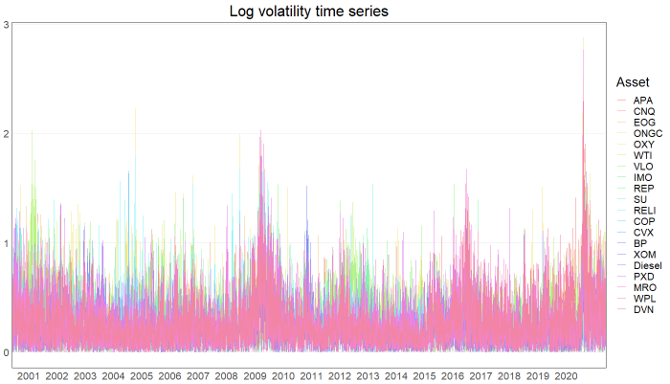
\includegraphics[width=11.5cm]{volatility}
\centering
\end{figure}

\begin{table}[H]
\caption{A 18 vállalat és a két árupiaci határidős termék volatilitásának leíró statisztikája profil szerint csoportosítva} %title of the table
\fontsize{9}{9}\selectfont
\centering
\begin{subtable}[t]{0.45\textwidth}
\centering
\begin{tabular}{l | l l l l l l}% creating eight columns
\hline\hline \\ [-1.5ex]                         %inserting double-line
%----------------------------------------------------------------------------------------------------------------------------------------------------
		
%---------------------------------------------------------------------tabe8-------------------------------------------------------------------------------
Ticker &Átlag	&Medián	&Szórás	&Min&	Max \\
\hline \\ [-1.5ex] 
PXD		&0.31&	0.27&	0.17&	0.06&	1.58 \\
MRO	&0.29&	0.24&	0.17&	0.05&	2.08 \\
WPL		&0.18&	0.15&	0.11&	0.01&	1.38 \\
DVN	      &0.29&	0.25&	0.17&	0.05&	1.61 \\
APA		&0.29&	0.25&	0.18&	0.05&	2.01 \\
CNQ		&0.26&	0.23&	0.15&	0.03&	1.56 \\
EOG		&0.29&	0.25&	0.16&	0.06&	1.60 \\
ONGC	&0.31&	0.26&	0.18&	0.00&	2.08 \\
OXY		&0.25&	0.20&	0.16&	0.03&	2.20 \\
WTI	      &0.27&	0.24&	0.16&	0.01&	2.24 \\



\hline            
\end{tabular}
\caption{\textbf{Olajfinomító vállalatok}}
%\label{table:nonlin}% is used to refer this table in the text
\end{subtable}
\hspace{\fill}
\begin{subtable}[t]{0.45\textwidth}
\centering
\begin{tabular}{l | l l l l l l}% creating eight columns
\hline\hline \\ [-1.5ex]                         %inserting double-line



Ticker &Átlag	&Medián	&Szórás	&Min&	Max \\
\hline \\ [-1.5ex] 
VLO		&0.29	& 0.26	& 0.16	& 0.04	& 1.52      \\
IMO	      &0.22	& 0.19	& 0.13	& 0.04	& 1.62      \\
REP		&0.23	& 0.20	& 0.13	& 0.05	& 1.38      \\
SU		&0.25	& 0.21	& 0.15	& 0.05	& 1.50      \\
RELI		&0.27	& 0.22	& 0.17	& 0.06	& 1.60  \\
COP       &0.22	& 0.19	& 0.14	& 0.04	& 1.66      \\
BP		&0.22	& 0.18	& 0.12	& 0.04	& 1.38      \\
CVX		&0.19	& 0.16	& 0.12	& 0.04	& 1.37      \\
XOM	&0.18	& 0.15	& 0.11	& 0.03	& 1.23      \\
Diesel	&0.24	& 0.21     & 0.13	& 0.00     & 1.46    \\

\hline  
\end{tabular}
\caption{\textbf{Olajkitermelő vállalatok}}
%\label{table:nonlin}% is used to refer this table in the text
\end{subtable}

\end{table}
%----------------------------------------------------------------------------------------------------------------------------------------------------
Az olajkitermelők statisztikái jellemzően magasabb értékeket mutatnak, mint a finomítók ugyanezen mutatói. Az első csoport átlaga, mediánja, szórása és maximum értéke rendre 19.6\%,	19.1\%, 21.5\%, 27.82\% többletet mutat a finomítókhoz képest (beleértve a futures-öket is). Ugyanakkor a kitermelők minimum értéke 9.9\%-kal alacsonyabb. Az átlagos volatilitás alapján a legkisebb kapitalizációjú PXD a legvolatilisebb, míg a legnagyobbal rendelkező XOM a legkevésbé. A maximális volatilitást a WTI érte el 2000 szeptember 22-én (mely valószinűleg az Enron energiavállalat csődje miatt realizálódott).



\subsection{Eredmények}

\subsubsection{Statikus eredmények}



%\begin{table}[H]
%\caption{Daily TY} %title of the table
%\fontsize{7}{7}\selectfont
%\centering% centering table
%\addtolength{\tabcolsep}{-3pt} 
%\begin{tabular}{l | cccccccccccccccccccc | c}% creating eight columns
%\hline\hline \\ [-1.5ex]                         %inserting double-line


%		& PXD	&MRO	&WPL	&DVN	&APA	&CNQ	&EOG	&ONGC	&OXY	&WTI	&VLO	&IMO	&REP	&SU		&RELI	&COP	&BP		&CVX	&XOM	&Diesel	&From     \\
%\hline \\ [-1.5ex] 
%PXD		& 80,7	&0,07	&4,79	&0,02	&0,32	&0,78	&0,2		&0,11	&0,57	&0,68	&0,73	&0,5	&1,05	&0,25	&0,55	&1,13	&4,88	&0,94	&0,77	&0,96	&19,3     \\
%MRO	& 1,81	&75,34	&4,33	&2,32	&1,12	&0,16	&2,54	&0,07	&0,69	&0,2		&0,12	&1,56	&1,8		&0,84	&0,31	&0,58	&0,69	&0,45	&4,21	&0,87	&24,66    \\
%WPL		& 0,7	&1,2		&92,33	&0,06	&0,43	&0,09	&0,18	&0,16	&0,15	&0,14	&0,41	&0,32	&0,44	&0,17	&0,35	&0,52	&0,53	&0,35	&0,8	&0,66	&7,67     \\
%DVN		& 1,21	&2,95	&3,76	&78,43	&1,83	&0,52	&0,92	&0,09	&0,32	&0,26	&0,12	&2,08	&0,98	&0,39	&0,18	&0,43	&1,76	&1,64	&0,94	&1,19	&21,57    \\
%APA		& 0,52	&1,75	&2,7		&2,48	&78,51	&0,69	&1,39	&0,11	&0,76	&0,19	&0,24	&3,1		&0,47	&0,31	&0,09	&0,05	&4,31	&1,18	&0,73	&0,4	&21,49    \\
%CNQ		& 0,1	&0,47	&5,29	&0,46	&1,22	&83,23	&0,15	&0,05	&0,23	&0,34	&0,76	&3,36	&0,33	&0,81	&0,44	&0,13	&0,48	&0,31	&1,55	&0,29	&16,77    \\
%EOG		& 0,63	&0,14	&4,04	&0,36	&0,93	&1,32	&82,52	&0,06	&0,23	&0,61	&0,38	&2,37	&0,68	&0,08	&0,29	&0,25	&2,88	&1,05	&0,83	&0,36	&17,48    \\
%ONGC	& 0,62	&0,07	&3,39	&0,13	&1,53	&1,15	&0,95	&79,53	&0,23	&1,63	&0,36	&0,82	&0,2	&0,3	&2,31	&0,38	&0,3	&2,48	&2,57	&1,04	&20,47    \\
%OXY		& 0,29	&0,09	&2,24	&0,08	&1,2		&1,02	&1,48	&1,1		&85,3	&0,05	&0,57	&1,56	&0,29	&0,77	&0,19	&0,06	&2,78	&0,69	&0,18	&0,07	&14,7     \\
%WTI		& 0,37	&0,01	&0,16	&0,03	&0,35	&0,84	&0,36	&0,47	&3,93	&88,04	&0,81	&0,04	&0,83	&0,59	&0,45	&0,14	&0,06	&0,44	&0,87	&1,2	&11,96    \\
%VLO		& 0,27	&0,02	&5,63	&0,11	&1,57	&0,83	&0,76	&0,84	&1,27	&1,39	&81,58	&0,55	&0,86	&1,07	&0,28	&0,53	&1,46	&0,16	&0,56	&0,22	&18,42    \\
%IMO		& 0,43	&0,23	&2,81	&0,04	&0,3		&0,37	&0,44	&0,51	&1,92	&0,74	&0,99	&88,91	&0,22	&0,55	&0,36	&0,25	&0,74	&0,09	&0,04	&0,06	&11,09    \\
%REP		& 0,52	&0,71	&2		&0,26	&0,26	&1,67	&0,62	&0,37	&0,77	&0,86	&0,62	&1,28	&86,12	&0,21	&0,24	&0,68	&1,9	&0,23	&0,66	&0,04	&13,88    \\
%SU		& 0,15	&0,11	&3,08	&0,23	&1,3		&0,28	&0,39	&0,49	&1,85	&0,56	&1,19	&1,84	&0,96	&85,03	&0,43	&0,35	&1,41	&0,09	&0,14	&0,1	&14,97    \\
%RELI		& 0,82	&0,34	&3,44	&0,35	&1,6		&0,39	&0,34	&2,25	&0,42	&1,33	&0,72	&0,61	&0,8		&1,06	&81,05	&1,21	&0,45	&0,18	&1,59	&1,05	&18,95    \\
%COP		& 0,6	&2,1		&3,3		&0,57	&0,26	&0,39	&1,16	&0,27	&0,57	&0,41	&0,41	&1,9		&1,02	&0,64	&0,98	&83,23	&1,49	&0,15	&0,3	&0,24	&16,77    \\
%BP		& 0,43	&0,15	&2,06	&0,04	&0,24	&1,45	&0,28	&0,18	&0,45	&0,39	&0,38	&0,37	&1,83	&1,03	&0,93	&0,98	&85,38	&0,37	&2,99	&0,07	&14,62    \\
%CVX		& 0,04	&0,33	&2,82	&0,02	&0,14	&0,44	&0,67	&0,22	&0,35	&0,33	&0,38	&1,03	&0,64	&0,48	&0,66	&0,89	&1,92	&85,56	&2,88	&0,21	&14,44    \\
%XOM	& 0,02	&0,06	&1,72	&0,04	&0,06	&1,02	&0,36	&0,15	&0,37	&0,39	&0,23	&0,7		&0,58	&0,41	&0,47	&0,59	&2,9	&0,81	&89,01	&0,12	&10,99    \\
%Diesel	& 0,46	&0,26	&3,13	&1,97	&0,09	&0,07	&0,79	&0,14	&0,85	&1,21	&0,23	&0,45	&0,41	&0,37	&0,46	&0,44	&0,6	&1,2	&2,35	&84,53	&15,47    \\
%\hline \\ [-1.5ex] 
%To		& 9,99	&11,05	&60,68	&9,58	&14,77	&13,47	&13,96	&7,63	&15,94	&11,69	&9,66	&24,46	&14,4	&10,33	&9,95	&9,6	&31,55	&12,8	&24,97	&9,17	&16,28    \\

%\hline            
%\end{tabular}
%\addtolength{\tabcolsep}{3pt} 
%\label{table:nonlin}% is used to refer this table in the text
%\end{table}

\cite{diebold2012better} alapján, modellemben a késleltetés ($P$) 3, az előrejelzési hibahorizont ($H$) pedig 12 nap. Később a késleltetést szeretném egy információs kritériumhoz kötni, a $H$-t pedig az eredmények megbízhatósága érdekében, robosztusságvizsgálat keretei közt, megváltoztat-ni. Az így kapott, teljes idősort felhasználó eljárás összekötöttségi mátrixát a 9. táblázat szemlélteti. A szereplőket az olajkitermelési folyamat alapján csoportosítom, majd a piaci kapitalizáció szerint növekvő sorrendbe rendezem. Így a legkisebb kitermelő felől haladok a legnagyobb felé, amit a WTI követ. Utánuk pedig hasonló elv alapján a finomítókat listázom, a sort a Diesel zárja. A táblázat azt mutatja meg, hogy mekkora az az összekötöttségi mérték, mely az oszlopban jelölt szereplő felől érkezik a sorban lévő felé. A főátló elemei (azaz az entitás önmagával vett összeköttsége) magas értékek, azonban az is megfigyelhető, hogy a legnagyobb vállalatok önmagukra hatásánál akadnak nagyobb főátlón kívüli értékek is. 

A legnagyobb, nem diagonális átterjedési érték az ONGC $\rightarrow$ RELI páros között van (13.02\%). Ez két eltérő profilú indiai cég, viszont a geográfiai adottságoknak köszönhetően, mégis erős közöttük a kapcsolat (az ellenkező irányú mérték 8.77\%). Hasonló példa a földrajzi adottságokra a WPL (az egyetlen ausztrál vállalat) esete, mely alacsony értékeivel kilóg a kitermelők csoportjából. A leggyengébb kapcsolat a WTI $\rightarrow$ XOM között (0.09\%) figyelhető meg. Általánosságban elmondható, hogy a WTI semelyik másik szereplőre nincs nagy hatással, az önmagával vett összekötöttség viszont ennél a határidős terméknél a legnagyobb (85.36\%).
A táblázat utolsó előtti sorában lévő összesített irányított-összekötöttség a főátlónál is jóval nagyobb (a nem ortogonális sokkok miatt ez a szám meghaladhatja a 100\%-ot is), a teljes összekötöttségi mérőszám pedig 71.8\%

Az alsó sorban látható a leadott és felvett volatilitások különbsége. Amennyiben ez a szám pozitív, úgy az entitás nettó volatilitás leadó, ellenkező esetben pedig nettó felvevő. A WPL-t kivéve minden termelő volatilitás leadó, míg a VLO-tól eltekintve minden finomító felvevő. Mindkét származtatott termék volatilitás felvevő (nettó értelemben).


%------------------------------------------------------------table9----------------------------------------------------------------------------------------

\begin{table}[H]
\caption{A teljes periódust felölelő volatilitás átterjedési mátrix} %title of the table
\fontsize{7}{7}\selectfont
\centering% centering table
\addtolength{\tabcolsep}{-4pt} 
\begin{tabular}{l | cccccccccccccccccccc | c}% creating eight columns
\hline\hline \\ [-1.5ex]                         %inserting double-line


	& PXD	&MRO	&WPL	&DVN	&APA	&CNQ	&EOG	&ONGC	&OXY	&WTI	&VLO	&IMO	&REP	&SU		&RELI	&COP	&BP		&CVX	&XOM	&Diesel	&Felvett     \\
\hline \\ [-1.5ex] 
PXD		&28.06	&6.78	&0.67	&7.61	&7.5		&4.71	&7.89	&1.87	&4.9		&0.66	&5.83	&2.62	&1.84	&4.47	&1.89	&3.8		&2.19	&2.5		&2.31	&1.89  &71.94 \\
MRO	&5.56	&23.67	&0.77	&10.75	&10.52	&5.26	&5.7		&0.76	&6.07	&0.26	&5.33	&3.24&1.73&3.74&0.6&6.37&1.52&3.28&2.33&2.54 &76.33\\
WPL		&5.15	&8.36	&20.18	&5.54	&5.38	&5.43	&5.42	&3.3		&5.47	&0.53	&7.07	&3.21&2.64&4.78&3.8&3.5&2.46&2.59&2.04&3.15 &79.82\\
DVN		&6.4		&10.98	&0.57	&21.87	&11.53	&4.83	&7.7		&0.75	&6.15	&0.37	&4.85	&2.91&1.41&3.72&0.75&5.75&1.57&2.8&2.4&2.68 &78.13\\
APA		&6.1		&10.33	&0.48	&11.12	&22.54	&4.74	&7.13	&0.88	&7.8		&0.31	&4.56	&3.14&1.19&3.78&0.93&5.23&1.93&2.87&2.61&2.33 &77.46\\
CNQ		&5.92	&7.94	&0.85	&7.48	&7.36	&19.64	&6.61	&1.64	&6.19	&0.55	&6.54	&4.93&1.34&7.83&1.67&4.61&1.39&2.9&2.19&2.43 &80.36\\
EOG		&8.39	&7.44	&0.62	&9.44	&9.09	&5.31	&19.72	&1.79	&6.62	&0.65	&6.18	&2.99&1.39&4.74&1.6&4.88&1.72&2.85&2.76&1.8 &80.28\\
ONGC	&2.41	&1.59	&0.68	&1.54	&1.75	&1.89	&2.29	&65.81	&1.5	1	&1.09	&2.28	&1.08&0.86&1.9&8.77&0.89&0.64&0.68&0.97&1.36 &34.19\\
OXY		&5.23	&8.56	&0.48	&8.23	&11.11	&5.34	&6.87	&0.93	&20.06	&0.13	&6.32&3.47&1.32&5.31&0.87&5.33&1.87&3.45&3.32&1.79 &79.94\\
WTI		&1.46	&0.55	&0.15	&1.05	&0.94	&0.4		&1.2		&1.63	&0.12	&85.36	&1.84&0.15&0.77&0.27&1.89&0.26&0.29&0.19&0.11&1.37 &14.64\\
VLO		&5.94	&6.96	&0.86	&6.02	&6.11	&5.31	&6.41	&1.55	&6.5		&0.88	&27.13&3.08&1.83&5.68&1.63&4.35&1.87&3.03&2.83&2.05 &72.87\\
IMO		&4.81	&8.31	&0.75	&6.88	&8.11	&7.99	&6.31	&1.76	&7.7		&0.35	&6.23&15.6&1.42&7.96&1.76&4.61&1.67&3.24&2.76&1.78 &84.4\\
REP		&6.72	&7.56	&1		&6.2		&5.8		&3.06	&4.71	&1.82	&4.59	&1.08	&5.48&1.92&28.18&3.25&1.11&3.33&6.47&2.46&2.69&2.57 &71.82\\
SU		&6.12	&6.6		&0.66	&6.21	&6.35	&8.88	&6.44	&1.68	&7.17	&0.39	&7.03&5.3&1.5&19.49&1.77&4.54&1.84&3.17&2.71&2.16 &80.51\\
RELI		&3.12	&1.84	&0.8		&1.61	&1.75	&2.48	&2.7		&13.02	&1.77	&0.96	&3.01&1.34&0.99&2.86&55.77&1.03&1.12&0.99&1.18&1.66 &44.23\\
COP		&5.29	&11.35	&0.65	&9.48	&9.27	&5.56	&6.49	&0.87	&6.87	&0.18	&5.91&3.52&1.48&5&0.79&14.75&1.87&4.65&3.55&2.45 &85.25\\
BP 		&6.27	&6.74	&1.01	&6.08	&7.74	&3.35	&5.52	&1.95	&5.27	&0.78	&5.13&2.52&6.8&3.49&1.61&4.04&22.87&2.96&3.35&2.52 &77.13\\
CVX		&5.82	&9.43	&0.75	&7.55	&8.3		&5.56	&6.53	&1.24	&7.9		&0.15	&7.23&3.93&1.82&5.51&1.31&7.8&2.17&9.93&5.63&1.44 &90.07\\
XOM		&5.53	&8.38	&0.62	&7.12	&8.76	&4.82	&6.75	&1.62	&8.75	&0.09	&7.21&3.79&2.26&5.44&1.57&6.67&2.92&6.08&10.29&1.32 &89.71\\
Diesel		&4.11	&7.09	&1.1		&8.03	&6.78	&5.02	&4.81	&2.04	&3.78	&1.57	&4.34&2.23&1.51&4.27&1.57&3.82&1.75&1.85&1.26&33.07 &66.93\\		

\hline \\ [-1.5ex] 
Leadott 	&100.32	&136.78	&13.46	&127.94	&134.15	&89.99	&107.49	&41.1	&105.14	&11	&102.37	&55.38	&34.09	&84	&35.89	&80.82	&37.26	&52.54	&46.99	&39.27 & 71.80\\

\hline \\  [-1.5ex] 
Nettó &28.38	&60.45	&-66.36	&49.81	&56.69	&9.63	&27.21	&6.91	&25.2	&-3.64	&29.5	&-29.02	&-37.73	&3.49	&-8.34	&-4.43	&-39.87	&-37.53	&-42.72	&-27.66\\


\hline            
\end{tabular}
\addtolength{\tabcolsep}{4pt} 
\label{table:nonlin}% is used to refer this table in the text
\end{table}
%----------------------------------------------------------------------------------------------------------------------------------------------------

\cite{diebold2012better} megmutatja, hogy amennyiben a fenti táblázatból kivonjuk a transzponáltját, megkapjuk a páronkénti nettósított átterjedési mérőszámot, melyet a (15)-ös egyenlet ír le. A 9. (a) ábra ezen eredényeket szemlélteti grafikus formában. A Tickerek betűszíne a profilt mutatja, míg a csomópont színe a hálózatban betöltött szerepet (kék: nettó volatilitás nyújtó, rózsaszín: nettó volatilitás fogadó), a csomópont mérete pedig a kimenő, illetve beérkező élek számától függ. Az élek irányított nyilak, a leadótól a fogadó felé mutatnak és színük a kapcsolat erősségétől függ. Feketével a kapcsolatok erőssége szempontjából felső 1, pirossal a felső 5, míg narancssárgával a felső 10\%-ot jelölöm. Az ONGC és a COP olyan alacsony átterjedési mértékeket produkálnak, hogy egy nyíl sem mutat rájuk illetve tőlük másra. Ezért ezeknél a cégeknél a statikus ábrán nem tüntetek fel csomópontot.

A 9. (b) ábra a berajzolt nyilakat összesíti. Ez alapján a rendszerbe juttatott volatilitás 95.2\%-áért az olajkitermelők a felelősek. Az átterjedt volatilitás már jobban eloszlik a szereplők közt, a WPL az egyedüli kitermelő ami felvesz volatilitást, de a beérkező nyilak 21.4\%-a erre a cégre mutat. A Diesel 11.9, a WTI pedig 7.1\%-ot vesz fel, a volatilitás maradéka, majdnem 60\%, az olajfinomítók felé irányul.

%------------------------------------------------------------------------fig9----------------------------------------------------------------------------
\begin{figure}[H]
\centering
\caption{Statikus összekötöttség a hálózatban}
\begin{subfigure}{.5\linewidth}
\centering
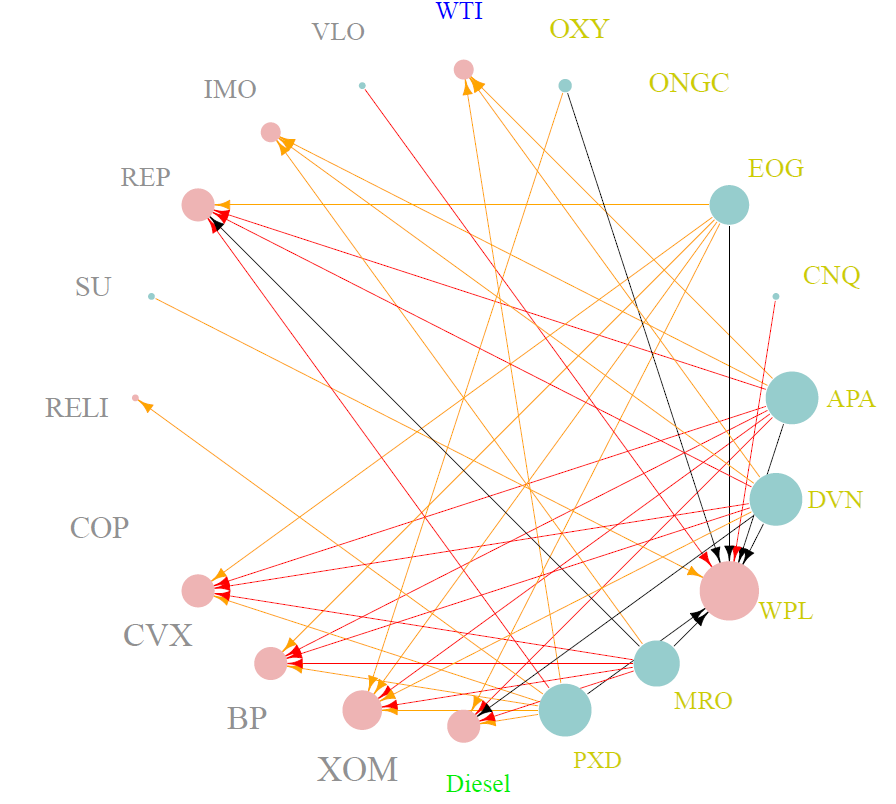
\includegraphics[width=\linewidth]{static_net2}
\caption{\textbf{A volatilitás átterjedésének iránya és erőssége a hálózatban}}

\end{subfigure}%
\begin{subfigure}{.5\linewidth}
\centering
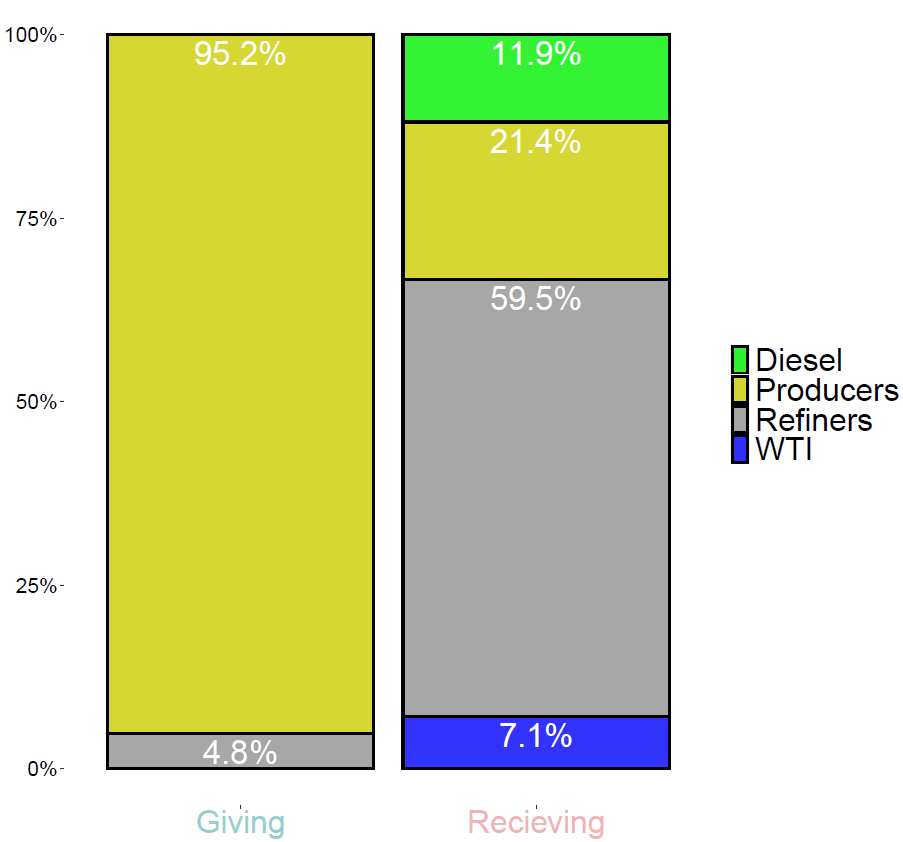
\includegraphics[width=\linewidth]{barchart}
\caption{\textbf{Az átterjedt volatilitás megoszlása}}
\end{subfigure}\\[1ex]
\end{figure}

%----------------------------------------------------------------------------------------------------------------------------------------------------

\subsubsection{Dinamikus eredmények}

A statikus elemzés önmagában is árulkodó lehet az iparág sajátosságairól, de a kapcsolatok időbeli dinamikáját nem képes bemutatni, így egy gördülő ablakos elemzést is elvégzek. A teljes hálózat összesített átterjedési indexét a 10. ábra prezentálja. A mellékletben megtalálható 13. ábra a szereplőkként felösszegzett nettó volatilitásátterjedést mutatja idősorosan.

%------------------------------------------------------------------------fig10----------------------------------------------------------------------------
\begin{figure}[H]
\caption{A teljes hálózatot jellemző átterjedési index időbeli alakulása}
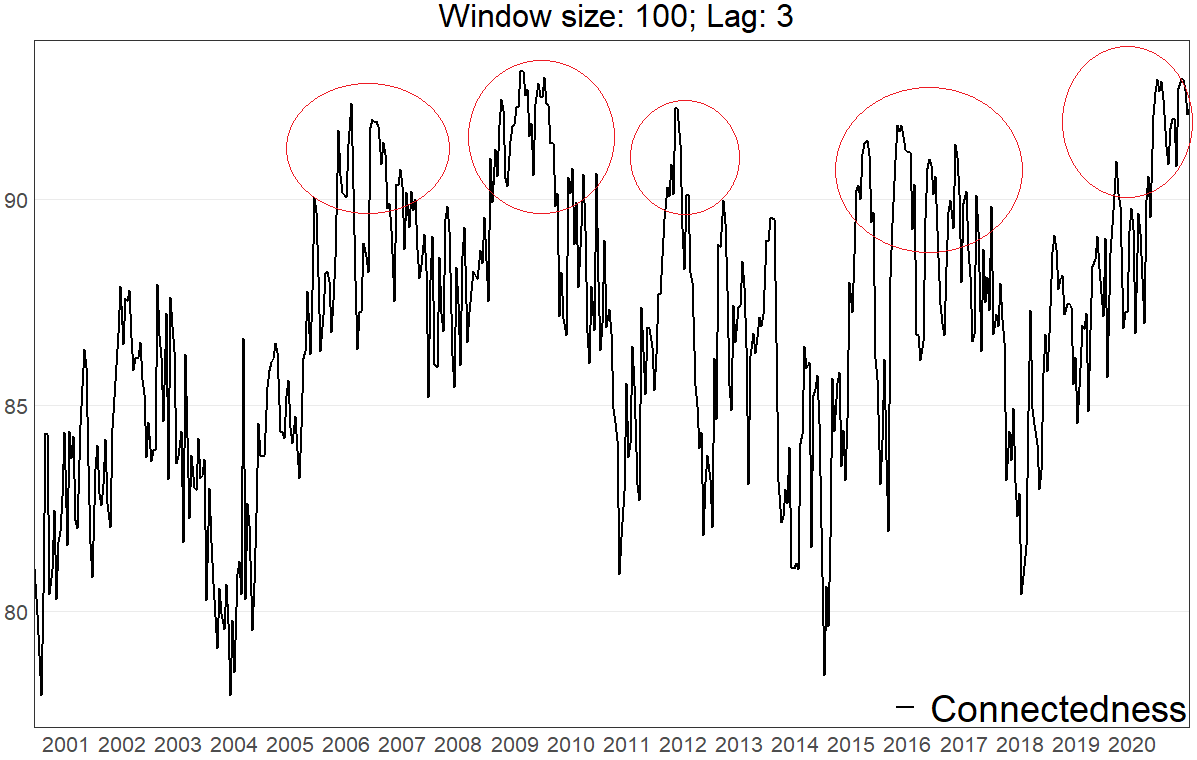
\includegraphics[width=11.5cm]{connectedness}
\centering
\end{figure}
%----------------------------------------------------------------------------------------------------------------------------------------------------

Az ablakméret hossza 100 megfigyelés és az ugrás hossza pedig 10 nap (két kereskedési hét). Ezek a hivatkozott források alapján megválasztott paraméterek, érdemes a modellt más számokkal is újrafuttatni, az eredmények megbízhatóságának belátása érdekében. Az ábrán az látható, hogy a teljes összekötöttségi index a vizsgált periódus alatt végig nagyon magas, a trajektória 71 és 92\% között ingadozik. Ez jóval meghaladja a \cite{diebold2012better} pénzügyi részvények ugyanezen vizsgálat következtében kapott eredményeit. (A szerzőpáros 56 és 89\% közötti eredményeket dokumentálnak, melyeket szintén magasnak ítelnek meg.) 

A vizsgált 21 év alatt, öt esetben lépte át az index a 90\%-os határt. Ezeket a következő világpiaci, gazdasági események okozhatták:

\begin{itemize}
\item 2006-2007: Izrael és Libanon közötti konfliktus, az iráni atomprogram bizonytalanságai és a Katrina hurrikán együttes hatásai.
\item 2008-2010: A subprime válság.
\item 2012: A Seaway olajcső áramlási irányának megfordítása.
\item 2016: Az OPEC országok egyezménye alapján napi 1.8 millió hordónyi nyersolajjal csökkentették a termelést az ár emelésének érdekében.
\item 2019-2020: A COVID-19 járvány közlekedési iparra gyakorolt hatása.
\end{itemize}

A rendszer mikro-szintjén is azonosíthatunk sokkokat, melyeknek hatására egy (vagy több) entitás volatilitás leadása megnövekszik egy időre. Három ilyen példát szemléltet a 11-es ábra. 2004-ben egy hatalmas gázmezőt fedeztek fel a Krishna Godavari medencében, Indiában. A hír hatására a két indiai vállalat részvényeinek árfolyama 70\%-kal emelkedett, majd fél év alatt, nagy esésekkel, visszacsökkent az eredeti szintjére (11. (a) ábra). 

2010-ben megtörtént az egyik legnagyobb olajiparhoz tartozó katasztróka, a Mexikói-öbölben lévő Deepwater Horizon fúrótorony felrobbant és 780 ezer m\textsuperscript{3} olaj árasztotta el a tengert. A létesítmény a BP tulajdonában volt, mely cég árfolyama, pár nap leforgása alatt 630 angol fontról 357-re esett vissza (és azóta sem tudta ezt a szintet elérni soha.)(11. (b) ábra).

Az oklahomai Cushing városban keresztezik egymást az amerikai kontinens legfontosabb olajvezetékei. 2012-ig az volt a jellemző, hogy az ide beérkező nyersolajat itt dolgozzák fel, azonban ebben az évben a Seaway cső irányát megfordították a kihasználatlanság miatt. Az évek alatt a Mexikói-öbölben korszerűbb és nagyobb kapacitású finomítók épültek ki, így költséghatékonyabb lett, az itt feldolgozott és innen tanker hajókon tovább szállított olaj. Az esemény hatására a WTI és a Brent közötti felár 19 dollárról 15-re csökkent. (11. (c) ábra)

%------------------------------------------------------------------------fig10----------------------------------------------------------------------------

\begin{figure}[H]
\centering
\caption{Olajipari sokkok, mikro szinten}
\begin{subfigure}{.5\linewidth}
\centering
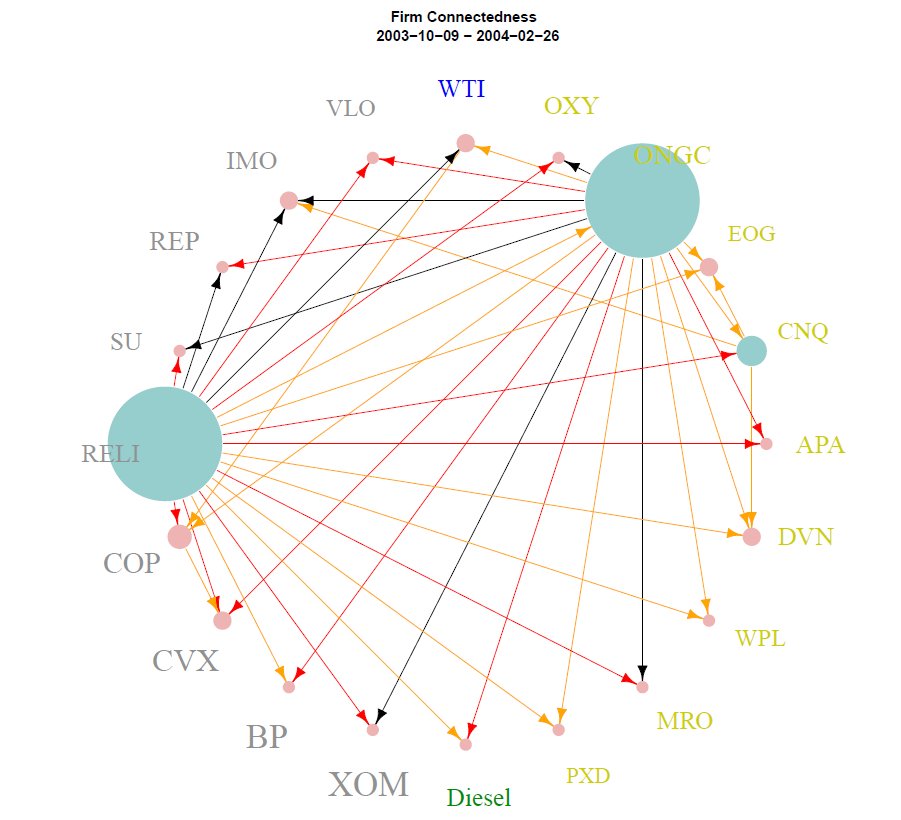
\includegraphics[width=\linewidth]{reli}
\caption{\textbf{Indiai gázmező}}

\end{subfigure}%
\begin{subfigure}{.5\linewidth}
\centering
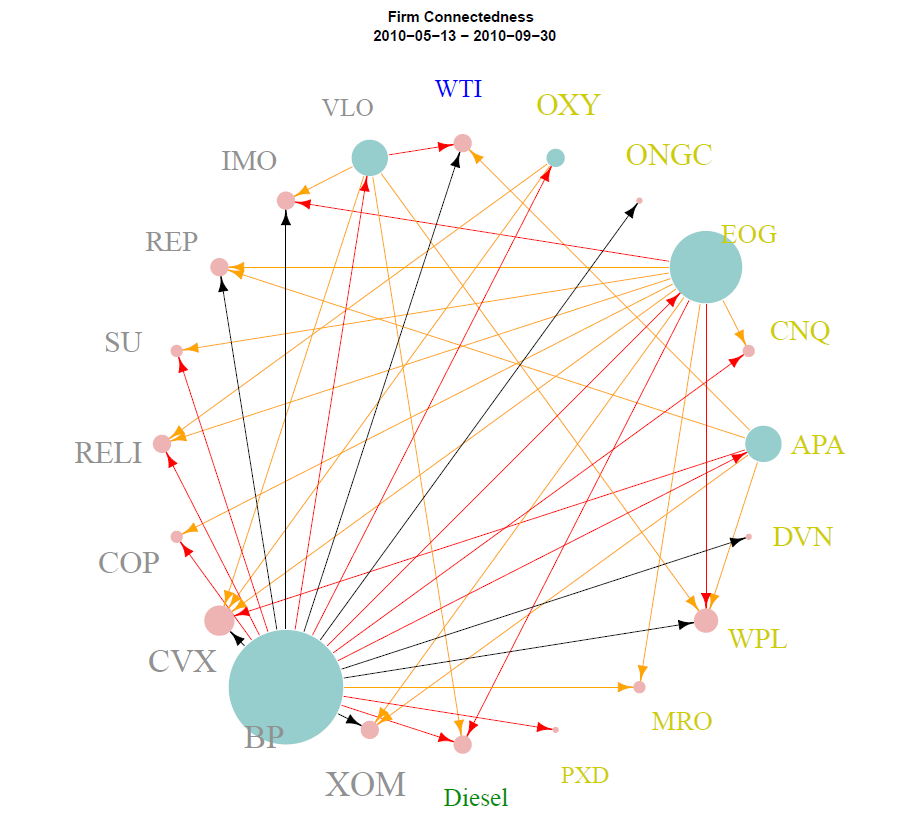
\includegraphics[width=\linewidth]{bp2}
\caption{\textbf{Deepwater Horizon fúrótorony}}
\end{subfigure}\\[1ex]
\begin{subfigure}{.5\linewidth}
\centering
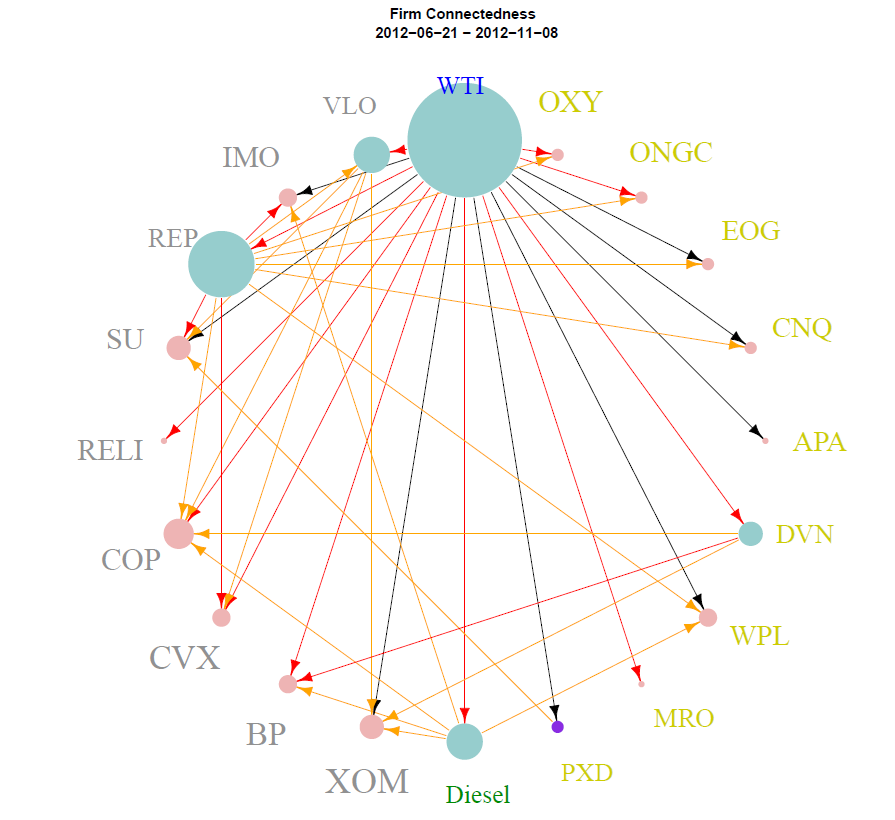
\includegraphics[width=\linewidth]{wti}
\caption{\textbf{Seeway olajcső}}
\end{subfigure}
\end{figure}

%----------------------------------------------------------------------------------------------------------------------------------------------------

A volatilitás leadásának és felvételének eloszlását a 12. ábra mutatja a teljes peródust tekintve. A bal oldali részábrán a sárga szín dominál, mely a kitermelőket reprezentája. Ez azt jelenti, hogy a volatilitás többségében a kitermelő vállaltoktól származik. Ez a hatás az elmúlt években erősödött, a 2000-es évek elején még nagyobb részt vállaltak a volatilitás terjesztéséből a finomítók. A származtatott termékek közül a WTI képes jelentős átadóvá válni, de csak rövid időre. Ezeket a periódusokat a kék ''tüskék'' ábrázolják.

Rövid, pár hetes periódusoktól eltekintve, a volatilitás több mint felét a teljes időszak alatt a finomítók vették fel. A WTI-nak a válságos periódusok alatt (2006-2007, 2008-2010, 2020) nagyobb rész jut, míg a a Diesel körülbelül 10\% körül ingadozik. Az ábra alapján a recessziós periódusokban a derivatívák átveszik az olajfinomítók volatilitáselnyelő szerepét.

%------------------------------------------------------------------------fig10----------------------------------------------------------------------------
\begin{figure}[H]
\centering
\caption{A volatilitás terjedése dinamikusan ábrázolva és szereplőkként csoportosítva}
\begin{subfigure}{.5\linewidth}
\centering
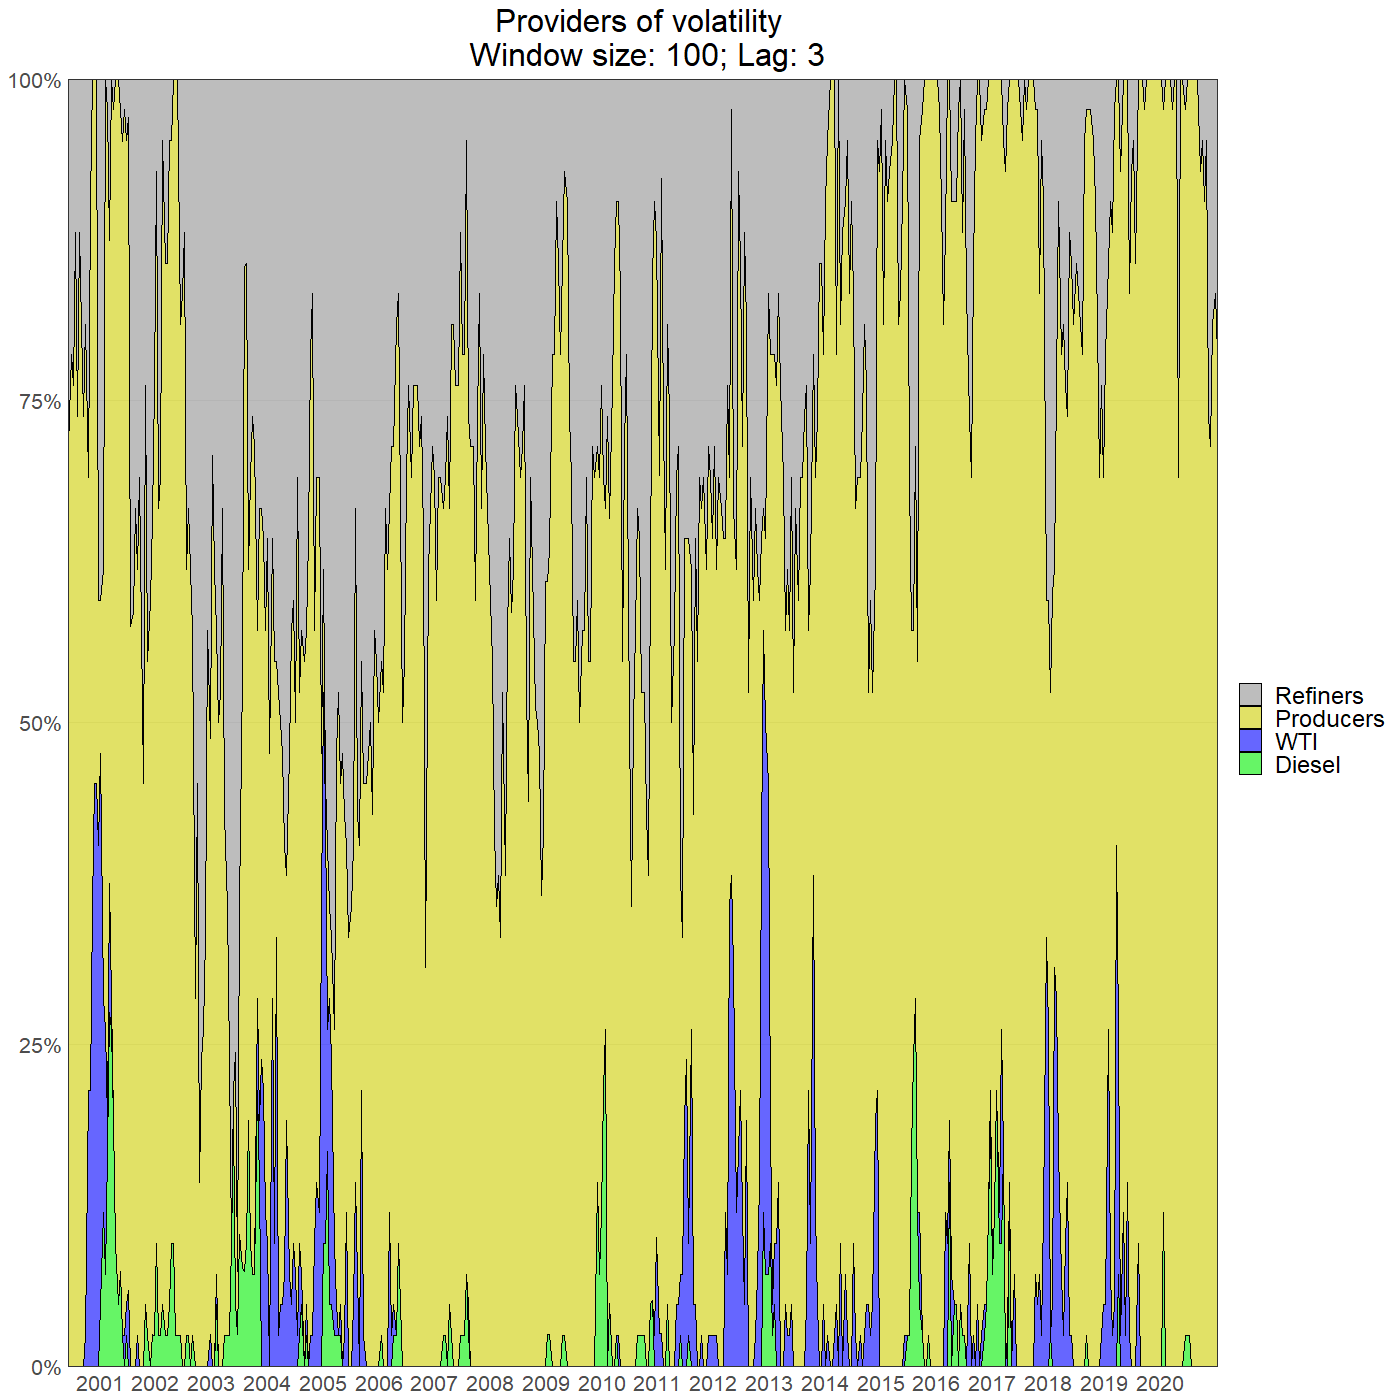
\includegraphics[width=\linewidth]{provv}
\caption{\textbf{Volatilitás átadók}}

\end{subfigure}%
\begin{subfigure}{.5\linewidth}
\centering
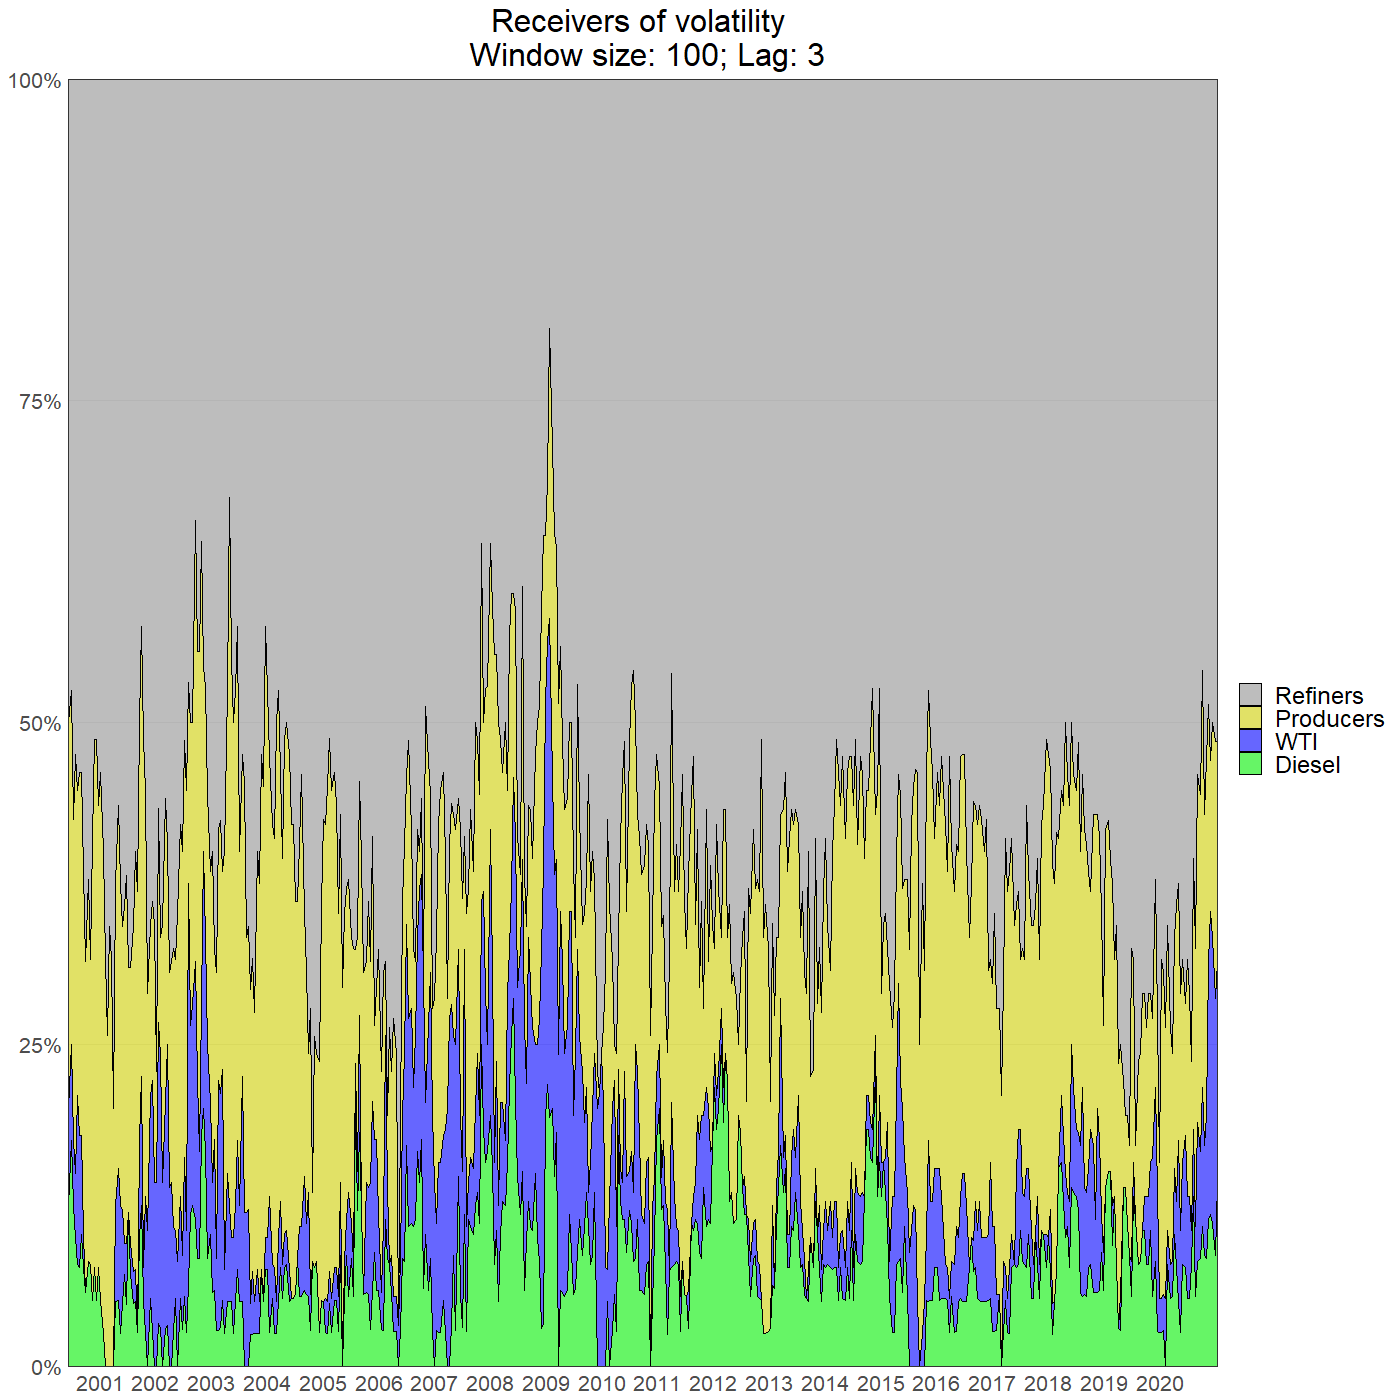
\includegraphics[width=\linewidth]{recc}
\caption{\textbf{Volatilitás felvevők}}
\end{subfigure}\\[1ex]
\end{figure}

%------------------------------------------------------------------------fig12----------------------------------------------------------------------------




\subsection{Konklúzió és további tervek}
Tanulmányom jelenlegi formájában képes azonosítani az olajpiacon történt sokkokat, továbbá azt mutatja be, hogy a volatilitás többségében a kitermelők felől áramlik a finomítók felé, mely hatás az elmúlt 21 évben csak erősödött. Azonban ezt az állítást még nem tartom kellően robosztusnak, szereném további vizsgálatokkal megerősíteni. Egyelőre egy alapvető módszer, a SIC kód alapján kategorizálom a cégeket, mely csak az elsődleges profil mutatója. A vizsgált vállalatok a világ legnagyobbjainak tekinthetők (az XOM valóban évekig a Föld legnagyobb cége volt, kapitalizációja alapján), így természetesen az olajpiac több szegmenségen is tevékenykedik. Besorolásom az éves jelentések alapján tovább finomítható, ott a bevétel megjelenik különböző iparágak szerinti bontásban is. A vizsgált periódus rövidítésével több hatalmas szereplő is bekerülhetne az elemzésbe, illetve megfontolandó a mostani univerzum egyes elemeinek lecserélése is. Láthattuk, hogy a WLP és a két indiai cég a többitől erősen eltérő viselkedést mutat, ezért torzítják az eredményeket. Egy tisztán amerikai tőzsdéken kereskedett részvényekből álló portfólión is szeretném elvégezni az analízist, valamint szeretnék kontrollváltozót is bevonni. \cite{kilian2009not} azonosítja a kereslet és kínálat okozta árváltozásokat az olajpiacon. Az ő tanulmányát is szeretném integrálni a kutatásomba. 

A volatilitás számítása esetén kiemeltem, hogy az egyszerűség miatt döntöttem a Parkinson-féle volatilitási mérték alkalmazása mellett. Mivel rengeteg forrás támaszkodik a GARCH modellcsalád valamelyikére, robosztusságvizsgálat keretei között az ily módon kalkulált volatilitást is górcső alá fogom vonni. A jelenlegi időablak önkényes módon 100 nap, mely változtatásával szintén az eredményeim hitelességét kívánom megerősíteni.



\newpage

\section{Összefoglalás és további elképzelések}

Kutatási tanulmányomban először röviden bemutattam a pénzügyi hálózatokban definiálható kapcsolatok irodalmát. Természetesen az áttekintés távolról sem teljes körű, csak a legrelevánsabb cikkeket hivatkoztam le, ezen munkám formai megkötései miatt. A diszertációm megírásakor szeretném sokkal részletesebben bemutatni az Acemoglu és Elliott értekezéseihez hasonló elméleti megközelítéséket is. Továbbá úgy érzem, a részvények összekötöttségével foglalkozó irodalmi tudásom még hiányos, ebben a témakörben még olvasnom kell.

A második fejezetben egy olyan tanulmányt prezentálok melyben a Toda-Yamamoto okságon alapuló modell alapján kapcsolatokat határozok meg országok hozamgörbe faktorai között. Ered-ményeim szerint, a rendszert az Egyesült Államok dominálja. Idősorosan vizsgálódva azt kaptam, hogy a válságos periódusokban a hálózat sűrűbbé válik (megnő a kapcsolatok száma), mely a hasonló témájú cikkek konklúziójával is összecseng. Milánnal arra gondoltunk, hogy végleges cikkünket a Journal of International Financial Markets, Institutions and Money folyóirathoz szerenénk beküldeni 2021 második felében.

A harmadik fejezetben az olajipari részvények (és árupiaci termékek) piacán realizált volatilitás átterjedését tanulmányoztam a Diebold-Yilmaz módszerrel. Statikus eredményeim alapján azt mondhatom, hogy a volatilitást az olajkitermelők gerjesztik, míg az olajfinomítók felveszik. Ahogy az előző esetben is, válságos periódusban a teljes hálózatot jellemző átterjedési index megnövekedett, valamint sikerrel tudtam azonosítani olyan történéseket, melyek rövid időre sokkolták a rendszert. Dinamikus megközelítésem alátámasztja a statikus modell alapján állítottakat, historikusan nézve is, a kitermelők felelősek a volatilitás leadásáért, a finomítók a felvételért. A nyersolaj időszakosan volatilitás leadó szerepet vesz fel. Amennyiben a fent bemutatott tervek releváns eredményeket hoznak, úgy Martinnal az Energy Economics-ot fogjuk felkeresni a cikkel.

A fent említetteken kívül Martinnal egy további magyar cikket is tervezünk megjelentetni, elképzeléseink alapján 2022-ben. Itt az alacsony és magas ESG besorolású részvényportfóliók közötti hozamátterjedést szeretnénk megvizsgálni a \cite{adrian2008federal} és \cite{hardle2016tenet} által definiált CoVar-TENET Value at Risk (V@R) alapú átterjedési mérték alapján. Jelenleg ez csak ötlet szinten fogalmazódott meg, a tényleges kutatást idén ősszel kezdjük. 

A végső disszertációmhoz, mindezeken túl, még meg kell vizsgálnom a CDS-ek és a devizaárfolyamok közötti kapcsolatokat. Utóbbi hozamainak és volatilitásának átterjedése esetén a második fejezetben felvázolt Diebold-Yilmaz módszer terjedt el, így én is ezt fogom alkalmazni (\cite{greenwood2016risk}). A CDS-ek esetén \cite{markose2012too} munkáját veszem majd alapul, akik egy Erdős-Rényi gráf segítségével határoztak meg kapcsolatokat.

Miután minden alrendszerben megkaptam a dinamikus összekötöttségi mértéket, ezeket aggregálni fogom egy idősor klasszifikációs eljárással. Az erre legalkalmasabb megoldást még nem találtam meg, a \cite{fawaz2020inceptiontime} által javasolt mélytanuló neurális lehet célravezető.

A piacokat érintő sokkok különböző eszközökön keresztül, különböző módon terjednek tovább, ezért a hatékonyabb reakció érdekében szükséges dinamikájuk megértése mind a szabályozók, mind a többi piaci résztvevő számára. Az összekötöttségi hálózati struktúrák ismerete hasznos a lehetséges károk csökkentése és a megfelelő jövőbeni döntések meghozatala szempontjából. A különféle eszközök összekapcsoltságának elemzése döntő szerepet játszik a rendszerkockázat értékelésben és kezelésében. Disszertációmmal ezt az irodalmat kívánom bővíteni és egy új megkö-zelítési módszer segítségével definiálni a ''Túl Beágyazott, hogy Elbukjon'' (Too Interconnected to Fail) típusú szereplőket.

\newpage


\bibliographystyle{te}


\bibliography{research}





\begin{appendices}



\begin{table}[H]
\caption{A választott országok hozamgörbepoinjainak leíró statisztikája}% title of Table
\fontsize{9}{9}\selectfont
\centering % used for centering table
\begin{tabular}{l c c c c c c}% centered columns (4 columns)
\hline\hline   \\ [-1.5ex]               %inserts double horizontal lines
%Case & Method\#1 & Method\#2 & Method\#3 & test \\  [0.5ex]
Lejárat & Átlag & Szórás & Minimum & Maximum & \textrho(1)  & \textrho(10) \\ [0.5ex] % inserts table %heading

\hline       \\ [-1.5ex]           % inserts single horizontal line
\textit{Németország} 	&		&		&		&		&		&	\\
1 év	&	0.0256	&	1.6275	&	-0.9690	&	4.6900	&	1.0000	&	0.9960	\\
5 év	&	0.0257	&	1.6324	&	-0.9410	&	4.7670	&	0.9990	&	0.9930	\\
10 év	&	0.0243	&	1.5451	&	-0.7220	&	4.6860	&	0.9930	&	0.9640	\\
\medskip													
30 év	&	0.0228	&	1.4482	&	-0.2440	&	5.1950	&	0.9990	&	0.9880	\\
\textit{Olaszotszág}	&		&		&		&		&		&		\\
1 év	&	0.0241	&	1.5327	&	-0.4840	&	8.3940	&	0.9980	&	0.9860	\\
5 év	&	0.0239	&	1.5199	&	0.2370	&	7.8950	&	0.9980	&	0.9850	\\
10 év	&	0.0218	&	1.3876	&	0.8750	&	7.4920	&	0.9980	&	0.9860	\\
\medskip													
30 év	&	0.0188	&	1.1971	&	2.0430	&	7.5840	&	0.9980	&	0.9850	\\
\textit{Franciaország}	&		&		&		&		&		&		\\
1 év	&	0.0250	&	1.5891	&	-0.8010	&	4.6570	&	1.0000	&	0.9960	\\
5 év	&	0.0247	&	1.5730	&	-0.7730	&	4.9100	&	0.9990	&	0.9930	\\
10 év	&	0.0231	&	1.4670	&	-0.4150	&	4.8510	&	0.9990	&	0.9910	\\
\medskip													
30 év	&	0.0194	&	1.2351	&	0.4190	&	5.1160	&	0.9990	&	0.9860	\\
\textit{USA}	&		&		&		&		&		&		\\
1 év	&	0.0254	&	1.6128	&	0.0540	&	5.3230	&	1.0000	&	0.9980	\\
5 év	&	0.0194	&	1.2315	&	0.5590	&	5.3010	&	0.9990	&	0.9890	\\
10 év	&	0.0163	&	1.0394	&	1.3890	&	5.3880	&	0.9980	&	0.9830	\\
\medskip
30 év	&	0.0151	&	0.9618	&	1.9920	&	5.8390	&	0.9970	&	0.9760	\\
\textit{Kanada}	&		&		&		&		&		&		\\
1 év	&	0.0193	&	1.2301	&	0.3000	&	4.8090	&	1.0000	&	0.9950	\\
5 év	&	0.0180	&	1.1463	&	0.4840	&	4.8010	&	0.9990	&	0.9890	\\
10 év	&	0.0173	&	1.0976	&	0.9830	&	5.0760	&	0.9990	&	0.9870	\\
\medskip													
30 év	&	0.0159	&	1.0118	&	1.3060	&	5.6120	&	0.9980	&	0.9850	\\
\textit{Mexikó}	&		&		&		&		&		&		\\
1 év	&	0.0318	&	2.0250	&	1.5120	&	10.5700	&	0.9790	&	0.9880	\\
5 év	&	0.0238	&	1.5108	&	3.7860	&	10.8970	&	0.9860	&	0.9810	\\
10 év	&	0.0213	&	1.3524	&	4.6190	&	12.4130	&	0.9920	&	0.9700	\\
\medskip
30 év	&	0.0195	&	1.2384	&	5.8730	&	12.7260	&	0.9930	&	0.9470	\\
\textit{Japán}	&		&		&		&		&		&		\\
1 év	&	0.0043	&	0.2715	&	-0.3710	&	0.8500	&	0.9990	&	0.9920	\\
5 év	&	0.0076	&	0.4852	&	-0.3960	&	1.6310	&	0.9990	&	0.9900	\\
10 év	&	0.0103	&	0.6563	&	-0.2850	&	2.0500	&	0.9990	&	0.9900	\\
\medskip													
30 év	&	0.0120	&	0.7606	&	0.0530	&	3.2950	&	0.9980	&	0.9850	\\
\textit{Kína}	&		&		&		&		&		&		\\
1 év	&	0.0115	&	0.7296	&	0.9570	&	4.3820	&	0.9920	&	0.9660	\\
5 év	&	0.0093	&	0.5939	&	1.7820	&	4.8740	&	0.9970	&	0.9730	\\
10 év	&	0.0090	&	0.5702	&	2.4810	&	5.5030	&	0.9930	&	0.9640	\\
\medskip													
30 év	&	0.0097	&	0.6149	&	2.4700	&	6.0090	&		&		\\
\textit{Ausztrália}	&		&		&		&		&		&		\\
1 év	&	0.0279	&	1.7749	&	0.6750	&	7.3760	&	0.9990	&	0.9920	\\
5 év	&	0.0264	&	1.6769	&	0.6390	&	6.9600	&	0.9990	&	0.9900	\\
10 év	&	0.0235	&	1.4971	&	0.8850	&	6.8730	&	0.9990	&	0.9880	\\
\medskip													
30 év	&	0.0190	&	1.2069	&	1.5580	&	6.8880	&	0.9980	&	0.9830	\\
\textit{Norvégia}	&		&		&		&		&		&		\\
1 év	&	0.0222	&	1.4100	&	0.1990	&	6.2430	&	0.9990	&	0.9940	\\
5 év	&	0.0200	&	1.2734	&	0.5450	&	5.3350	&	0.9990	&	0.9910	\\
10 év	&	0.0188	&	1.1935	&	0.8880	&	5.2760	&	0.9990	&	0.9890	\\
\medskip													
30 év	&	0.0175	&	1.1127	&	0.8820	&	5.2730	&	0.9990	&	0.9870	\\
\textit{Egyesült Királyság}	&		&		&		&		&		&		\\
1 év	&	0.0308	&	1.9558	&	0.0240	&	5.8830	&	0.9990	&	0.9950	\\
5 év	&	0.0259	&	1.6444	&	0.1610	&	5.8210	&	0.9990	&	0.9910	\\
10 év	&	0.0223	&	1.4181	&	0.4000	&	5.5430	&	0.9990	&	0.9890	\\
\medskip													
30 év	&	0.0175	&	1.1099	&	0.9390	&	5.0700	&	0.9990	&	0.9870	\\
\textit{Svájc}	&		&		&		&		&		&		\\
1 év	&	0.0195	&	1.2405	&	-1.1650	&	3.3750	&	1.0000	&	0.9960	\\
5 év	&	0.0187	&	1.1921	&	-1.1960	&	3.2000	&	0.9990	&	0.9930	\\
10 év	&	0.0188	&	1.1976	&	-1.1380	&	3.4550	&	0.9990	&	0.9910	\\
30 év	&	0.0173	&	1.1006	&	-0.6440	&	3.7330	&	0.9980	&	0.9860	\\

\hline%inserts single line
\end{tabular}
\label{table:nonlin}% is used to refer this table in the text
\end{table}
%----------------------------------------------------------------------------------------------------------------------------------------------------


\begin{figure}[ht]
\caption{Szereplőkként felösszegzett nettó volatilitásátterjedés}
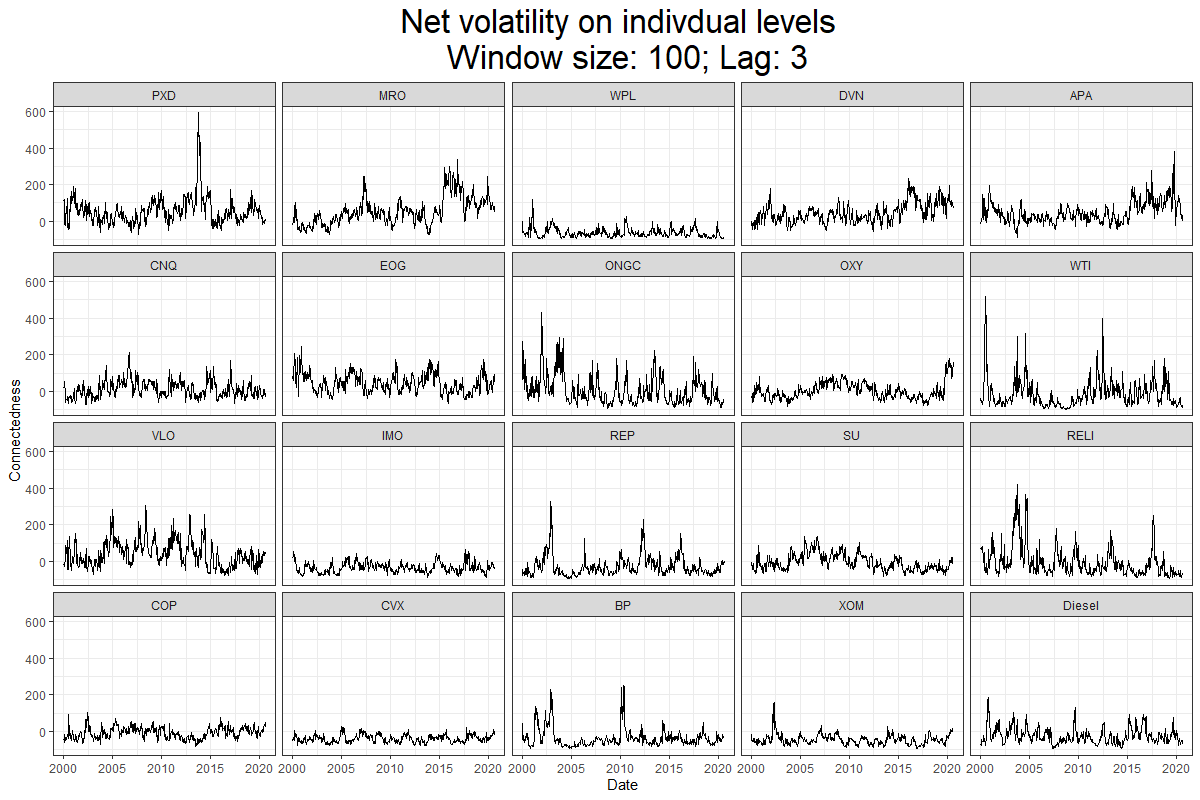
\includegraphics[width=17cm]{vol_net}
\centering
\end{figure}

%----------------------------------------------------------------------------------------------------------------------------------------------------

%----------------------------------------------------------------------------------------------------------------------------------------------------

\end{appendices}


\newpage 






\end{document}

